% Options for packages loaded elsewhere
\PassOptionsToPackage{unicode}{hyperref}
\PassOptionsToPackage{hyphens}{url}
\PassOptionsToPackage{dvipsnames,svgnames,x11names}{xcolor}
%
\documentclass[
  letterpaper,
  DIV=11,
  numbers=noendperiod]{scrreport}

\usepackage{amsmath,amssymb}
\usepackage{iftex}
\ifPDFTeX
  \usepackage[T1]{fontenc}
  \usepackage[utf8]{inputenc}
  \usepackage{textcomp} % provide euro and other symbols
\else % if luatex or xetex
  \usepackage{unicode-math}
  \defaultfontfeatures{Scale=MatchLowercase}
  \defaultfontfeatures[\rmfamily]{Ligatures=TeX,Scale=1}
\fi
\usepackage{lmodern}
\ifPDFTeX\else  
    % xetex/luatex font selection
\fi
% Use upquote if available, for straight quotes in verbatim environments
\IfFileExists{upquote.sty}{\usepackage{upquote}}{}
\IfFileExists{microtype.sty}{% use microtype if available
  \usepackage[]{microtype}
  \UseMicrotypeSet[protrusion]{basicmath} % disable protrusion for tt fonts
}{}
\makeatletter
\@ifundefined{KOMAClassName}{% if non-KOMA class
  \IfFileExists{parskip.sty}{%
    \usepackage{parskip}
  }{% else
    \setlength{\parindent}{0pt}
    \setlength{\parskip}{6pt plus 2pt minus 1pt}}
}{% if KOMA class
  \KOMAoptions{parskip=half}}
\makeatother
\usepackage{xcolor}
\setlength{\emergencystretch}{3em} % prevent overfull lines
\setcounter{secnumdepth}{5}
% Make \paragraph and \subparagraph free-standing
\ifx\paragraph\undefined\else
  \let\oldparagraph\paragraph
  \renewcommand{\paragraph}[1]{\oldparagraph{#1}\mbox{}}
\fi
\ifx\subparagraph\undefined\else
  \let\oldsubparagraph\subparagraph
  \renewcommand{\subparagraph}[1]{\oldsubparagraph{#1}\mbox{}}
\fi


\providecommand{\tightlist}{%
  \setlength{\itemsep}{0pt}\setlength{\parskip}{0pt}}\usepackage{longtable,booktabs,array}
\usepackage{calc} % for calculating minipage widths
% Correct order of tables after \paragraph or \subparagraph
\usepackage{etoolbox}
\makeatletter
\patchcmd\longtable{\par}{\if@noskipsec\mbox{}\fi\par}{}{}
\makeatother
% Allow footnotes in longtable head/foot
\IfFileExists{footnotehyper.sty}{\usepackage{footnotehyper}}{\usepackage{footnote}}
\makesavenoteenv{longtable}
\usepackage{graphicx}
\makeatletter
\def\maxwidth{\ifdim\Gin@nat@width>\linewidth\linewidth\else\Gin@nat@width\fi}
\def\maxheight{\ifdim\Gin@nat@height>\textheight\textheight\else\Gin@nat@height\fi}
\makeatother
% Scale images if necessary, so that they will not overflow the page
% margins by default, and it is still possible to overwrite the defaults
% using explicit options in \includegraphics[width, height, ...]{}
\setkeys{Gin}{width=\maxwidth,height=\maxheight,keepaspectratio}
% Set default figure placement to htbp
\makeatletter
\def\fps@figure{htbp}
\makeatother
\newlength{\cslhangindent}
\setlength{\cslhangindent}{1.5em}
\newlength{\csllabelwidth}
\setlength{\csllabelwidth}{3em}
\newlength{\cslentryspacingunit} % times entry-spacing
\setlength{\cslentryspacingunit}{\parskip}
\newenvironment{CSLReferences}[2] % #1 hanging-ident, #2 entry spacing
 {% don't indent paragraphs
  \setlength{\parindent}{0pt}
  % turn on hanging indent if param 1 is 1
  \ifodd #1
  \let\oldpar\par
  \def\par{\hangindent=\cslhangindent\oldpar}
  \fi
  % set entry spacing
  \setlength{\parskip}{#2\cslentryspacingunit}
 }%
 {}
\usepackage{calc}
\newcommand{\CSLBlock}[1]{#1\hfill\break}
\newcommand{\CSLLeftMargin}[1]{\parbox[t]{\csllabelwidth}{#1}}
\newcommand{\CSLRightInline}[1]{\parbox[t]{\linewidth - \csllabelwidth}{#1}\break}
\newcommand{\CSLIndent}[1]{\hspace{\cslhangindent}#1}

\KOMAoption{captions}{tableheading}
\makeatletter
\makeatother
\makeatletter
\@ifpackageloaded{bookmark}{}{\usepackage{bookmark}}
\makeatother
\makeatletter
\@ifpackageloaded{caption}{}{\usepackage{caption}}
\AtBeginDocument{%
\ifdefined\contentsname
  \renewcommand*\contentsname{Table of contents}
\else
  \newcommand\contentsname{Table of contents}
\fi
\ifdefined\listfigurename
  \renewcommand*\listfigurename{List of Figures}
\else
  \newcommand\listfigurename{List of Figures}
\fi
\ifdefined\listtablename
  \renewcommand*\listtablename{List of Tables}
\else
  \newcommand\listtablename{List of Tables}
\fi
\ifdefined\figurename
  \renewcommand*\figurename{Figure}
\else
  \newcommand\figurename{Figure}
\fi
\ifdefined\tablename
  \renewcommand*\tablename{Table}
\else
  \newcommand\tablename{Table}
\fi
}
\@ifpackageloaded{float}{}{\usepackage{float}}
\floatstyle{ruled}
\@ifundefined{c@chapter}{\newfloat{codelisting}{h}{lop}}{\newfloat{codelisting}{h}{lop}[chapter]}
\floatname{codelisting}{Listing}
\newcommand*\listoflistings{\listof{codelisting}{List of Listings}}
\usepackage{amsthm}
\theoremstyle{definition}
\newtheorem{definition}{Definition}[chapter]
\theoremstyle{remark}
\AtBeginDocument{\renewcommand*{\proofname}{Proof}}
\newtheorem*{remark}{Remark}
\newtheorem*{solution}{Solution}
\makeatother
\makeatletter
\@ifpackageloaded{caption}{}{\usepackage{caption}}
\@ifpackageloaded{subcaption}{}{\usepackage{subcaption}}
\makeatother
\makeatletter
\@ifpackageloaded{tcolorbox}{}{\usepackage[skins,breakable]{tcolorbox}}
\makeatother
\makeatletter
\@ifundefined{shadecolor}{\definecolor{shadecolor}{rgb}{.97, .97, .97}}
\makeatother
\makeatletter
\makeatother
\makeatletter
\makeatother
\ifLuaTeX
  \usepackage{selnolig}  % disable illegal ligatures
\fi
\IfFileExists{bookmark.sty}{\usepackage{bookmark}}{\usepackage{hyperref}}
\IfFileExists{xurl.sty}{\usepackage{xurl}}{} % add URL line breaks if available
\urlstyle{same} % disable monospaced font for URLs
\hypersetup{
  pdftitle={Economics of Health Care},
  pdfauthor={Ian McCarthy},
  colorlinks=true,
  linkcolor={blue},
  filecolor={Maroon},
  citecolor={Blue},
  urlcolor={Blue},
  pdfcreator={LaTeX via pandoc}}

\title{Economics of Health Care}
\author{Ian McCarthy}
\date{2023-06-21}

\begin{document}
\maketitle
\ifdefined\Shaded\renewenvironment{Shaded}{\begin{tcolorbox}[sharp corners, enhanced, frame hidden, interior hidden, boxrule=0pt, breakable, borderline west={3pt}{0pt}{shadecolor}]}{\end{tcolorbox}}\fi

\renewcommand*\contentsname{Table of contents}
{
\hypersetup{linkcolor=}
\setcounter{tocdepth}{2}
\tableofcontents
}
\bookmarksetup{startatroot}

\hypertarget{welcome}{%
\chapter*{Welcome}\label{welcome}}
\addcontentsline{toc}{chapter}{Welcome}

\markboth{Welcome}{Welcome}

Health care is a vital component of our society, and it is essential to
understand the economic principles that underlie this complex system.
Health care economics is the study of how resources are allocated to
produce, distribute, and consume health care goods and services. It
encompasses a wide range of topics, including the behavior of health
care providers, the role of insurance and government policy, and the
impact of health care on the economy as a whole.

This book is intended to offer an introduction to the study of health
care economics. It covers key topics such as health insurance and health
care financing, physician behaviors, physician and hospital pricing, and
prescription drug markets. Within each topic, I present specific
theoretical models and discuss current health policy in the context of
those models. The material is intended for advanced undergraduate or
masters students with at least some exposure to intermediate-level
microeconomics.

Unfortunately, I can't cover everything in one introductory book -- nor
am I equipped to do so. One area that I've intentionally excluded from
this book is that of comparative health systems or any sort of
international view of health care. I'll use some basic international
comparisons in the introduction, but otherwise this is a very
U.S.-centric health economics book. Those interested in international
comparisons can find some great information from the
\href{https://www.healthsystemtracker.org/}{Peterson-KFF Health System
Tracker} and the
\href{https://www.commonwealthfund.org/international-health-policy-center/system-profiles}{Commonwealth
Fund}, among many other excellent resources. I've also excluded any
discussion of health care labor markets, such as nurse wages, physician
location and specialty selection, etc.

From this book, readers should be able to:

\begin{enumerate}
\def\labelenumi{\arabic{enumi}.}
\tightlist
\item
  Explain the structure of the U.S. health care system, its main
  components, and its history
\item
  Model adverse selection in health insurance, examine its effects on
  health insurance markets, and support your arguments with existing
  data
\item
  Explain the physician agency problem, use a model of physician agency
  to examine financial incentives in health care, and summarize
  empirical evidence on the presence of physician agency
\item
  Describe hospital pricing, negotiation with insurers, and explain
  (qualitatively and quantitatively) the differences between charges and
  prices
\item
  Analyze hospital data in a real-life setting and predict effects of
  real-life policies
\end{enumerate}

\hypertarget{health-improvements}{%
\section*{Health Improvements}\label{health-improvements}}
\addcontentsline{toc}{section}{Health Improvements}

\markright{Health Improvements}

Figure~\ref{fig-life-exp} presents the median life expectancy across the
world from around 1950 to 2010. As made clear from
Figure~\ref{fig-life-exp}, the world has witnessed significant progress
in improving life expectancy over the past several decades. This
progress can be attributed to several factors, including poverty
reduction, technological advancements, and increased access to critical
needs, including basic healthcare. As a result, people are living longer
and generally healthier lives, with fewer deaths from infectious
diseases and a higher quality of life in general.

\begin{figure}

{\centering 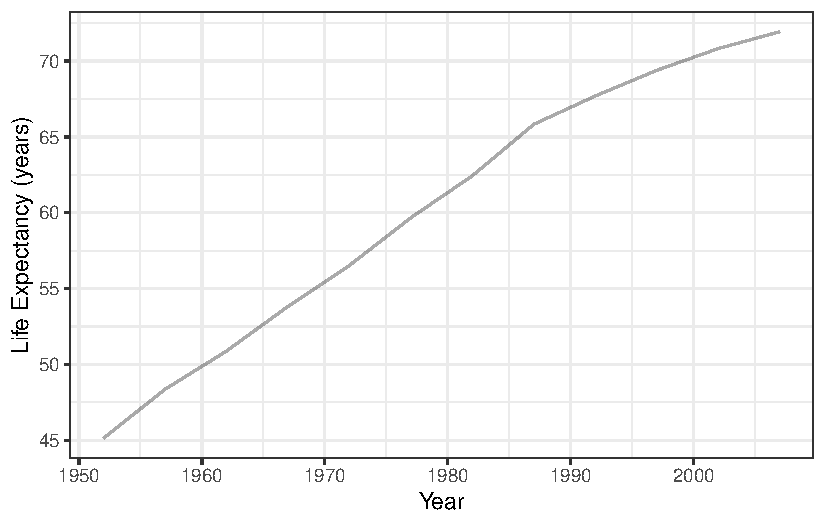
\includegraphics{index_files/figure-pdf/fig-life-exp-1.pdf}

}

\caption{\label{fig-life-exp}Median life expectancy across the world}

\end{figure}

\hypertarget{health-and-wealth}{%
\section*{Health and Wealth}\label{health-and-wealth}}
\addcontentsline{toc}{section}{Health and Wealth}

\markright{Health and Wealth}

Not surprisingly, gains in health are correlated with economic growth
and development, as illustrated in Figure~\ref{fig-life-exp-gdp}.

\begin{figure}

{\centering 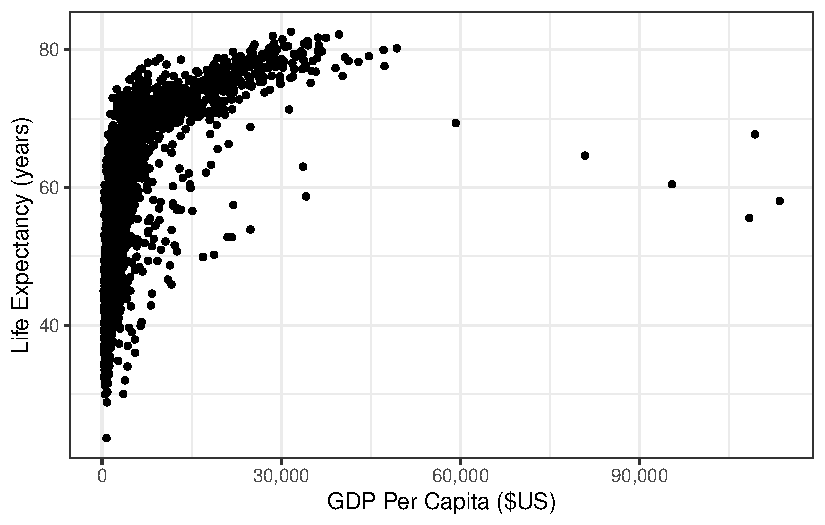
\includegraphics{index_files/figure-pdf/fig-life-exp-gdp-1.pdf}

}

\caption{\label{fig-life-exp-gdp}Life expectancy and GDP}

\end{figure}

This relationship between wealth and health is even more evident when we
look over time by country, as demonstrated in
\textbf{?@fig-anim-lifegdp}. This makes sense if we think of ways to
improve very low life expectancy (e.g., life expectancy cut due to lack
of basic necessities like food, shelter, clean water, basic medicine,
etc.).

\begin{figure}

{\centering 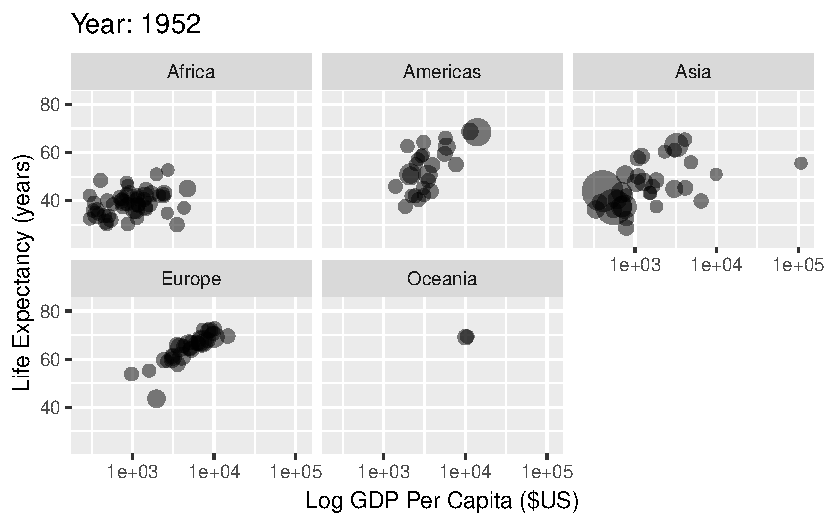
\includegraphics{index_files/figure-pdf/fig-anim-lifegdp-1.pdf}

}

\caption{\label{fig-anim-lifegdp-1}Life expectancy and GDP by country}

\end{figure}

\begin{figure}

{\centering 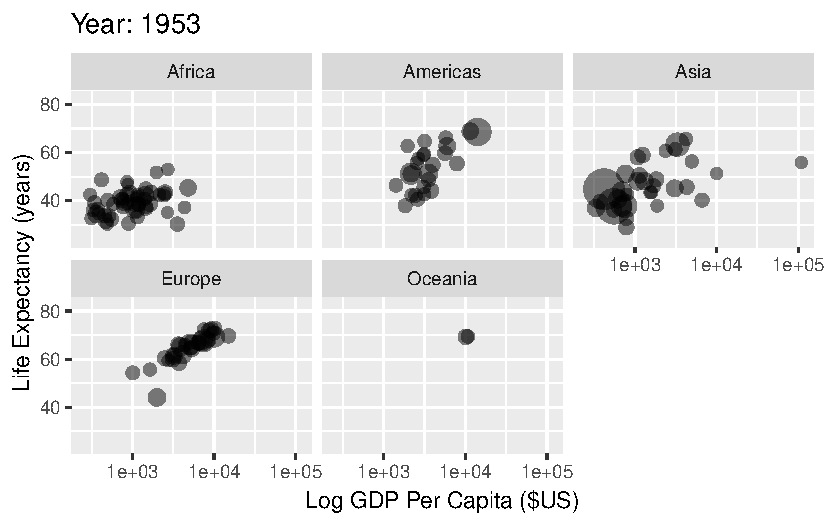
\includegraphics{index_files/figure-pdf/fig-anim-lifegdp-2.pdf}

}

\caption{\label{fig-anim-lifegdp-2}Life expectancy and GDP by country}

\end{figure}

\begin{figure}

{\centering 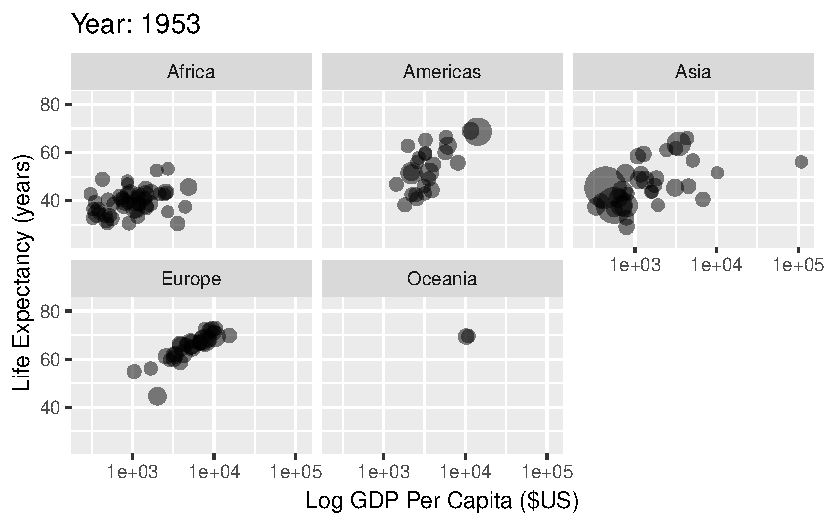
\includegraphics{index_files/figure-pdf/fig-anim-lifegdp-3.pdf}

}

\caption{\label{fig-anim-lifegdp-3}Life expectancy and GDP by country}

\end{figure}

\begin{figure}

{\centering 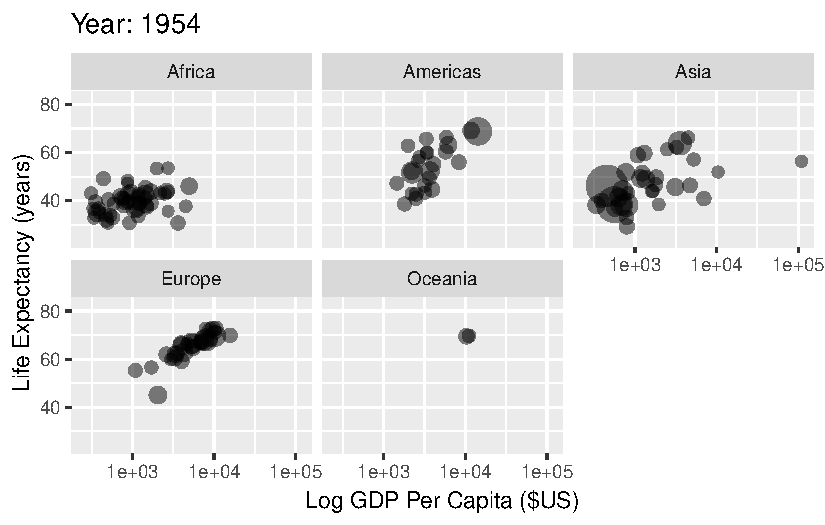
\includegraphics{index_files/figure-pdf/fig-anim-lifegdp-4.pdf}

}

\caption{\label{fig-anim-lifegdp-4}Life expectancy and GDP by country}

\end{figure}

\begin{figure}

{\centering 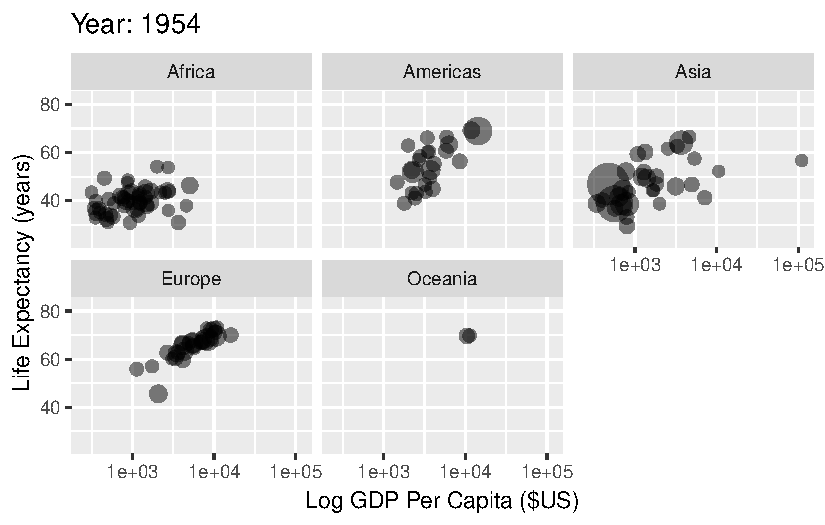
\includegraphics{index_files/figure-pdf/fig-anim-lifegdp-5.pdf}

}

\caption{\label{fig-anim-lifegdp-5}Life expectancy and GDP by country}

\end{figure}

\begin{figure}

{\centering 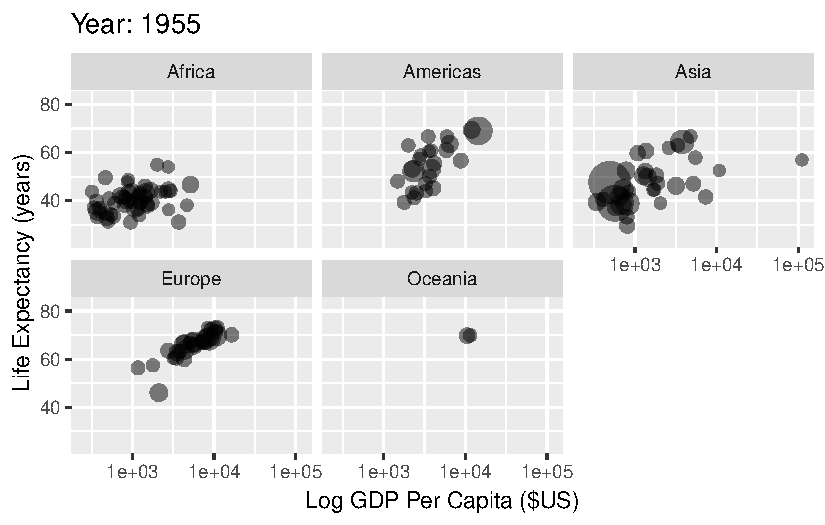
\includegraphics{index_files/figure-pdf/fig-anim-lifegdp-6.pdf}

}

\caption{\label{fig-anim-lifegdp-6}Life expectancy and GDP by country}

\end{figure}

\begin{figure}

{\centering 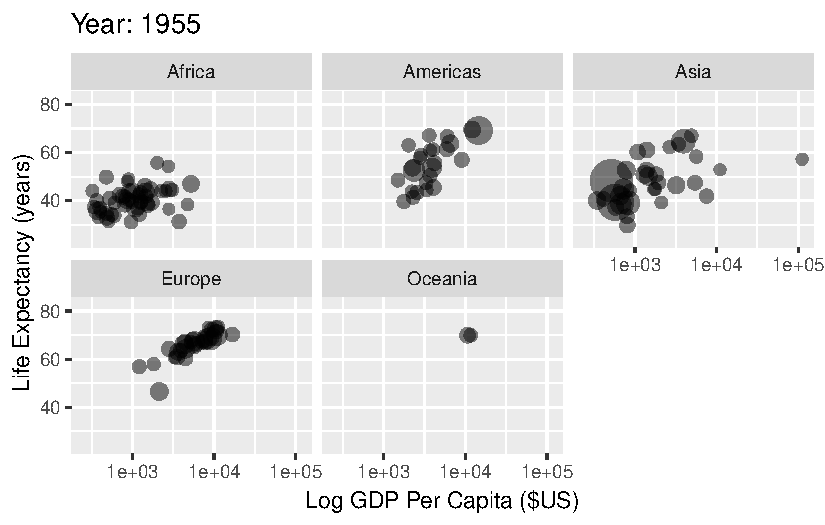
\includegraphics{index_files/figure-pdf/fig-anim-lifegdp-7.pdf}

}

\caption{\label{fig-anim-lifegdp-7}Life expectancy and GDP by country}

\end{figure}

\begin{figure}

{\centering 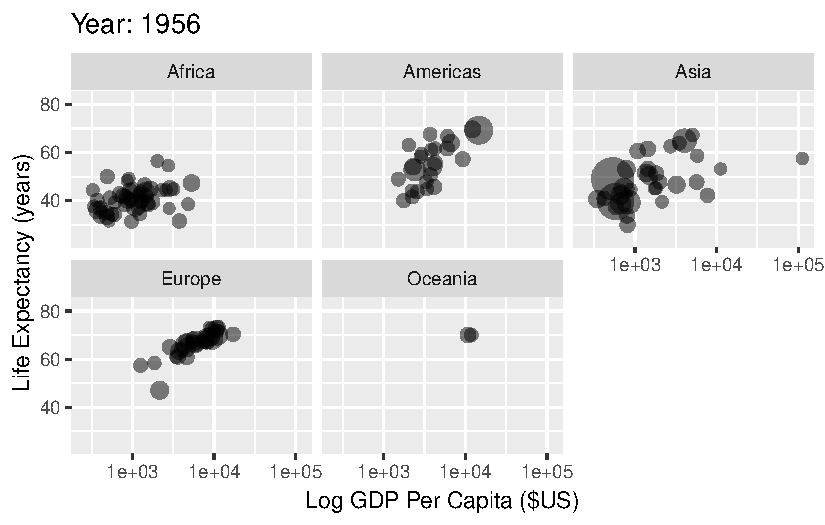
\includegraphics{index_files/figure-pdf/fig-anim-lifegdp-8.pdf}

}

\caption{\label{fig-anim-lifegdp-8}Life expectancy and GDP by country}

\end{figure}

\begin{figure}

{\centering 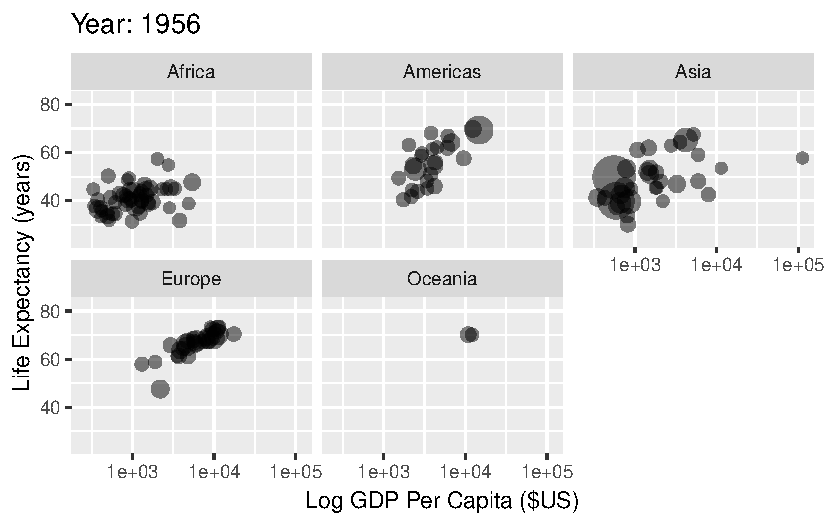
\includegraphics{index_files/figure-pdf/fig-anim-lifegdp-9.pdf}

}

\caption{\label{fig-anim-lifegdp-9}Life expectancy and GDP by country}

\end{figure}

\begin{figure}

{\centering 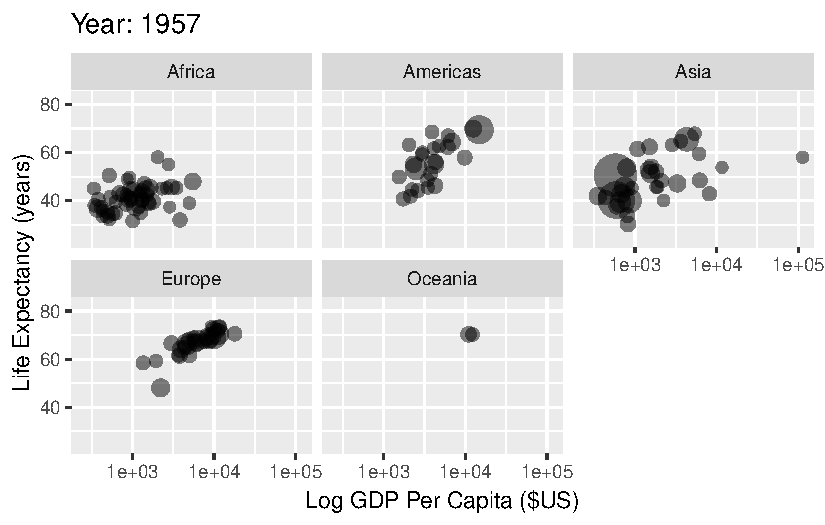
\includegraphics{index_files/figure-pdf/fig-anim-lifegdp-10.pdf}

}

\caption{\label{fig-anim-lifegdp-10}Life expectancy and GDP by country}

\end{figure}

\begin{figure}

{\centering 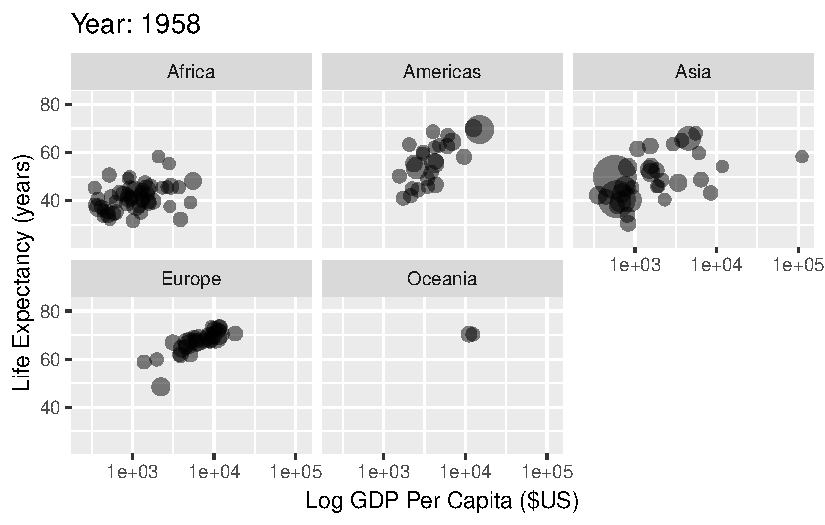
\includegraphics{index_files/figure-pdf/fig-anim-lifegdp-11.pdf}

}

\caption{\label{fig-anim-lifegdp-11}Life expectancy and GDP by country}

\end{figure}

\begin{figure}

{\centering 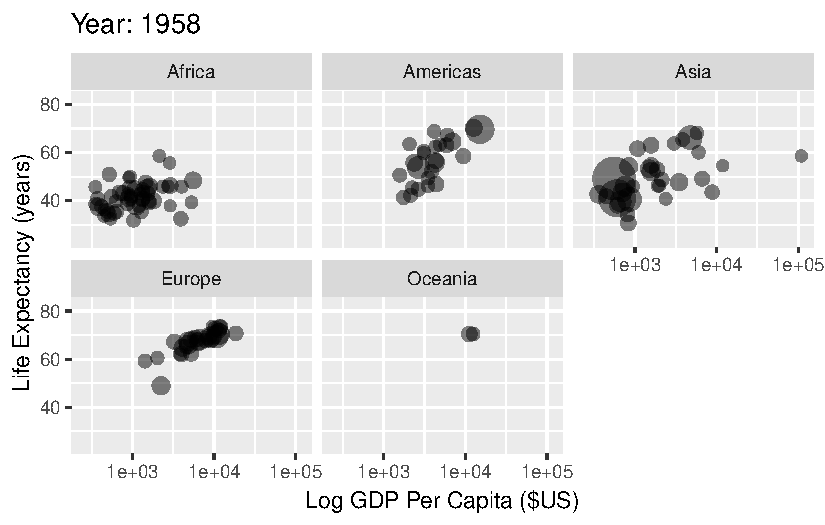
\includegraphics{index_files/figure-pdf/fig-anim-lifegdp-12.pdf}

}

\caption{\label{fig-anim-lifegdp-12}Life expectancy and GDP by country}

\end{figure}

\begin{figure}

{\centering 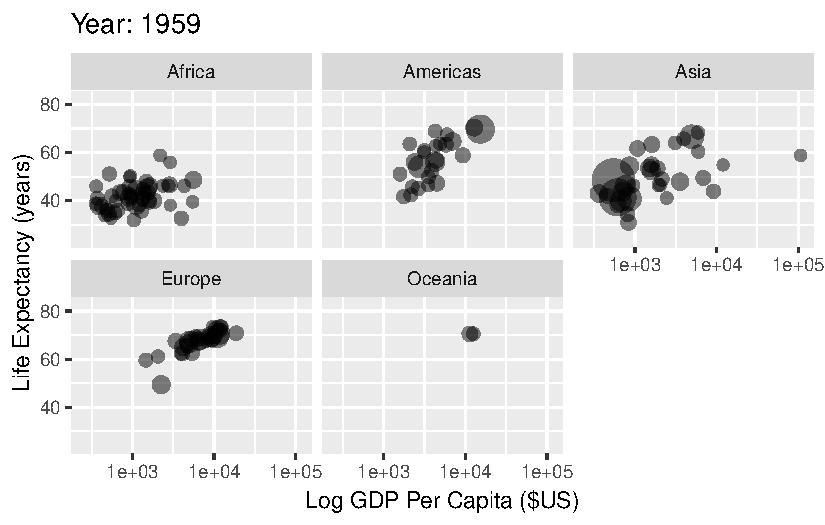
\includegraphics{index_files/figure-pdf/fig-anim-lifegdp-13.pdf}

}

\caption{\label{fig-anim-lifegdp-13}Life expectancy and GDP by country}

\end{figure}

\begin{figure}

{\centering 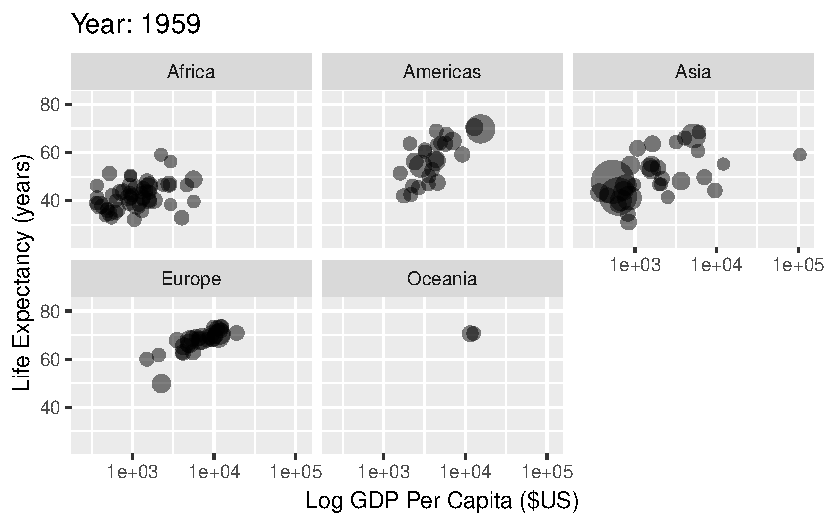
\includegraphics{index_files/figure-pdf/fig-anim-lifegdp-14.pdf}

}

\caption{\label{fig-anim-lifegdp-14}Life expectancy and GDP by country}

\end{figure}

\begin{figure}

{\centering 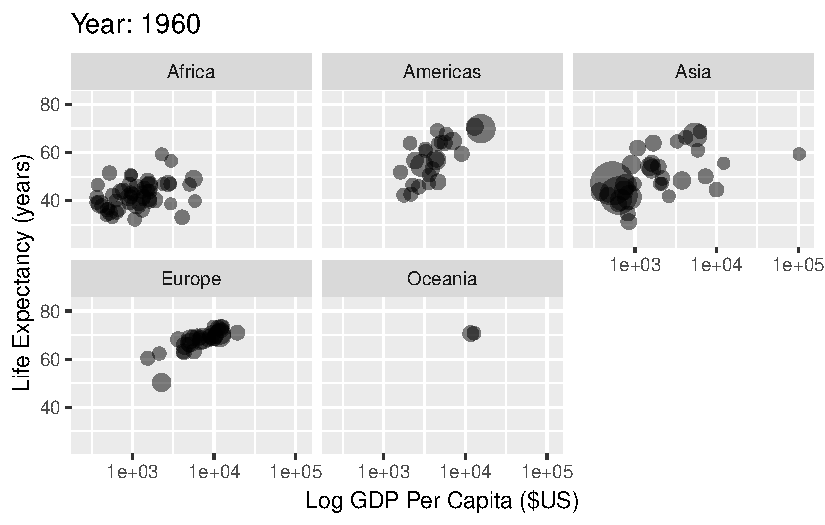
\includegraphics{index_files/figure-pdf/fig-anim-lifegdp-15.pdf}

}

\caption{\label{fig-anim-lifegdp-15}Life expectancy and GDP by country}

\end{figure}

\begin{figure}

{\centering 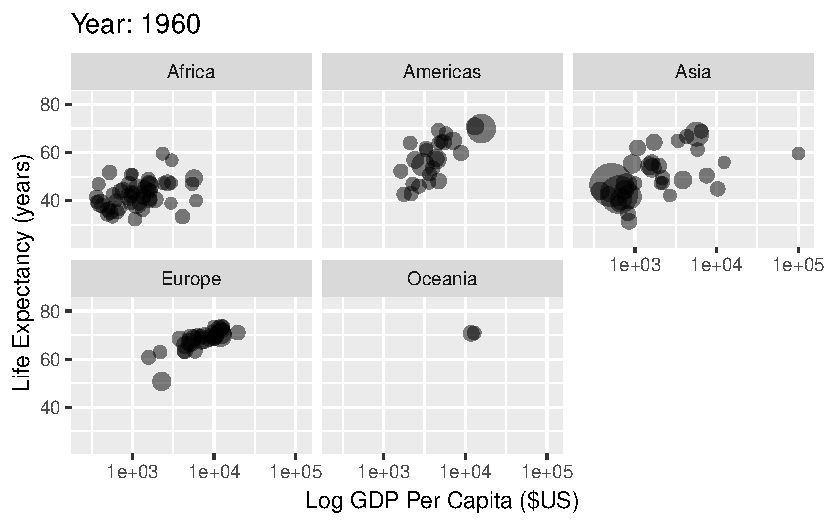
\includegraphics{index_files/figure-pdf/fig-anim-lifegdp-16.pdf}

}

\caption{\label{fig-anim-lifegdp-16}Life expectancy and GDP by country}

\end{figure}

\begin{figure}

{\centering 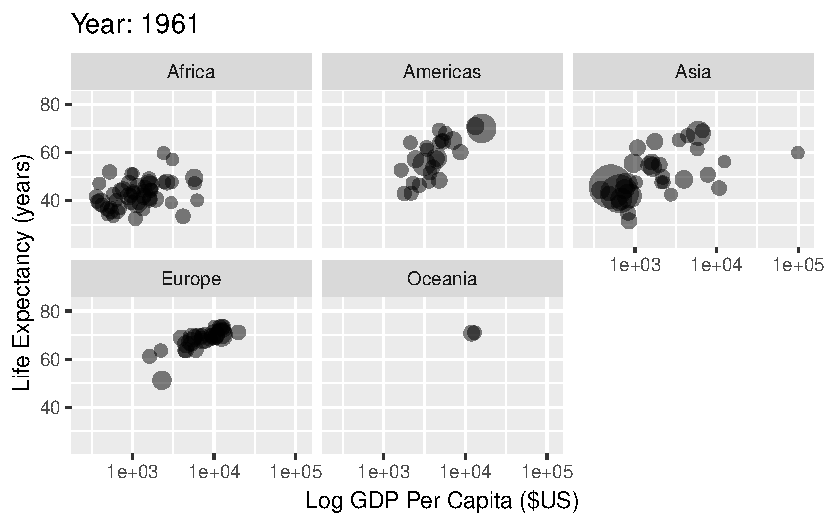
\includegraphics{index_files/figure-pdf/fig-anim-lifegdp-17.pdf}

}

\caption{\label{fig-anim-lifegdp-17}Life expectancy and GDP by country}

\end{figure}

\begin{figure}

{\centering 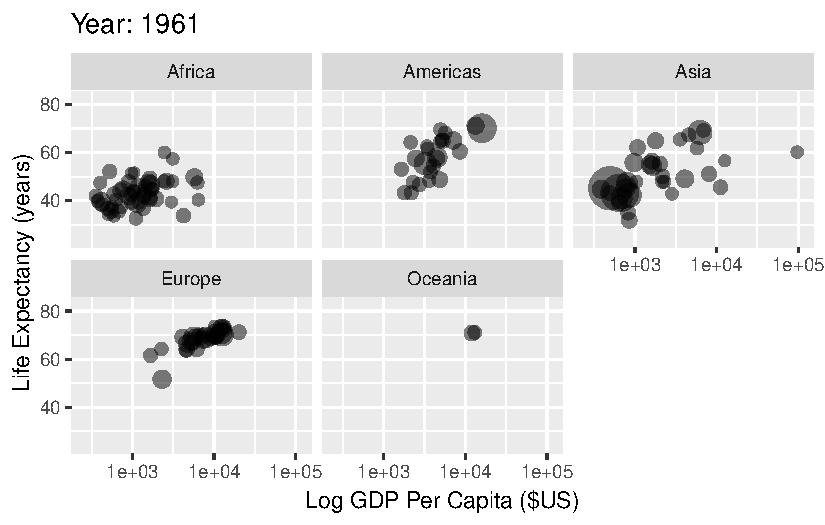
\includegraphics{index_files/figure-pdf/fig-anim-lifegdp-18.pdf}

}

\caption{\label{fig-anim-lifegdp-18}Life expectancy and GDP by country}

\end{figure}

\begin{figure}

{\centering 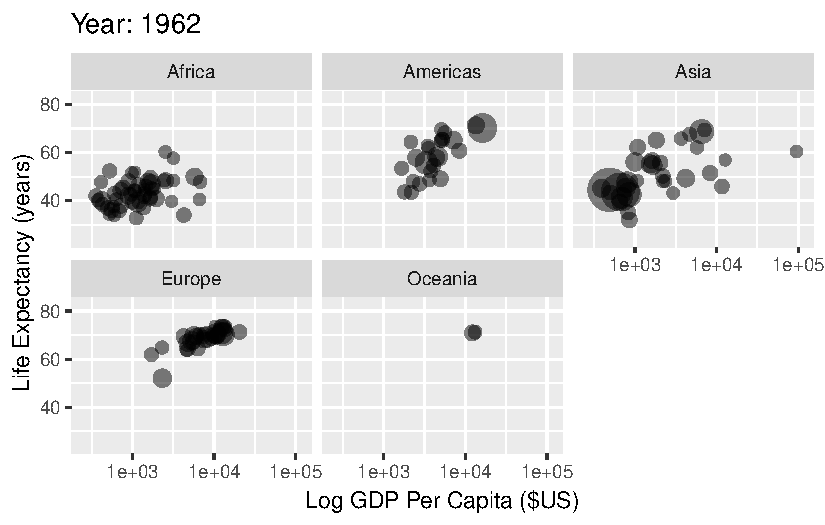
\includegraphics{index_files/figure-pdf/fig-anim-lifegdp-19.pdf}

}

\caption{\label{fig-anim-lifegdp-19}Life expectancy and GDP by country}

\end{figure}

\begin{figure}

{\centering 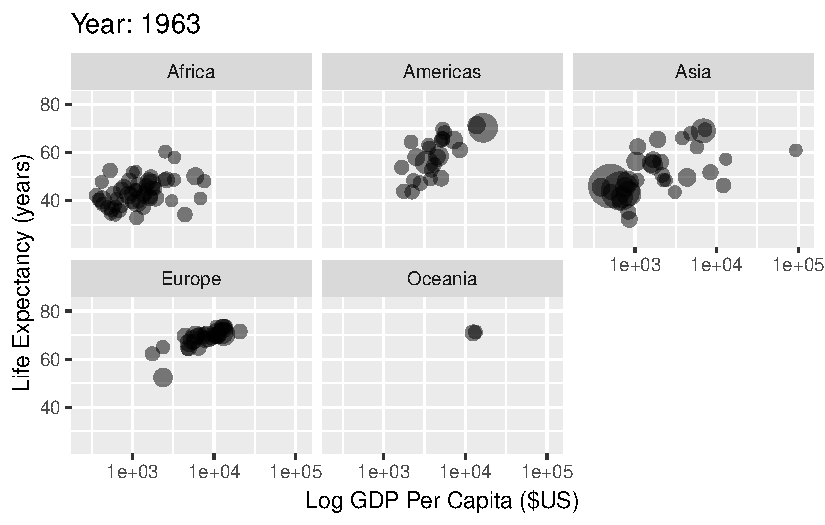
\includegraphics{index_files/figure-pdf/fig-anim-lifegdp-20.pdf}

}

\caption{\label{fig-anim-lifegdp-20}Life expectancy and GDP by country}

\end{figure}

\begin{figure}

{\centering 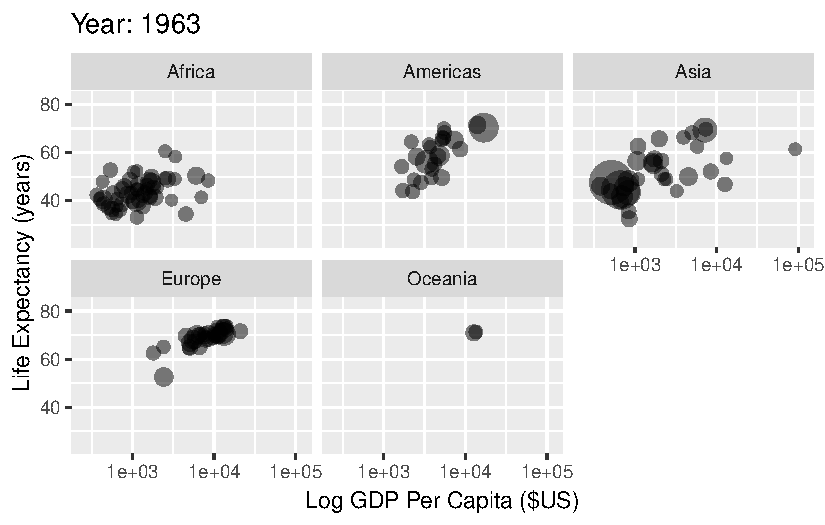
\includegraphics{index_files/figure-pdf/fig-anim-lifegdp-21.pdf}

}

\caption{\label{fig-anim-lifegdp-21}Life expectancy and GDP by country}

\end{figure}

\begin{figure}

{\centering 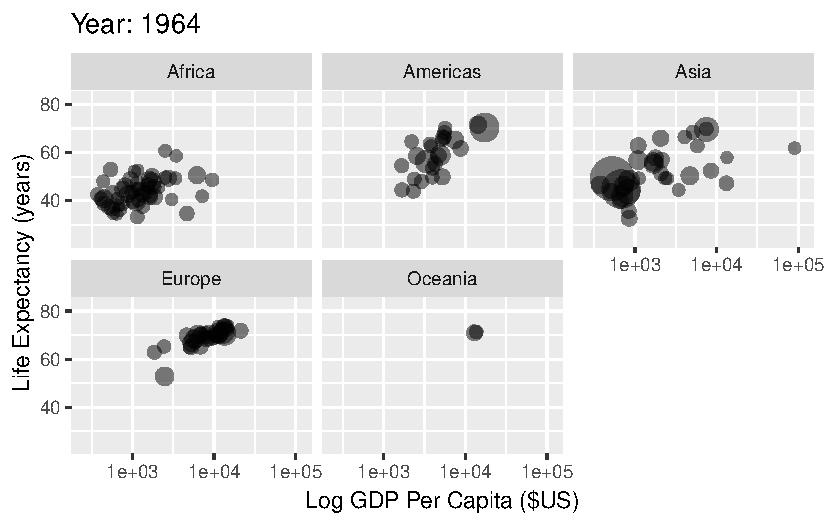
\includegraphics{index_files/figure-pdf/fig-anim-lifegdp-22.pdf}

}

\caption{\label{fig-anim-lifegdp-22}Life expectancy and GDP by country}

\end{figure}

\begin{figure}

{\centering 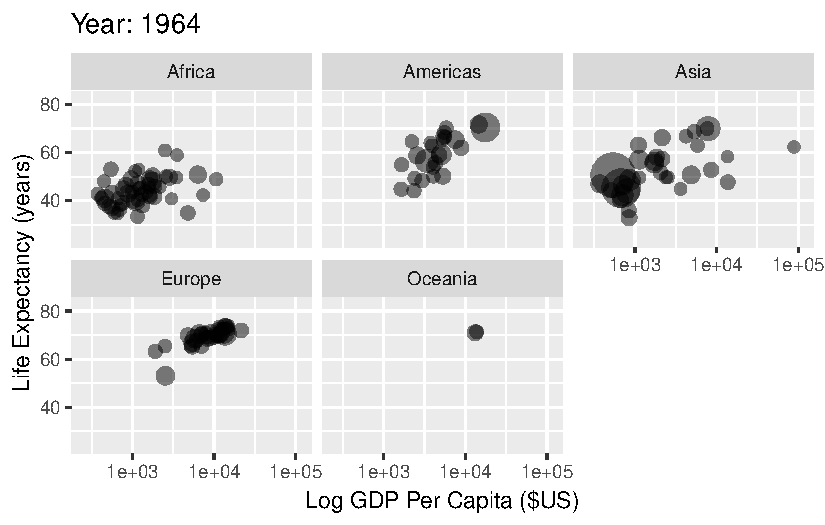
\includegraphics{index_files/figure-pdf/fig-anim-lifegdp-23.pdf}

}

\caption{\label{fig-anim-lifegdp-23}Life expectancy and GDP by country}

\end{figure}

\begin{figure}

{\centering 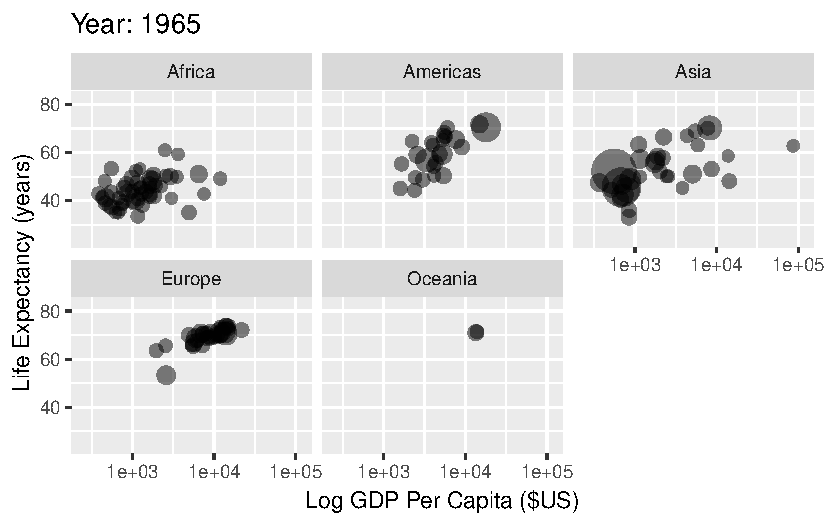
\includegraphics{index_files/figure-pdf/fig-anim-lifegdp-24.pdf}

}

\caption{\label{fig-anim-lifegdp-24}Life expectancy and GDP by country}

\end{figure}

\begin{figure}

{\centering 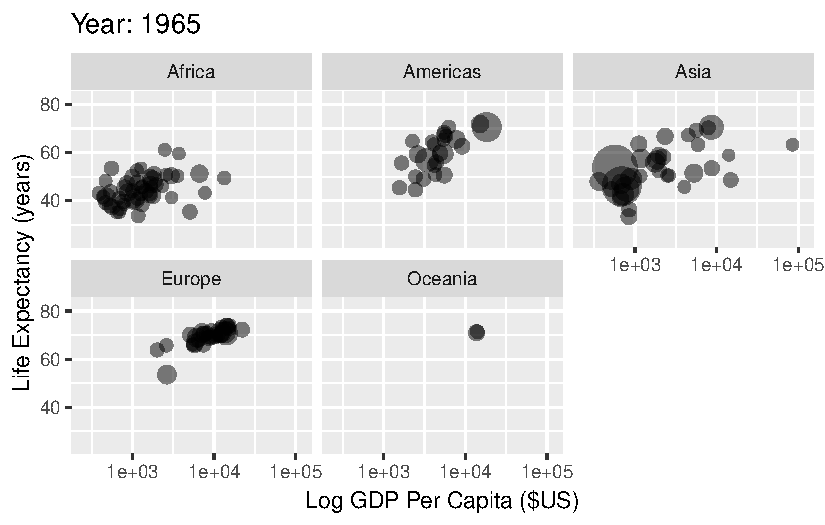
\includegraphics{index_files/figure-pdf/fig-anim-lifegdp-25.pdf}

}

\caption{\label{fig-anim-lifegdp-25}Life expectancy and GDP by country}

\end{figure}

\begin{figure}

{\centering 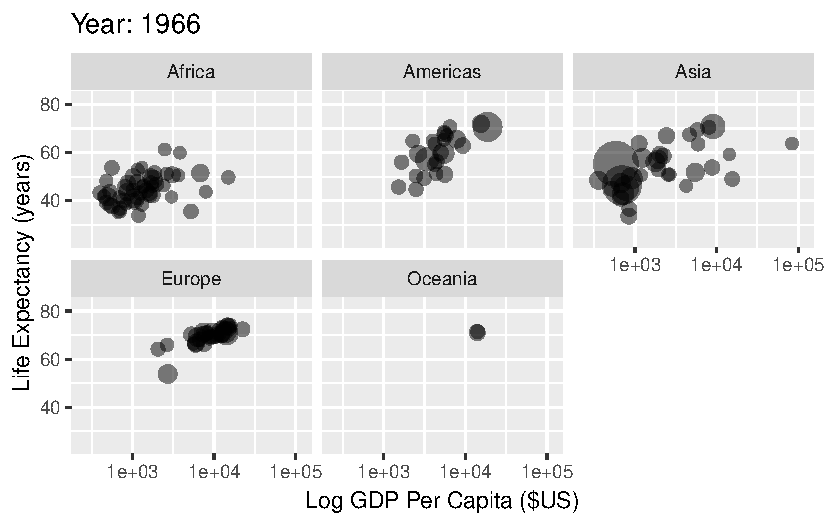
\includegraphics{index_files/figure-pdf/fig-anim-lifegdp-26.pdf}

}

\caption{\label{fig-anim-lifegdp-26}Life expectancy and GDP by country}

\end{figure}

\begin{figure}

{\centering 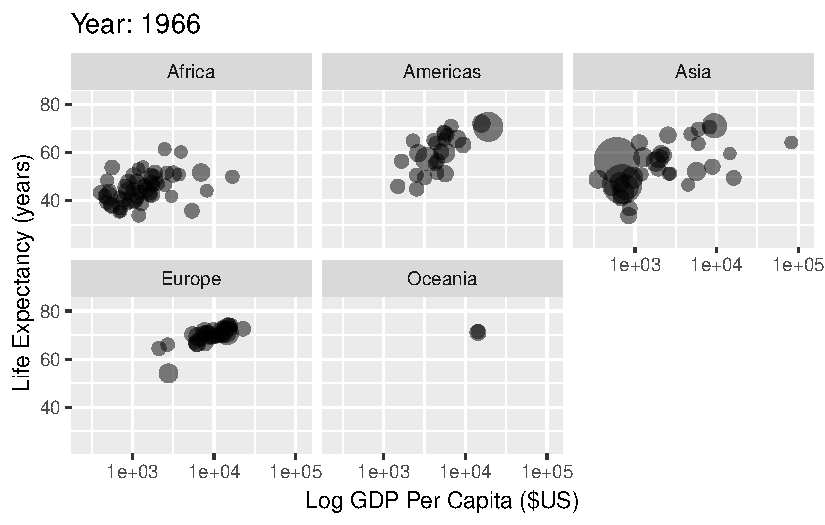
\includegraphics{index_files/figure-pdf/fig-anim-lifegdp-27.pdf}

}

\caption{\label{fig-anim-lifegdp-27}Life expectancy and GDP by country}

\end{figure}

\begin{figure}

{\centering 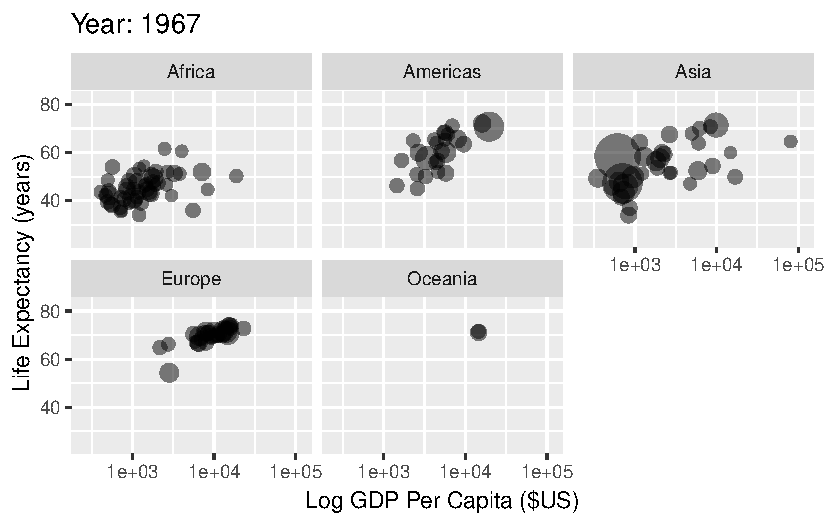
\includegraphics{index_files/figure-pdf/fig-anim-lifegdp-28.pdf}

}

\caption{\label{fig-anim-lifegdp-28}Life expectancy and GDP by country}

\end{figure}

\begin{figure}

{\centering 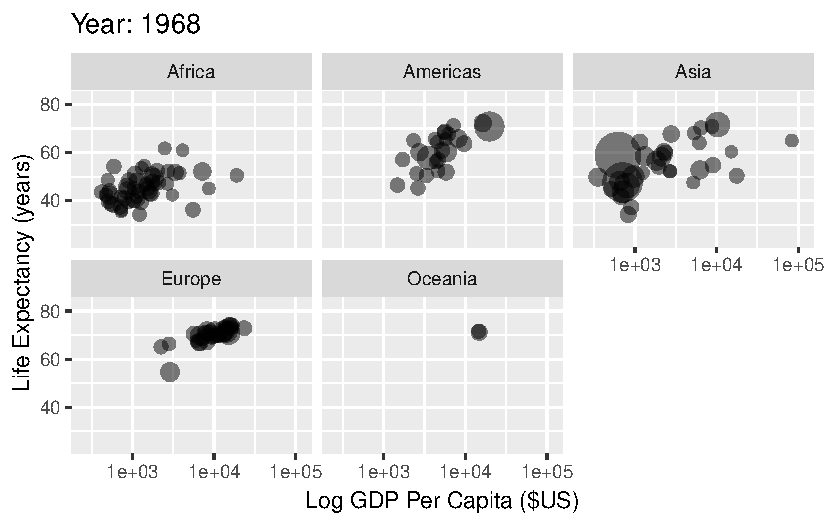
\includegraphics{index_files/figure-pdf/fig-anim-lifegdp-29.pdf}

}

\caption{\label{fig-anim-lifegdp-29}Life expectancy and GDP by country}

\end{figure}

\begin{figure}

{\centering 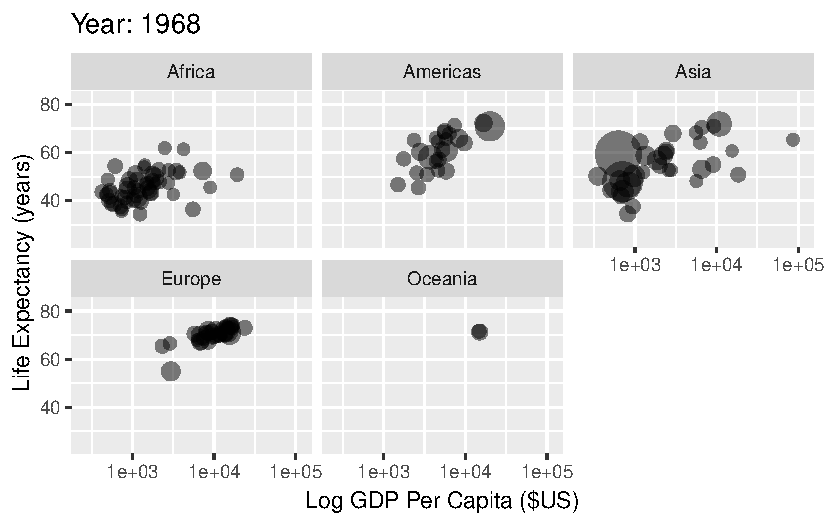
\includegraphics{index_files/figure-pdf/fig-anim-lifegdp-30.pdf}

}

\caption{\label{fig-anim-lifegdp-30}Life expectancy and GDP by country}

\end{figure}

\begin{figure}

{\centering 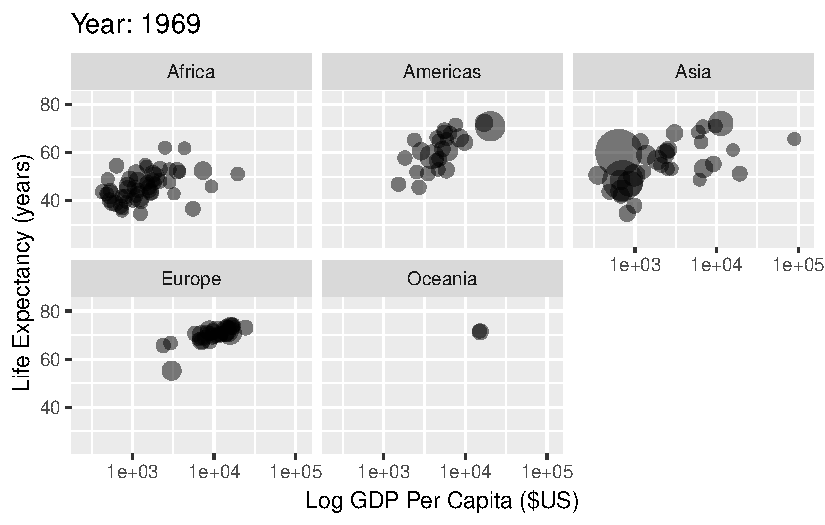
\includegraphics{index_files/figure-pdf/fig-anim-lifegdp-31.pdf}

}

\caption{\label{fig-anim-lifegdp-31}Life expectancy and GDP by country}

\end{figure}

\begin{figure}

{\centering 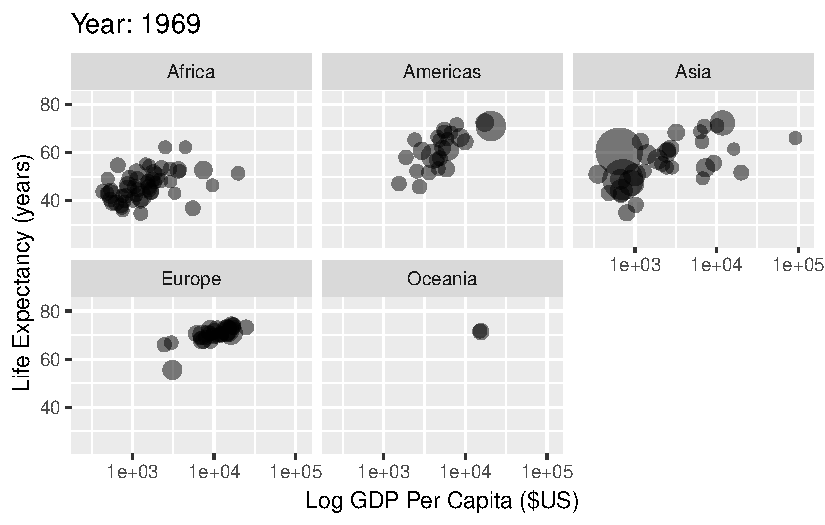
\includegraphics{index_files/figure-pdf/fig-anim-lifegdp-32.pdf}

}

\caption{\label{fig-anim-lifegdp-32}Life expectancy and GDP by country}

\end{figure}

\begin{figure}

{\centering 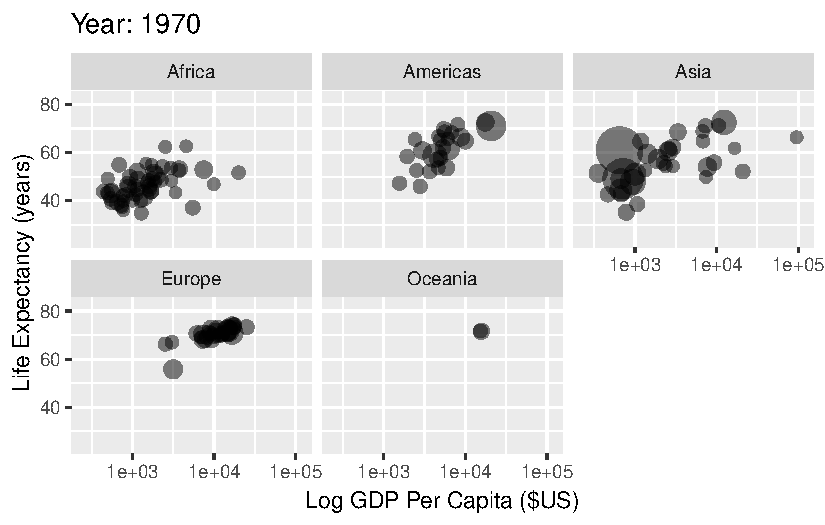
\includegraphics{index_files/figure-pdf/fig-anim-lifegdp-33.pdf}

}

\caption{\label{fig-anim-lifegdp-33}Life expectancy and GDP by country}

\end{figure}

\begin{figure}

{\centering 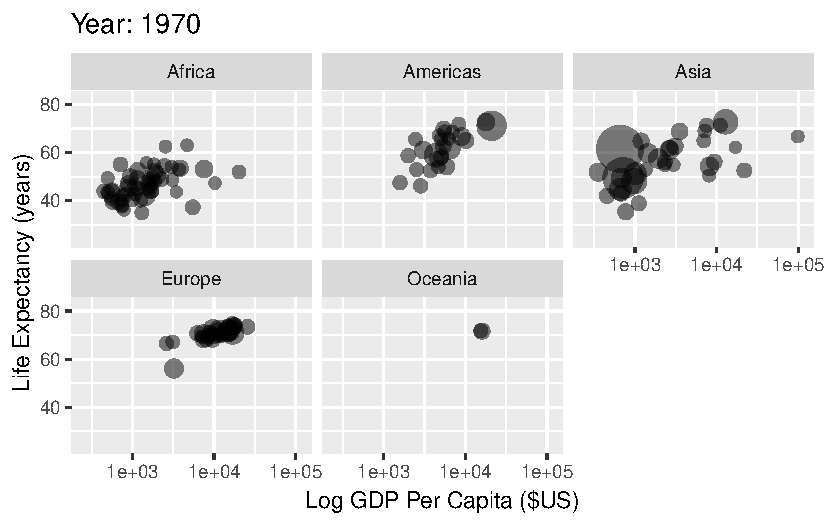
\includegraphics{index_files/figure-pdf/fig-anim-lifegdp-34.pdf}

}

\caption{\label{fig-anim-lifegdp-34}Life expectancy and GDP by country}

\end{figure}

\begin{figure}

{\centering 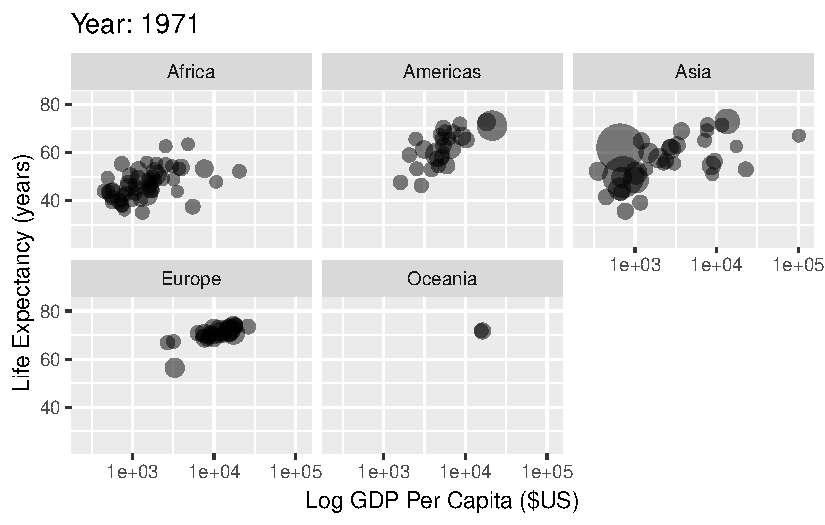
\includegraphics{index_files/figure-pdf/fig-anim-lifegdp-35.pdf}

}

\caption{\label{fig-anim-lifegdp-35}Life expectancy and GDP by country}

\end{figure}

\begin{figure}

{\centering 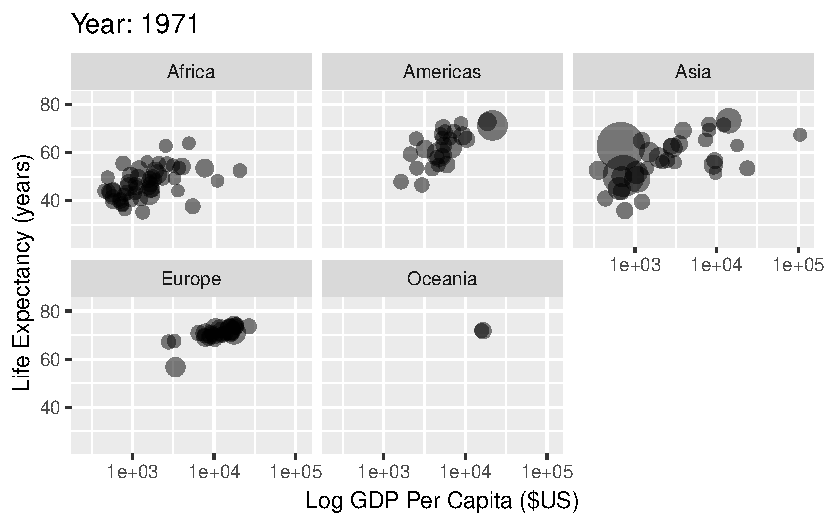
\includegraphics{index_files/figure-pdf/fig-anim-lifegdp-36.pdf}

}

\caption{\label{fig-anim-lifegdp-36}Life expectancy and GDP by country}

\end{figure}

\begin{figure}

{\centering 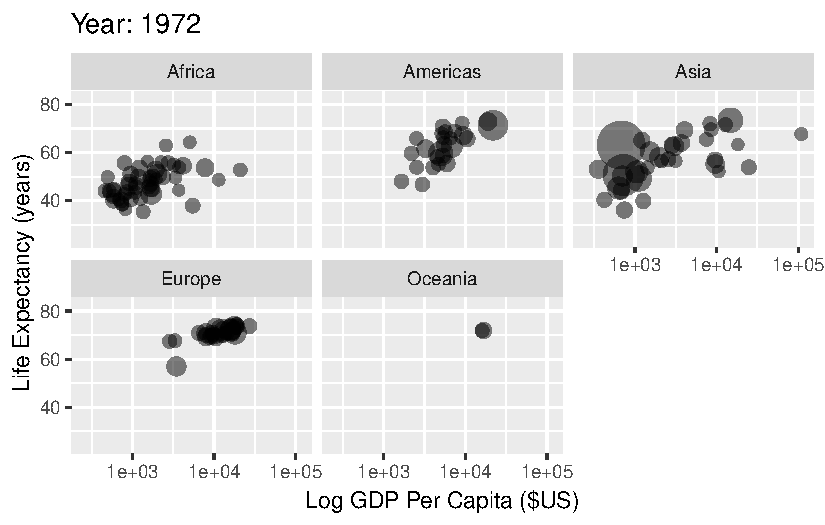
\includegraphics{index_files/figure-pdf/fig-anim-lifegdp-37.pdf}

}

\caption{\label{fig-anim-lifegdp-37}Life expectancy and GDP by country}

\end{figure}

\begin{figure}

{\centering 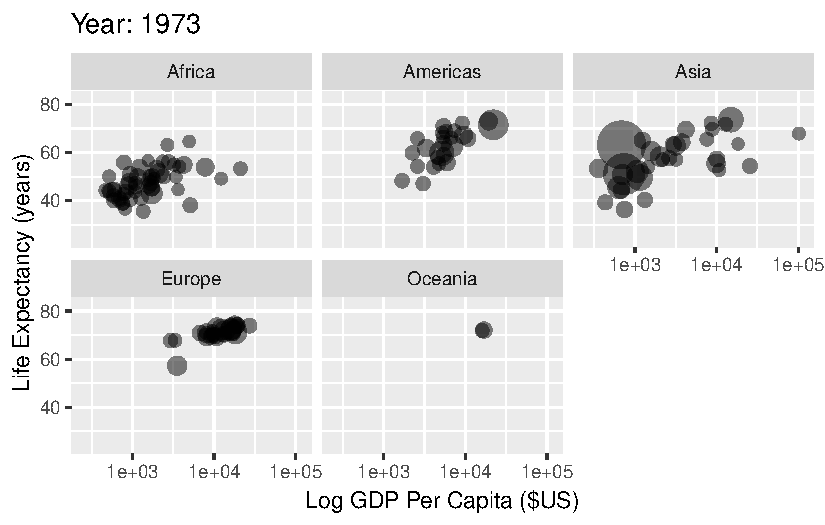
\includegraphics{index_files/figure-pdf/fig-anim-lifegdp-38.pdf}

}

\caption{\label{fig-anim-lifegdp-38}Life expectancy and GDP by country}

\end{figure}

\begin{figure}

{\centering 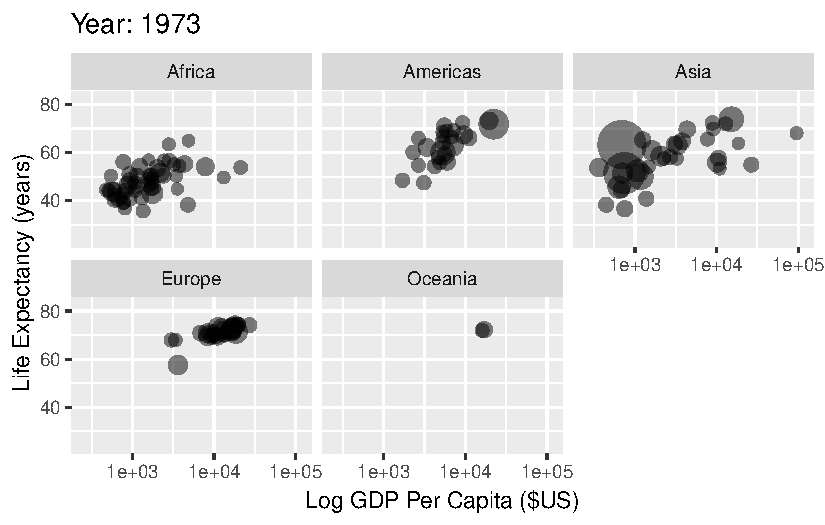
\includegraphics{index_files/figure-pdf/fig-anim-lifegdp-39.pdf}

}

\caption{\label{fig-anim-lifegdp-39}Life expectancy and GDP by country}

\end{figure}

\begin{figure}

{\centering 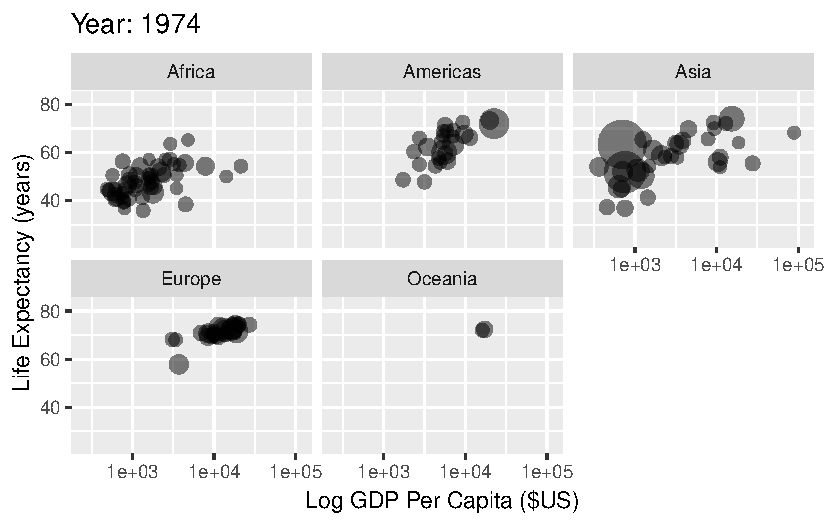
\includegraphics{index_files/figure-pdf/fig-anim-lifegdp-40.pdf}

}

\caption{\label{fig-anim-lifegdp-40}Life expectancy and GDP by country}

\end{figure}

\begin{figure}

{\centering 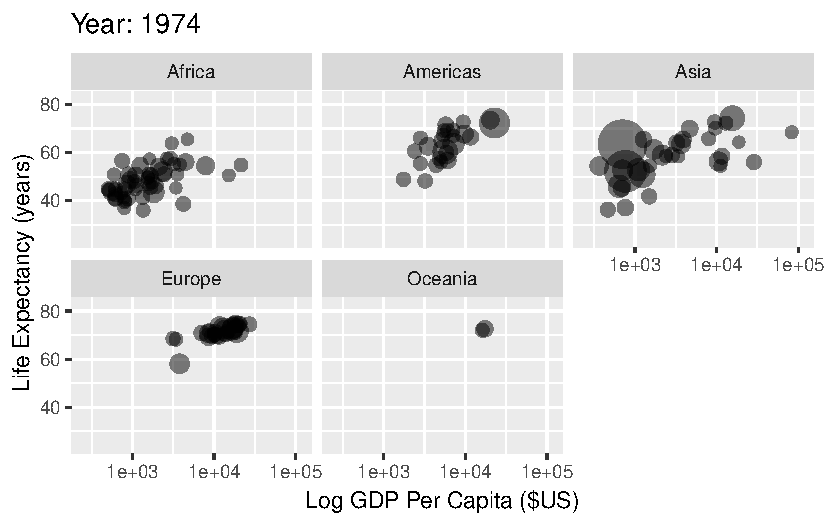
\includegraphics{index_files/figure-pdf/fig-anim-lifegdp-41.pdf}

}

\caption{\label{fig-anim-lifegdp-41}Life expectancy and GDP by country}

\end{figure}

\begin{figure}

{\centering 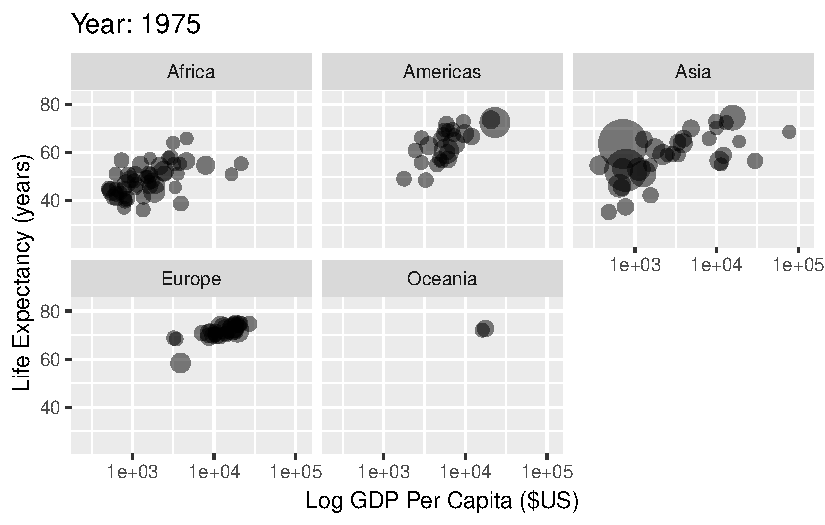
\includegraphics{index_files/figure-pdf/fig-anim-lifegdp-42.pdf}

}

\caption{\label{fig-anim-lifegdp-42}Life expectancy and GDP by country}

\end{figure}

\begin{figure}

{\centering 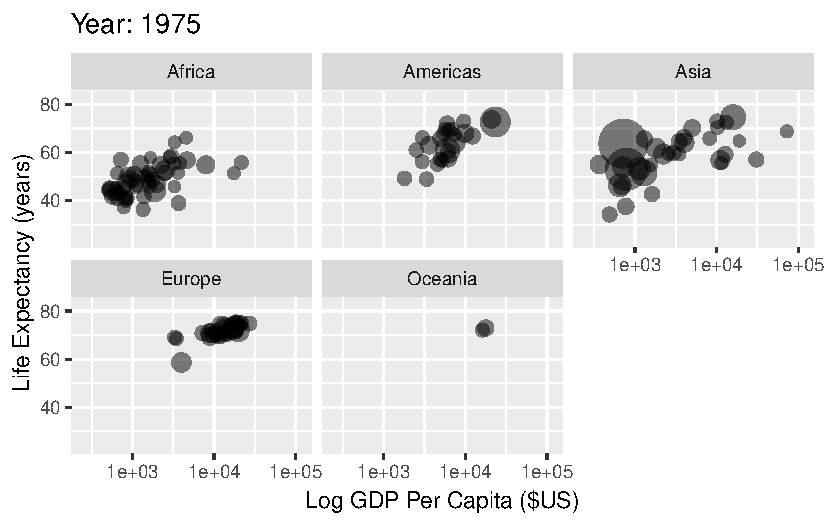
\includegraphics{index_files/figure-pdf/fig-anim-lifegdp-43.pdf}

}

\caption{\label{fig-anim-lifegdp-43}Life expectancy and GDP by country}

\end{figure}

\begin{figure}

{\centering 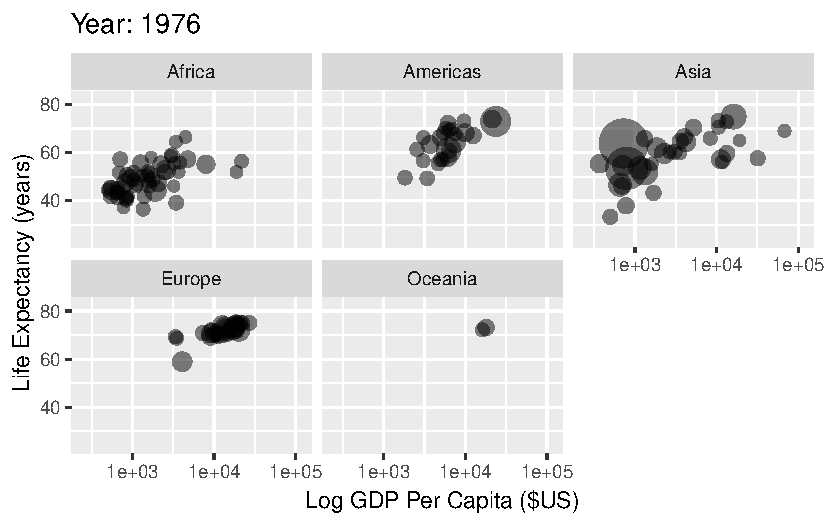
\includegraphics{index_files/figure-pdf/fig-anim-lifegdp-44.pdf}

}

\caption{\label{fig-anim-lifegdp-44}Life expectancy and GDP by country}

\end{figure}

\begin{figure}

{\centering 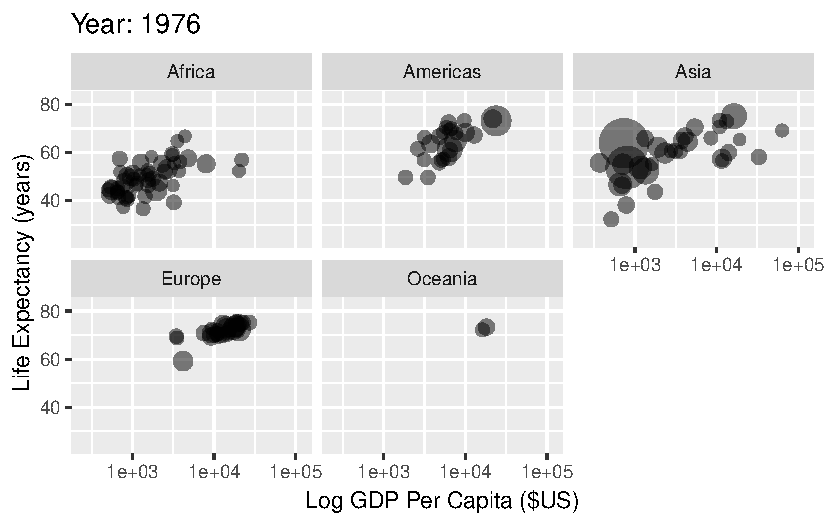
\includegraphics{index_files/figure-pdf/fig-anim-lifegdp-45.pdf}

}

\caption{\label{fig-anim-lifegdp-45}Life expectancy and GDP by country}

\end{figure}

\begin{figure}

{\centering 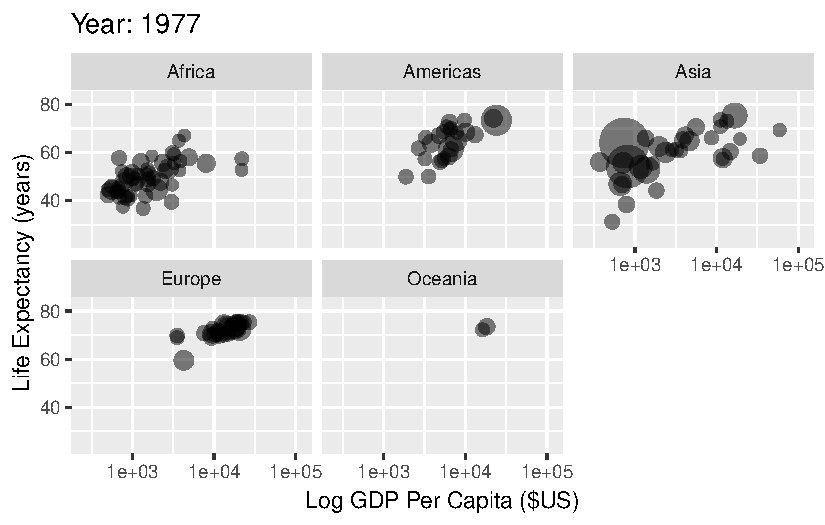
\includegraphics{index_files/figure-pdf/fig-anim-lifegdp-46.pdf}

}

\caption{\label{fig-anim-lifegdp-46}Life expectancy and GDP by country}

\end{figure}

\begin{figure}

{\centering 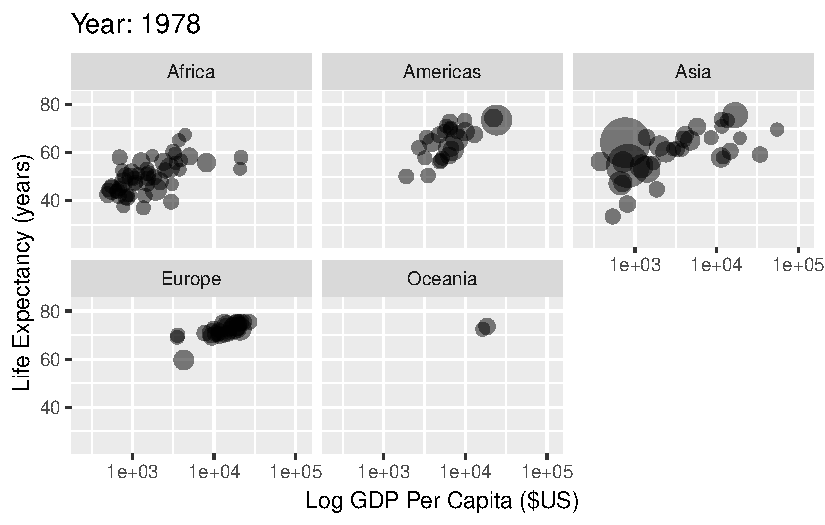
\includegraphics{index_files/figure-pdf/fig-anim-lifegdp-47.pdf}

}

\caption{\label{fig-anim-lifegdp-47}Life expectancy and GDP by country}

\end{figure}

\begin{figure}

{\centering 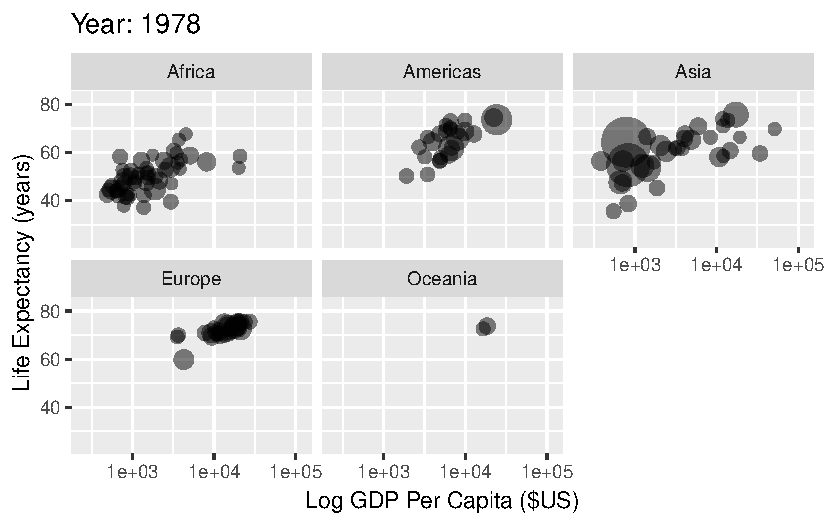
\includegraphics{index_files/figure-pdf/fig-anim-lifegdp-48.pdf}

}

\caption{\label{fig-anim-lifegdp-48}Life expectancy and GDP by country}

\end{figure}

\begin{figure}

{\centering \includegraphics{index_files/figure-pdf/fig-anim-lifegdp-49.pdf}

}

\caption{\label{fig-anim-lifegdp-49}Life expectancy and GDP by country}

\end{figure}

\begin{figure}

{\centering \includegraphics{index_files/figure-pdf/fig-anim-lifegdp-50.pdf}

}

\caption{\label{fig-anim-lifegdp-50}Life expectancy and GDP by country}

\end{figure}

\begin{figure}

{\centering \includegraphics{index_files/figure-pdf/fig-anim-lifegdp-51.pdf}

}

\caption{\label{fig-anim-lifegdp-51}Life expectancy and GDP by country}

\end{figure}

\begin{figure}

{\centering \includegraphics{index_files/figure-pdf/fig-anim-lifegdp-52.pdf}

}

\caption{\label{fig-anim-lifegdp-52}Life expectancy and GDP by country}

\end{figure}

\begin{figure}

{\centering \includegraphics{index_files/figure-pdf/fig-anim-lifegdp-53.pdf}

}

\caption{\label{fig-anim-lifegdp-53}Life expectancy and GDP by country}

\end{figure}

\begin{figure}

{\centering \includegraphics{index_files/figure-pdf/fig-anim-lifegdp-54.pdf}

}

\caption{\label{fig-anim-lifegdp-54}Life expectancy and GDP by country}

\end{figure}

\begin{figure}

{\centering \includegraphics{index_files/figure-pdf/fig-anim-lifegdp-55.pdf}

}

\caption{\label{fig-anim-lifegdp-55}Life expectancy and GDP by country}

\end{figure}

\begin{figure}

{\centering \includegraphics{index_files/figure-pdf/fig-anim-lifegdp-56.pdf}

}

\caption{\label{fig-anim-lifegdp-56}Life expectancy and GDP by country}

\end{figure}

\begin{figure}

{\centering \includegraphics{index_files/figure-pdf/fig-anim-lifegdp-57.pdf}

}

\caption{\label{fig-anim-lifegdp-57}Life expectancy and GDP by country}

\end{figure}

\begin{figure}

{\centering \includegraphics{index_files/figure-pdf/fig-anim-lifegdp-58.pdf}

}

\caption{\label{fig-anim-lifegdp-58}Life expectancy and GDP by country}

\end{figure}

\begin{figure}

{\centering \includegraphics{index_files/figure-pdf/fig-anim-lifegdp-59.pdf}

}

\caption{\label{fig-anim-lifegdp-59}Life expectancy and GDP by country}

\end{figure}

\begin{figure}

{\centering \includegraphics{index_files/figure-pdf/fig-anim-lifegdp-60.pdf}

}

\caption{\label{fig-anim-lifegdp-60}Life expectancy and GDP by country}

\end{figure}

\begin{figure}

{\centering \includegraphics{index_files/figure-pdf/fig-anim-lifegdp-61.pdf}

}

\caption{\label{fig-anim-lifegdp-61}Life expectancy and GDP by country}

\end{figure}

\begin{figure}

{\centering \includegraphics{index_files/figure-pdf/fig-anim-lifegdp-62.pdf}

}

\caption{\label{fig-anim-lifegdp-62}Life expectancy and GDP by country}

\end{figure}

\begin{figure}

{\centering \includegraphics{index_files/figure-pdf/fig-anim-lifegdp-63.pdf}

}

\caption{\label{fig-anim-lifegdp-63}Life expectancy and GDP by country}

\end{figure}

\begin{figure}

{\centering \includegraphics{index_files/figure-pdf/fig-anim-lifegdp-64.pdf}

}

\caption{\label{fig-anim-lifegdp-64}Life expectancy and GDP by country}

\end{figure}

\begin{figure}

{\centering \includegraphics{index_files/figure-pdf/fig-anim-lifegdp-65.pdf}

}

\caption{\label{fig-anim-lifegdp-65}Life expectancy and GDP by country}

\end{figure}

\begin{figure}

{\centering \includegraphics{index_files/figure-pdf/fig-anim-lifegdp-66.pdf}

}

\caption{\label{fig-anim-lifegdp-66}Life expectancy and GDP by country}

\end{figure}

\begin{figure}

{\centering \includegraphics{index_files/figure-pdf/fig-anim-lifegdp-67.pdf}

}

\caption{\label{fig-anim-lifegdp-67}Life expectancy and GDP by country}

\end{figure}

\begin{figure}

{\centering \includegraphics{index_files/figure-pdf/fig-anim-lifegdp-68.pdf}

}

\caption{\label{fig-anim-lifegdp-68}Life expectancy and GDP by country}

\end{figure}

\begin{figure}

{\centering \includegraphics{index_files/figure-pdf/fig-anim-lifegdp-69.pdf}

}

\caption{\label{fig-anim-lifegdp-69}Life expectancy and GDP by country}

\end{figure}

\begin{figure}

{\centering \includegraphics{index_files/figure-pdf/fig-anim-lifegdp-70.pdf}

}

\caption{\label{fig-anim-lifegdp-70}Life expectancy and GDP by country}

\end{figure}

\begin{figure}

{\centering \includegraphics{index_files/figure-pdf/fig-anim-lifegdp-71.pdf}

}

\caption{\label{fig-anim-lifegdp-71}Life expectancy and GDP by country}

\end{figure}

\begin{figure}

{\centering \includegraphics{index_files/figure-pdf/fig-anim-lifegdp-72.pdf}

}

\caption{\label{fig-anim-lifegdp-72}Life expectancy and GDP by country}

\end{figure}

\begin{figure}

{\centering \includegraphics{index_files/figure-pdf/fig-anim-lifegdp-73.pdf}

}

\caption{\label{fig-anim-lifegdp-73}Life expectancy and GDP by country}

\end{figure}

\begin{figure}

{\centering \includegraphics{index_files/figure-pdf/fig-anim-lifegdp-74.pdf}

}

\caption{\label{fig-anim-lifegdp-74}Life expectancy and GDP by country}

\end{figure}

\begin{figure}

{\centering \includegraphics{index_files/figure-pdf/fig-anim-lifegdp-75.pdf}

}

\caption{\label{fig-anim-lifegdp-75}Life expectancy and GDP by country}

\end{figure}

\begin{figure}

{\centering \includegraphics{index_files/figure-pdf/fig-anim-lifegdp-76.pdf}

}

\caption{\label{fig-anim-lifegdp-76}Life expectancy and GDP by country}

\end{figure}

\begin{figure}

{\centering \includegraphics{index_files/figure-pdf/fig-anim-lifegdp-77.pdf}

}

\caption{\label{fig-anim-lifegdp-77}Life expectancy and GDP by country}

\end{figure}

\begin{figure}

{\centering \includegraphics{index_files/figure-pdf/fig-anim-lifegdp-78.pdf}

}

\caption{\label{fig-anim-lifegdp-78}Life expectancy and GDP by country}

\end{figure}

\begin{figure}

{\centering \includegraphics{index_files/figure-pdf/fig-anim-lifegdp-79.pdf}

}

\caption{\label{fig-anim-lifegdp-79}Life expectancy and GDP by country}

\end{figure}

\begin{figure}

{\centering \includegraphics{index_files/figure-pdf/fig-anim-lifegdp-80.pdf}

}

\caption{\label{fig-anim-lifegdp-80}Life expectancy and GDP by country}

\end{figure}

\begin{figure}

{\centering \includegraphics{index_files/figure-pdf/fig-anim-lifegdp-81.pdf}

}

\caption{\label{fig-anim-lifegdp-81}Life expectancy and GDP by country}

\end{figure}

\begin{figure}

{\centering \includegraphics{index_files/figure-pdf/fig-anim-lifegdp-82.pdf}

}

\caption{\label{fig-anim-lifegdp-82}Life expectancy and GDP by country}

\end{figure}

\begin{figure}

{\centering \includegraphics{index_files/figure-pdf/fig-anim-lifegdp-83.pdf}

}

\caption{\label{fig-anim-lifegdp-83}Life expectancy and GDP by country}

\end{figure}

\begin{figure}

{\centering \includegraphics{index_files/figure-pdf/fig-anim-lifegdp-84.pdf}

}

\caption{\label{fig-anim-lifegdp-84}Life expectancy and GDP by country}

\end{figure}

\begin{figure}

{\centering \includegraphics{index_files/figure-pdf/fig-anim-lifegdp-85.pdf}

}

\caption{\label{fig-anim-lifegdp-85}Life expectancy and GDP by country}

\end{figure}

\begin{figure}

{\centering \includegraphics{index_files/figure-pdf/fig-anim-lifegdp-86.pdf}

}

\caption{\label{fig-anim-lifegdp-86}Life expectancy and GDP by country}

\end{figure}

\begin{figure}

{\centering \includegraphics{index_files/figure-pdf/fig-anim-lifegdp-87.pdf}

}

\caption{\label{fig-anim-lifegdp-87}Life expectancy and GDP by country}

\end{figure}

\begin{figure}

{\centering \includegraphics{index_files/figure-pdf/fig-anim-lifegdp-88.pdf}

}

\caption{\label{fig-anim-lifegdp-88}Life expectancy and GDP by country}

\end{figure}

\begin{figure}

{\centering \includegraphics{index_files/figure-pdf/fig-anim-lifegdp-89.pdf}

}

\caption{\label{fig-anim-lifegdp-89}Life expectancy and GDP by country}

\end{figure}

\begin{figure}

{\centering \includegraphics{index_files/figure-pdf/fig-anim-lifegdp-90.pdf}

}

\caption{\label{fig-anim-lifegdp-90}Life expectancy and GDP by country}

\end{figure}

\begin{figure}

{\centering \includegraphics{index_files/figure-pdf/fig-anim-lifegdp-91.pdf}

}

\caption{\label{fig-anim-lifegdp-91}Life expectancy and GDP by country}

\end{figure}

\begin{figure}

{\centering \includegraphics{index_files/figure-pdf/fig-anim-lifegdp-92.pdf}

}

\caption{\label{fig-anim-lifegdp-92}Life expectancy and GDP by country}

\end{figure}

\begin{figure}

{\centering \includegraphics{index_files/figure-pdf/fig-anim-lifegdp-93.pdf}

}

\caption{\label{fig-anim-lifegdp-93}Life expectancy and GDP by country}

\end{figure}

\begin{figure}

{\centering \includegraphics{index_files/figure-pdf/fig-anim-lifegdp-94.pdf}

}

\caption{\label{fig-anim-lifegdp-94}Life expectancy and GDP by country}

\end{figure}

\begin{figure}

{\centering \includegraphics{index_files/figure-pdf/fig-anim-lifegdp-95.pdf}

}

\caption{\label{fig-anim-lifegdp-95}Life expectancy and GDP by country}

\end{figure}

\begin{figure}

{\centering \includegraphics{index_files/figure-pdf/fig-anim-lifegdp-96.pdf}

}

\caption{\label{fig-anim-lifegdp-96}Life expectancy and GDP by country}

\end{figure}

\begin{figure}

{\centering \includegraphics{index_files/figure-pdf/fig-anim-lifegdp-97.pdf}

}

\caption{\label{fig-anim-lifegdp-97}Life expectancy and GDP by country}

\end{figure}

\begin{figure}

{\centering \includegraphics{index_files/figure-pdf/fig-anim-lifegdp-98.pdf}

}

\caption{\label{fig-anim-lifegdp-98}Life expectancy and GDP by country}

\end{figure}

\begin{figure}

{\centering \includegraphics{index_files/figure-pdf/fig-anim-lifegdp-99.pdf}

}

\caption{\label{fig-anim-lifegdp-99}Life expectancy and GDP by country}

\end{figure}

\begin{figure}

{\centering \includegraphics{index_files/figure-pdf/fig-anim-lifegdp-100.pdf}

}

\caption{\label{fig-anim-lifegdp-100}Life expectancy and GDP by country}

\end{figure}

But conditional on a relatively high life expectancy, the link between
economic performance and life expectancy isn't so clear. The U.S. is a
good example. In \textbf{?@fig-anim-country}, we focus specifically on
G7 countries and highlight the U.S., where we see that the U.S. life
expectancy begins to flatten while GDP per capita begins to outgrow
those of other G7 countries.

\begin{figure}

{\centering \includegraphics{index_files/figure-pdf/fig-anim-country-1.pdf}

}

\caption{\label{fig-anim-country-1}Life expectancy and GDP by country}

\end{figure}

\begin{figure}

{\centering \includegraphics{index_files/figure-pdf/fig-anim-country-2.pdf}

}

\caption{\label{fig-anim-country-2}Life expectancy and GDP by country}

\end{figure}

\begin{figure}

{\centering \includegraphics{index_files/figure-pdf/fig-anim-country-3.pdf}

}

\caption{\label{fig-anim-country-3}Life expectancy and GDP by country}

\end{figure}

\begin{figure}

{\centering \includegraphics{index_files/figure-pdf/fig-anim-country-4.pdf}

}

\caption{\label{fig-anim-country-4}Life expectancy and GDP by country}

\end{figure}

\begin{figure}

{\centering \includegraphics{index_files/figure-pdf/fig-anim-country-5.pdf}

}

\caption{\label{fig-anim-country-5}Life expectancy and GDP by country}

\end{figure}

\begin{figure}

{\centering \includegraphics{index_files/figure-pdf/fig-anim-country-6.pdf}

}

\caption{\label{fig-anim-country-6}Life expectancy and GDP by country}

\end{figure}

\begin{figure}

{\centering \includegraphics{index_files/figure-pdf/fig-anim-country-7.pdf}

}

\caption{\label{fig-anim-country-7}Life expectancy and GDP by country}

\end{figure}

\begin{figure}

{\centering \includegraphics{index_files/figure-pdf/fig-anim-country-8.pdf}

}

\caption{\label{fig-anim-country-8}Life expectancy and GDP by country}

\end{figure}

\begin{figure}

{\centering \includegraphics{index_files/figure-pdf/fig-anim-country-9.pdf}

}

\caption{\label{fig-anim-country-9}Life expectancy and GDP by country}

\end{figure}

\begin{figure}

{\centering \includegraphics{index_files/figure-pdf/fig-anim-country-10.pdf}

}

\caption{\label{fig-anim-country-10}Life expectancy and GDP by country}

\end{figure}

\begin{figure}

{\centering \includegraphics{index_files/figure-pdf/fig-anim-country-11.pdf}

}

\caption{\label{fig-anim-country-11}Life expectancy and GDP by country}

\end{figure}

\begin{figure}

{\centering \includegraphics{index_files/figure-pdf/fig-anim-country-12.pdf}

}

\caption{\label{fig-anim-country-12}Life expectancy and GDP by country}

\end{figure}

\begin{figure}

{\centering \includegraphics{index_files/figure-pdf/fig-anim-country-13.pdf}

}

\caption{\label{fig-anim-country-13}Life expectancy and GDP by country}

\end{figure}

\begin{figure}

{\centering \includegraphics{index_files/figure-pdf/fig-anim-country-14.pdf}

}

\caption{\label{fig-anim-country-14}Life expectancy and GDP by country}

\end{figure}

\begin{figure}

{\centering \includegraphics{index_files/figure-pdf/fig-anim-country-15.pdf}

}

\caption{\label{fig-anim-country-15}Life expectancy and GDP by country}

\end{figure}

\begin{figure}

{\centering \includegraphics{index_files/figure-pdf/fig-anim-country-16.pdf}

}

\caption{\label{fig-anim-country-16}Life expectancy and GDP by country}

\end{figure}

\begin{figure}

{\centering \includegraphics{index_files/figure-pdf/fig-anim-country-17.pdf}

}

\caption{\label{fig-anim-country-17}Life expectancy and GDP by country}

\end{figure}

\begin{figure}

{\centering \includegraphics{index_files/figure-pdf/fig-anim-country-18.pdf}

}

\caption{\label{fig-anim-country-18}Life expectancy and GDP by country}

\end{figure}

\begin{figure}

{\centering \includegraphics{index_files/figure-pdf/fig-anim-country-19.pdf}

}

\caption{\label{fig-anim-country-19}Life expectancy and GDP by country}

\end{figure}

\begin{figure}

{\centering \includegraphics{index_files/figure-pdf/fig-anim-country-20.pdf}

}

\caption{\label{fig-anim-country-20}Life expectancy and GDP by country}

\end{figure}

\begin{figure}

{\centering \includegraphics{index_files/figure-pdf/fig-anim-country-21.pdf}

}

\caption{\label{fig-anim-country-21}Life expectancy and GDP by country}

\end{figure}

\begin{figure}

{\centering \includegraphics{index_files/figure-pdf/fig-anim-country-22.pdf}

}

\caption{\label{fig-anim-country-22}Life expectancy and GDP by country}

\end{figure}

\begin{figure}

{\centering \includegraphics{index_files/figure-pdf/fig-anim-country-23.pdf}

}

\caption{\label{fig-anim-country-23}Life expectancy and GDP by country}

\end{figure}

\begin{figure}

{\centering \includegraphics{index_files/figure-pdf/fig-anim-country-24.pdf}

}

\caption{\label{fig-anim-country-24}Life expectancy and GDP by country}

\end{figure}

\begin{figure}

{\centering \includegraphics{index_files/figure-pdf/fig-anim-country-25.pdf}

}

\caption{\label{fig-anim-country-25}Life expectancy and GDP by country}

\end{figure}

\begin{figure}

{\centering \includegraphics{index_files/figure-pdf/fig-anim-country-26.pdf}

}

\caption{\label{fig-anim-country-26}Life expectancy and GDP by country}

\end{figure}

\begin{figure}

{\centering \includegraphics{index_files/figure-pdf/fig-anim-country-27.pdf}

}

\caption{\label{fig-anim-country-27}Life expectancy and GDP by country}

\end{figure}

\begin{figure}

{\centering \includegraphics{index_files/figure-pdf/fig-anim-country-28.pdf}

}

\caption{\label{fig-anim-country-28}Life expectancy and GDP by country}

\end{figure}

\begin{figure}

{\centering \includegraphics{index_files/figure-pdf/fig-anim-country-29.pdf}

}

\caption{\label{fig-anim-country-29}Life expectancy and GDP by country}

\end{figure}

\begin{figure}

{\centering \includegraphics{index_files/figure-pdf/fig-anim-country-30.pdf}

}

\caption{\label{fig-anim-country-30}Life expectancy and GDP by country}

\end{figure}

\begin{figure}

{\centering \includegraphics{index_files/figure-pdf/fig-anim-country-31.pdf}

}

\caption{\label{fig-anim-country-31}Life expectancy and GDP by country}

\end{figure}

\begin{figure}

{\centering \includegraphics{index_files/figure-pdf/fig-anim-country-32.pdf}

}

\caption{\label{fig-anim-country-32}Life expectancy and GDP by country}

\end{figure}

\begin{figure}

{\centering \includegraphics{index_files/figure-pdf/fig-anim-country-33.pdf}

}

\caption{\label{fig-anim-country-33}Life expectancy and GDP by country}

\end{figure}

\begin{figure}

{\centering \includegraphics{index_files/figure-pdf/fig-anim-country-34.pdf}

}

\caption{\label{fig-anim-country-34}Life expectancy and GDP by country}

\end{figure}

\begin{figure}

{\centering \includegraphics{index_files/figure-pdf/fig-anim-country-35.pdf}

}

\caption{\label{fig-anim-country-35}Life expectancy and GDP by country}

\end{figure}

\begin{figure}

{\centering \includegraphics{index_files/figure-pdf/fig-anim-country-36.pdf}

}

\caption{\label{fig-anim-country-36}Life expectancy and GDP by country}

\end{figure}

\begin{figure}

{\centering \includegraphics{index_files/figure-pdf/fig-anim-country-37.pdf}

}

\caption{\label{fig-anim-country-37}Life expectancy and GDP by country}

\end{figure}

\begin{figure}

{\centering \includegraphics{index_files/figure-pdf/fig-anim-country-38.pdf}

}

\caption{\label{fig-anim-country-38}Life expectancy and GDP by country}

\end{figure}

\begin{figure}

{\centering \includegraphics{index_files/figure-pdf/fig-anim-country-39.pdf}

}

\caption{\label{fig-anim-country-39}Life expectancy and GDP by country}

\end{figure}

\begin{figure}

{\centering \includegraphics{index_files/figure-pdf/fig-anim-country-40.pdf}

}

\caption{\label{fig-anim-country-40}Life expectancy and GDP by country}

\end{figure}

\begin{figure}

{\centering \includegraphics{index_files/figure-pdf/fig-anim-country-41.pdf}

}

\caption{\label{fig-anim-country-41}Life expectancy and GDP by country}

\end{figure}

\begin{figure}

{\centering \includegraphics{index_files/figure-pdf/fig-anim-country-42.pdf}

}

\caption{\label{fig-anim-country-42}Life expectancy and GDP by country}

\end{figure}

\begin{figure}

{\centering \includegraphics{index_files/figure-pdf/fig-anim-country-43.pdf}

}

\caption{\label{fig-anim-country-43}Life expectancy and GDP by country}

\end{figure}

\begin{figure}

{\centering \includegraphics{index_files/figure-pdf/fig-anim-country-44.pdf}

}

\caption{\label{fig-anim-country-44}Life expectancy and GDP by country}

\end{figure}

\begin{figure}

{\centering \includegraphics{index_files/figure-pdf/fig-anim-country-45.pdf}

}

\caption{\label{fig-anim-country-45}Life expectancy and GDP by country}

\end{figure}

\begin{figure}

{\centering \includegraphics{index_files/figure-pdf/fig-anim-country-46.pdf}

}

\caption{\label{fig-anim-country-46}Life expectancy and GDP by country}

\end{figure}

\begin{figure}

{\centering \includegraphics{index_files/figure-pdf/fig-anim-country-47.pdf}

}

\caption{\label{fig-anim-country-47}Life expectancy and GDP by country}

\end{figure}

\begin{figure}

{\centering \includegraphics{index_files/figure-pdf/fig-anim-country-48.pdf}

}

\caption{\label{fig-anim-country-48}Life expectancy and GDP by country}

\end{figure}

\begin{figure}

{\centering \includegraphics{index_files/figure-pdf/fig-anim-country-49.pdf}

}

\caption{\label{fig-anim-country-49}Life expectancy and GDP by country}

\end{figure}

\begin{figure}

{\centering \includegraphics{index_files/figure-pdf/fig-anim-country-50.pdf}

}

\caption{\label{fig-anim-country-50}Life expectancy and GDP by country}

\end{figure}

\begin{figure}

{\centering \includegraphics{index_files/figure-pdf/fig-anim-country-51.pdf}

}

\caption{\label{fig-anim-country-51}Life expectancy and GDP by country}

\end{figure}

\begin{figure}

{\centering \includegraphics{index_files/figure-pdf/fig-anim-country-52.pdf}

}

\caption{\label{fig-anim-country-52}Life expectancy and GDP by country}

\end{figure}

\begin{figure}

{\centering \includegraphics{index_files/figure-pdf/fig-anim-country-53.pdf}

}

\caption{\label{fig-anim-country-53}Life expectancy and GDP by country}

\end{figure}

\begin{figure}

{\centering \includegraphics{index_files/figure-pdf/fig-anim-country-54.pdf}

}

\caption{\label{fig-anim-country-54}Life expectancy and GDP by country}

\end{figure}

\begin{figure}

{\centering \includegraphics{index_files/figure-pdf/fig-anim-country-55.pdf}

}

\caption{\label{fig-anim-country-55}Life expectancy and GDP by country}

\end{figure}

\begin{figure}

{\centering \includegraphics{index_files/figure-pdf/fig-anim-country-56.pdf}

}

\caption{\label{fig-anim-country-56}Life expectancy and GDP by country}

\end{figure}

\begin{figure}

{\centering \includegraphics{index_files/figure-pdf/fig-anim-country-57.pdf}

}

\caption{\label{fig-anim-country-57}Life expectancy and GDP by country}

\end{figure}

\begin{figure}

{\centering \includegraphics{index_files/figure-pdf/fig-anim-country-58.pdf}

}

\caption{\label{fig-anim-country-58}Life expectancy and GDP by country}

\end{figure}

\begin{figure}

{\centering \includegraphics{index_files/figure-pdf/fig-anim-country-59.pdf}

}

\caption{\label{fig-anim-country-59}Life expectancy and GDP by country}

\end{figure}

\begin{figure}

{\centering \includegraphics{index_files/figure-pdf/fig-anim-country-60.pdf}

}

\caption{\label{fig-anim-country-60}Life expectancy and GDP by country}

\end{figure}

\begin{figure}

{\centering \includegraphics{index_files/figure-pdf/fig-anim-country-61.pdf}

}

\caption{\label{fig-anim-country-61}Life expectancy and GDP by country}

\end{figure}

\begin{figure}

{\centering \includegraphics{index_files/figure-pdf/fig-anim-country-62.pdf}

}

\caption{\label{fig-anim-country-62}Life expectancy and GDP by country}

\end{figure}

\begin{figure}

{\centering \includegraphics{index_files/figure-pdf/fig-anim-country-63.pdf}

}

\caption{\label{fig-anim-country-63}Life expectancy and GDP by country}

\end{figure}

\begin{figure}

{\centering \includegraphics{index_files/figure-pdf/fig-anim-country-64.pdf}

}

\caption{\label{fig-anim-country-64}Life expectancy and GDP by country}

\end{figure}

\begin{figure}

{\centering \includegraphics{index_files/figure-pdf/fig-anim-country-65.pdf}

}

\caption{\label{fig-anim-country-65}Life expectancy and GDP by country}

\end{figure}

\begin{figure}

{\centering \includegraphics{index_files/figure-pdf/fig-anim-country-66.pdf}

}

\caption{\label{fig-anim-country-66}Life expectancy and GDP by country}

\end{figure}

\begin{figure}

{\centering \includegraphics{index_files/figure-pdf/fig-anim-country-67.pdf}

}

\caption{\label{fig-anim-country-67}Life expectancy and GDP by country}

\end{figure}

\begin{figure}

{\centering \includegraphics{index_files/figure-pdf/fig-anim-country-68.pdf}

}

\caption{\label{fig-anim-country-68}Life expectancy and GDP by country}

\end{figure}

\begin{figure}

{\centering \includegraphics{index_files/figure-pdf/fig-anim-country-69.pdf}

}

\caption{\label{fig-anim-country-69}Life expectancy and GDP by country}

\end{figure}

\begin{figure}

{\centering \includegraphics{index_files/figure-pdf/fig-anim-country-70.pdf}

}

\caption{\label{fig-anim-country-70}Life expectancy and GDP by country}

\end{figure}

\begin{figure}

{\centering \includegraphics{index_files/figure-pdf/fig-anim-country-71.pdf}

}

\caption{\label{fig-anim-country-71}Life expectancy and GDP by country}

\end{figure}

\begin{figure}

{\centering \includegraphics{index_files/figure-pdf/fig-anim-country-72.pdf}

}

\caption{\label{fig-anim-country-72}Life expectancy and GDP by country}

\end{figure}

\begin{figure}

{\centering \includegraphics{index_files/figure-pdf/fig-anim-country-73.pdf}

}

\caption{\label{fig-anim-country-73}Life expectancy and GDP by country}

\end{figure}

\begin{figure}

{\centering \includegraphics{index_files/figure-pdf/fig-anim-country-74.pdf}

}

\caption{\label{fig-anim-country-74}Life expectancy and GDP by country}

\end{figure}

\begin{figure}

{\centering \includegraphics{index_files/figure-pdf/fig-anim-country-75.pdf}

}

\caption{\label{fig-anim-country-75}Life expectancy and GDP by country}

\end{figure}

\begin{figure}

{\centering \includegraphics{index_files/figure-pdf/fig-anim-country-76.pdf}

}

\caption{\label{fig-anim-country-76}Life expectancy and GDP by country}

\end{figure}

\begin{figure}

{\centering \includegraphics{index_files/figure-pdf/fig-anim-country-77.pdf}

}

\caption{\label{fig-anim-country-77}Life expectancy and GDP by country}

\end{figure}

\begin{figure}

{\centering \includegraphics{index_files/figure-pdf/fig-anim-country-78.pdf}

}

\caption{\label{fig-anim-country-78}Life expectancy and GDP by country}

\end{figure}

\begin{figure}

{\centering \includegraphics{index_files/figure-pdf/fig-anim-country-79.pdf}

}

\caption{\label{fig-anim-country-79}Life expectancy and GDP by country}

\end{figure}

\begin{figure}

{\centering \includegraphics{index_files/figure-pdf/fig-anim-country-80.pdf}

}

\caption{\label{fig-anim-country-80}Life expectancy and GDP by country}

\end{figure}

\begin{figure}

{\centering \includegraphics{index_files/figure-pdf/fig-anim-country-81.pdf}

}

\caption{\label{fig-anim-country-81}Life expectancy and GDP by country}

\end{figure}

\begin{figure}

{\centering \includegraphics{index_files/figure-pdf/fig-anim-country-82.pdf}

}

\caption{\label{fig-anim-country-82}Life expectancy and GDP by country}

\end{figure}

\begin{figure}

{\centering \includegraphics{index_files/figure-pdf/fig-anim-country-83.pdf}

}

\caption{\label{fig-anim-country-83}Life expectancy and GDP by country}

\end{figure}

\begin{figure}

{\centering \includegraphics{index_files/figure-pdf/fig-anim-country-84.pdf}

}

\caption{\label{fig-anim-country-84}Life expectancy and GDP by country}

\end{figure}

\begin{figure}

{\centering \includegraphics{index_files/figure-pdf/fig-anim-country-85.pdf}

}

\caption{\label{fig-anim-country-85}Life expectancy and GDP by country}

\end{figure}

\begin{figure}

{\centering \includegraphics{index_files/figure-pdf/fig-anim-country-86.pdf}

}

\caption{\label{fig-anim-country-86}Life expectancy and GDP by country}

\end{figure}

\begin{figure}

{\centering \includegraphics{index_files/figure-pdf/fig-anim-country-87.pdf}

}

\caption{\label{fig-anim-country-87}Life expectancy and GDP by country}

\end{figure}

\begin{figure}

{\centering \includegraphics{index_files/figure-pdf/fig-anim-country-88.pdf}

}

\caption{\label{fig-anim-country-88}Life expectancy and GDP by country}

\end{figure}

\begin{figure}

{\centering \includegraphics{index_files/figure-pdf/fig-anim-country-89.pdf}

}

\caption{\label{fig-anim-country-89}Life expectancy and GDP by country}

\end{figure}

\begin{figure}

{\centering \includegraphics{index_files/figure-pdf/fig-anim-country-90.pdf}

}

\caption{\label{fig-anim-country-90}Life expectancy and GDP by country}

\end{figure}

\begin{figure}

{\centering \includegraphics{index_files/figure-pdf/fig-anim-country-91.pdf}

}

\caption{\label{fig-anim-country-91}Life expectancy and GDP by country}

\end{figure}

\begin{figure}

{\centering \includegraphics{index_files/figure-pdf/fig-anim-country-92.pdf}

}

\caption{\label{fig-anim-country-92}Life expectancy and GDP by country}

\end{figure}

\begin{figure}

{\centering \includegraphics{index_files/figure-pdf/fig-anim-country-93.pdf}

}

\caption{\label{fig-anim-country-93}Life expectancy and GDP by country}

\end{figure}

\begin{figure}

{\centering \includegraphics{index_files/figure-pdf/fig-anim-country-94.pdf}

}

\caption{\label{fig-anim-country-94}Life expectancy and GDP by country}

\end{figure}

\begin{figure}

{\centering \includegraphics{index_files/figure-pdf/fig-anim-country-95.pdf}

}

\caption{\label{fig-anim-country-95}Life expectancy and GDP by country}

\end{figure}

\begin{figure}

{\centering \includegraphics{index_files/figure-pdf/fig-anim-country-96.pdf}

}

\caption{\label{fig-anim-country-96}Life expectancy and GDP by country}

\end{figure}

\begin{figure}

{\centering \includegraphics{index_files/figure-pdf/fig-anim-country-97.pdf}

}

\caption{\label{fig-anim-country-97}Life expectancy and GDP by country}

\end{figure}

\begin{figure}

{\centering \includegraphics{index_files/figure-pdf/fig-anim-country-98.pdf}

}

\caption{\label{fig-anim-country-98}Life expectancy and GDP by country}

\end{figure}

\begin{figure}

{\centering \includegraphics{index_files/figure-pdf/fig-anim-country-99.pdf}

}

\caption{\label{fig-anim-country-99}Life expectancy and GDP by country}

\end{figure}

\begin{figure}

{\centering \includegraphics{index_files/figure-pdf/fig-anim-country-100.pdf}

}

\caption{\label{fig-anim-country-100}Life expectancy and GDP by country}

\end{figure}

\hypertarget{health-care-spending-and-outcomes}{%
\section*{Health Care Spending and
Outcomes}\label{health-care-spending-and-outcomes}}
\addcontentsline{toc}{section}{Health Care Spending and Outcomes}

\markright{Health Care Spending and Outcomes}

Of course, life expectancy is heavily influenced by things like car
accidents, guns, and other policy issues that are not necessarily
``health care'' related. As such, life expectancy is likely a poor
measure of the quality of a country's health care system. Still, despite
significantly larger health care expenditures, the U.S. continues to
underperform in more direct health care outcomes, like maternal
mortality and infant mortality presented in Figure~\ref{fig-mort}.
Around the mid-to-late 1980s, the U.S. begins spending substantially
more on health care as a percentage of GDP, while maternal and infant
mortality rates actually increase.

\begin{figure}

\begin{minipage}[t]{0.50\linewidth}

{\centering 

\raisebox{-\height}{

\includegraphics{figures/hcspend-maternal-mortality.gif}

}

}

\subcaption{\label{fig-maternal}maternal}
\end{minipage}%
%
\begin{minipage}[t]{0.50\linewidth}

{\centering 

\raisebox{-\height}{

\includegraphics{figures/hcspend-infant-mortality.gif}

}

}

\subcaption{\label{fig-infant}infant}
\end{minipage}%

\caption{\label{fig-mort}Maternal and infant mortality by country}

\end{figure}

Unfortunately, infant and maternal mortality are not the only measures
by which the U.S. health care system appears to be underperforming.
{``U.{S}. {Health} {Care} from a {Global} {Perspective}, 2019 {\textbar}
{Commonwealth} {Fund}''} (n.d.) provides a broader analysis of the U.S.
health care system in comparison to other high-income countries. The
2019 report (i.e., pre-Covid) highlights significant gaps in health
outcomes, access, and affordability in the U.S. compared to other
countries. Specifically, the U.S. ranks last among the 11 high-income
countries analyzed in terms of health outcomes, with higher rates of
mortality and morbidity from chronic diseases, such as heart disease,
diabetes, and cancer. Additionally, the U.S. has the highest rate of
mortality amenable to health care, suggesting that the health care
system is not functioning optimally. The report also finds that the U.S.
has the highest rate of adults who go without needed health care due to
cost, with one-third of adults reporting cost-related access problems.

That said, it is important to also note that the U.S. health care system
ranks among the best in the world in several key areas. One area in
which the U.S. excels is in the provision of specialized care,
particularly in the fields of cancer, heart disease, and stroke. The
U.S. has some of the highest survival rates for certain types of cancer,
such as breast and prostate cancer, and is a leader in the development
and use of advanced medical technologies, such as MRI and CT scans. The
U.S. also has some of the highest rates of bypass surgery and
angioplasty for heart disease, which can be life-saving interventions.

Another area of high-quality care in the U.S. is in the field of medical
research and innovation. The U.S. is home to many of the world's top
medical research institutions and is a leader in the development of new
drugs and medical devices. This innovation has led to significant
advances in the treatment of many diseases and has improved the quality
of life for millions of people.

This dichotomy of very good health care in some areas along side very
poor health care in other areas is reflective of what many believe to be
the true underlying problem with the U.S. health care system---access
to, and inequities in, health care. In many ways, we \emph{overprovide}
care to some people and \emph{underprovide} care to lots of other
people. We are particularly bad at helping the least healthy among us.
These issues are, of course, very closely related to other economic
problems and inequality in general.

\hypertarget{why-study-the-economics-of-health-care}{%
\section*{Why Study the Economics of Health
Care?}\label{why-study-the-economics-of-health-care}}
\addcontentsline{toc}{section}{Why Study the Economics of Health Care?}

\markright{Why Study the Economics of Health Care?}

Health care is a unique industry that presents several key economic
challenges. One key theoretical challenge to improving health care
(e.g., decreasing spending, improving quality, and reducing inequity) is
asymmetric information. In the context of health insurance, asymmetric
information describes the case in which patients may know more about
their health than insurance companies. This introduces the problem of
adverse selection, wherein patients with higher health care needs are
more likely to purchase insurance, leading to higher costs for insurers
and making it more difficult for insurers to design effective insurance
products. Insurers may have limited information about patients' health
status and risk, which can exacerbate adverse selection.

Asymmetric information also exists between patients and providers. Here,
patients often lack the knowledge and expertise to make informed
decisions about their health care, while physicians may have incentives
to recommend more expensive treatments. This can lead to overutilization
of health care services and higher costs for patients and insurers.
Additionally, patients may not have access to all of the relevant
information about their health care options, which can make it difficult
for them to make informed decisions about their care. These information
asymmetries can make it challenging to align incentives between patients
and physicians and can lead to inefficiencies in the market.

Health care also presents challenges due to unpredictable need and
product heterogeneity. Patients may require different types and levels
of care depending on their individual health needs, making it difficult
to standardize health care products and services. This can make it
challenging for patients to shop around for health care services and can
exacerbate inefficiencies in the market.

\hypertarget{why-is-the-u.s.-so-different}{%
\section*{Why is the U.S. so
Different?}\label{why-is-the-u.s.-so-different}}
\addcontentsline{toc}{section}{Why is the U.S. so Different?}

\markright{Why is the U.S. so Different?}

The challenges of adverse selection, asymmetric information,
unpredictable need, and product heterogeneity are particularly salient
in a market-based health care system such as that of the United States.
For example, insurers and providers may exploit market power in their
pricing and treatment decisions, which can lead to underinvestment in
preventive care and overutilization of high-cost services. Additionally,
our market-based system can exacerbate information asymmetries, as
patients may not have access to all of the relevant information about
their health care options. This can make it challenging for patients to
make informed decisions about their care, encouraging selection of more
expensive providers and ultimately contributing to overutilization of
health care services and higher costs.

The U.S. health care system is also heavily fragmented. We have several
different ways to receive insurance, meaning that health care providers
must manage payments and negotiate contracts from a variety of different
payors. We also have several different types of providers, including
``standard'' acute care inpatient hospitals, stand-alone surgery
centers, long-term care hospitals, outpatient facilities, physicians and
physician offices, urgent care centers, emergency departments,
independent ambulance companies, home health agencies, nursing home
companies, and others. In a heavily decentralized health care system
such as in the U.S., all of these providers operate separately --- they
provide their own services, make their own referrals, negotiate
separately with insurers, and bill patients separately. As health care
becomes more complicated and specialized, complications from the
interaction of all of these fragmented providers and payors will tend to
be exacerbated. For the most part, this fragmentation tends to push up
prices and may also reduce the quality of care, particularly for
patients with chronic diseases needing coordinated care over a long time
period.

Overall, these challenges highlight the need for innovative solutions to
address the inefficiencies of the U.S. health care system and improve
health outcomes for all Americans. But such solutions are impossible
without a solid understanding of the economics of the U.S. health care
system.

\hypertarget{bibliography}{%
\section*{Bibliography}\label{bibliography}}
\addcontentsline{toc}{section}{Bibliography}

\markright{Bibliography}

\bookmarksetup{startatroot}

\hypertarget{preface}{%
\chapter*{Preface}\label{preface}}
\addcontentsline{toc}{chapter}{Preface}

\markboth{Preface}{Preface}

This book is the product of several years of teaching a supply-side
health economics class at Emory University. Over time, the material in
my class began to look less and less like anything readily available
from other health economics textbooks. But students would regularly ask
for some other reference material, even if just my own personal notes.
So, this book is basically a compilation of my notes. Writing a book is
not an easy task, and it requires a lot of dedication and effort. I am
grateful for the support and encouragement of my family, who made this
book possible.

Firstly, I would like to express my deepest gratitude to my wife,
Lauren, for her unwavering support and patience during the entire
writing process. She was always there to listen, give feedback, and
provide a much-needed distraction when I needed it most. I could not
have done this without her.

Secondly, I would like to thank my kids, Josephine and Bowman, for their
boundless energy and joy. They reminded me to take breaks, have fun, and
not take myself too seriously. They brought a much-needed balance to my
life, and I am blessed to have them as my children.

Finally, I would like to thank my family for their support and
encouragement. They believed in me even when I doubted myself, and they
inspired me to pursue my dreams. Their love and support have been the
foundation of my success, and I am forever grateful.

This book is a product of the collective effort and support of all those
who have been a part of my life. Thank you for being there for me, and I
hope this book will be of value to you.

\part{Health Insurance}

Section I of the book covers health insurance. First, we discuss the
basics of a health insurance product or contract --- kind of a primer on
how insurance works in the U.S. from a patient's perspective, and how
people receive health insurance in the U.S. This is the subject of
Chapters 1 and 2. We then get into the economic theory of why people buy
health insurance, particularly how individual health status and risk
preferences affect the willingness to pay for health insurance. This is
the subject of Chapters 3 and 4 (Buying Insurance). We then move from an
individual's insurance decision to the market, focusing on the problem
of adverse selection and its implications for premiums and insurance
coverage. This is the subject of Chapters 5 and 6 (Insurance Markets).

\hypertarget{terminology}{%
\chapter{Terminology}\label{terminology}}

Historically, health insurance was relatively simple. You would pay a
little bit every month to a health insurance company (sometimes little
more than a union) in order to get access to health care should you need
it. The insurance company would then pay for that care. We'll talk
history of health insurance in Chapter~\ref{sec-hi-history}. But
financially, the idea from the health insurer's perspective is that some
patients will use relatively little care, generating excess revenue to
the insurance company, while some other patients will use relatively
more care, generating a loss. On average, if the insurance company
priced their services appropriately, the excess revenue from the
low-utilization patients will exceed the losses from the
high-utilization patients. This is theoretically possible due to
something called a \textbf{risk premium}, which we discuss in more
detail in Chapter~\ref{sec-riskpremium}.

Over time, especially as health care became more and more expensive,
health insurance has become more and more complicated. At this point,
even for health economists, understanding health insurance can be
challenging. Much of the practical aspects of health insurance will
remain unclear until you actually deal with certain frustrations
personally --- such as providers that don't accept insurance
(particularly common for dentists, optometrists, and mental health care
in general) or the differences between in- and out-of-network providers,
with associated differences in deductibles and out-of-pocket maximums.
And if all of that sounds like gobbledegook, then you're in the right
place! The purpose of this chapter is to lay out some basic health
insurance terminology and how it all fits in the context of a health
insurance plan.

\hypertarget{insuring-health}{%
\section{Insuring health?}\label{insuring-health}}

Let's get this out of the way first. Health insurance can be a confusing
name because it doesn't actually insure \emph{health}, just as life
insurance doesn't actually insure your life. Instead, health insurance
protects us against the financial risk from negative health events.
There is some evidence that health insurance does actually improve
health, mainly by ensuring access to care, but that's not necessarily
the explicit purpose of health insurance.

\hypertarget{managed-care}{%
\section{Managed Care?}\label{managed-care}}

One common term you might hear surrounding health insurance is
\textbf{managed care} (Definition~\ref{def-managedcare}). ``Management''
in this context typically means that the insurer is trying to direct
enrollees to certain providers over others, typically as a reflection of
the prices they have negotiated with those providers. For example,
assume there are two large hospital systems in a market, and that an
insurer has negotiated lower payments with hospital A. Assume also that
hospital A is pretty good --- sufficient quality, broad coverage of
different conditions and treatments, etc. If an insurer could get its
enrollees to go to hospital A instead of hospital B, then the insurer's
costs would be lower (all else equal). So, the insurer might require
that patients pay a little bit less out of pocket if they go to hospital
A. This would be something like a Preferred Provider Organization (PPO),
where the insurer will still pay for care provided at hospital B, but
the patient might have to pay a larger share of that amount. Or, the
insurer might refuse to pay at all of the patient goes to hospital B.
This would be more like a Health Maintenance Organization (HMO), where
the insurer will only pay for care at hospital A. Patients would have to
pay the full amount for care if they go to hospital B. PPOs and HMOs are
by far the most common forms of managed care insurance plans.

\begin{definition}[Managed
Care]\protect\hypertarget{def-managedcare}{}\label{def-managedcare}

A health insurance product that encompasses some attempt to manage
utilization of health care among its enrollees, often via assigning
providers (physicians, hospitals, etc.) into tiers separated based on
pricing.

\end{definition}

\hypertarget{networks}{%
\section{Networks}\label{networks}}

When insurers designate some hospitals as ``preferred'' places to
receive care, as in an PPO, or refuse to pay for care at some hospitals
entirely, as in an HMO, those insurers are constructing a health care
\textbf{network} (Definition~\ref{def-insurancenetwork}). In this
context, a provider is said to be ``in-network'' if the insurer has
agreed to pay for care received from that provider. Conversely, an
``out-of-network'' provider is one in which the insurer has not agreed
on any terms of payment. Typically, care received by out-of-network
providers must be paid entirely by the patient. Prices for
out-of-network providers may also be extremely high due to the
difference between ``charges'' and ``allowed amounts'', which I define
briefly in Section~\ref{sec-prices1}.

\begin{definition}[Insurance
Networks]\protect\hypertarget{def-insurancenetwork}{}\label{def-insurancenetwork}

A set of providers for which the insurer has agreed to pay some amount
of care received at those providers, conditional on other cost-sharing
terms of the insurance contract. The most common health insurance
products that employ a network structure are referred to as Preferred
Provider Organizations (PPOs) and Health Maintenance Organizations
(HMOs). PPOs tend to have a tiered network structure, where patients
will be responsible for less of the total cost of care when going to a
higher tiered provider. HMOs tend to have a more discrete network
structure, with some providers in-network and other providers
out-of-network.

\end{definition}

Managed care and insurance networks are almost synonymous. An insurance
plan uses networks to ``manage'' how/where patients tend to receive
care. The threat of excluding a provider from the insurer's network, or
place the provider in a lower tier, is akin to reducing the provider's
number of likely patients and therefore confers some additional
bargaining power to the insurer as they negotiate prices with providers.

\hypertarget{premiums}{%
\section{Premiums}\label{premiums}}

Premiums are what enrollees pay every month regardless of whether they
use any health care. For people with employer-sponsored health insurance
(more on this later), these premiums are shared between the employee and
the employer. As evident in Figure~\ref{fig-premiums}, premiums have
persistently increased over time, posing financial challenges for
individuals, families, and businesses alike. Several factors contribute
to this continuous escalation. Advances in medical technology and
pharmaceuticals, while offering remarkable breakthroughs in treatments,
often come at a high price. Additionally, the growing demand for
healthcare services due to an aging population and the prevalence of
chronic diseases further strains the healthcare system, resulting in
increased costs. Furthermore, administrative expenses, regulatory
compliance, and insurance company profits contribute to the overall
premium growth. As a result, individuals and employers are faced with
the ongoing challenge of balancing the need for comprehensive health
coverage with the financial burden of ever-increasing premiums. The
substantial increase in health insurance premiums underscores the need
for continued efforts to address healthcare costs and explore innovative
solutions to ensure affordable access to quality healthcare for all.

\begin{figure}

{\centering \includegraphics{part1/../figures/kff-premiums.webp}

}

\caption{\label{fig-premiums}Premiums}

\end{figure}

\hypertarget{cost-sharing}{%
\section{Cost-sharing}\label{cost-sharing}}

Cost-sharing generally refers to the amount of health care expenses that
must be paid directly by the patient (as opposed to their insurance
plan). The cost-sharing terms of an insurance contract will dictate how
much a patient must pay out-of-pocket for any care received.
Cost-sharing tends to encompass a \textbf{deductible}
(Definition~\ref{def-deductible}), \textbf{co-insurance}
(Definition~\ref{def-coinsurance}), and \textbf{co-payment}
(Definition~\ref{def-copayment}). Trends in these different forms of
cost-sharing (among people with employer sponsored insurance) are
presented in Figure~\ref{fig-cost-sharing}, where it is clear that
insurers are relying more on high deductibles and co-insurance over
time, with a drop in relative share of copayments.

\begin{figure}

{\centering \includegraphics{part1/../figures/kff-cost-sharing.png}

}

\caption{\label{fig-cost-sharing}Cost-sharing}

\end{figure}

\begin{definition}[Deductible]\protect\hypertarget{def-deductible}{}\label{def-deductible}

The amount of money that a patient must pay out-of-pocket before the
insurance company will pay \textbf{anything}. For example, if you have a
\$2,000 deductible, then you must pay entirely out-of-pocket for the
first \$2,000 worth of care you receive in that year. Once you've paid
your deductible in a given year, we say that you've ``met'' your
deductible.

\end{definition}

\begin{definition}[Co-insurance]\protect\hypertarget{def-coinsurance}{}\label{def-coinsurance}

A percentage of costs for which the patient is responsible \textbf{after
meeting their deductible.} For example, assume you have a 20\%
co-insurance rate. Assume also that you've met your deductible and that
you've received a hospital bill for \$5,000. Then you'd have to pay
\$1,000 (20\% of \$5,000) to the hospital as your co-insurance. The
insurer would pay the remaining 80\%. Co-insurance is more common for
more complicated or less predictable services, like hospital stays or
emergency department visits.

\end{definition}

\begin{definition}[Co-payment]\protect\hypertarget{def-copayment}{}\label{def-copayment}

A fixed dollar amount for which the patient is responsible \textbf{after
meeting their deductible.} Co-payments are more common for low-cost,
predictable health care services like physician office visits. Patients
might have a \$20 co-pay for office visits, which means they must pay
\$20 for the visit and the insurance company will pay the rest.

\end{definition}

Note that co-insurance and co-payments both exist within a single
insurance product. Some services may have a co-payment (e.g., office
visits or prescription drugs), while other services may have a
co-insurance rate. In either case, they only apply after you've met your
annual deductible. And of course, you still have to pay a monthly
insurance \textbf{premium}. Such monthly premiums are not considered
``cost sharing'' because you pay them even if you never receive any
health care --- cost sharing only refers to how you share costs with
your insurance company for care received.

\hypertarget{sec-prices1}{%
\section{Different Prices}\label{sec-prices1}}

We'll cover this in more detail in our chapter on hospital pricing and
bargaining, but for now, note that health care ``prices'' are not as
well-defined as they are in many other services or products. In health
care, there is typically a \textbf{charge} and an \textbf{allowed
amount}. The \textbf{charge} is like a suggested retail price (although
even further removed from actual costs) --- it captures what the
provider would like to be paid for a service. The \textbf{allowed
amount} is the actual price --- it captures the negotiated rate that the
provider and insurer have agreed to for a given service.

By definition, if there is no such agreement (e.g., the provider is
out-of-network), then patients are asked to pay the charge amount. And
unfortunately, this is not just a difference of semantics. Charges can
exceed allowed amounts by thousands of dollars. Again, we'll have a lot
more to say about this toward the end of the book.

\hypertarget{getting-health-insurance}{%
\chapter{Getting Health Insurance}\label{getting-health-insurance}}

Figure~\ref{fig-insurance-type} presents a snapshot of how the adult
population (below age 65) received health insurance as of 2012. I'm
focusing on 2012 here since there were some big changes in U.S. health
insurance just after that with the passage of the Patient Protection and
Affordable Care Act (ACA). Two things are clear from
Figure~\ref{fig-insurance-type}: 1) \textbf{a lot} of adults were
uninsured in the U.S. in 2012 (nearly 20\%); and 2) the overwhelming
majority of those that are insured receive their insurance from their
employers. We'll get back to that in Section~\ref{sec-esi}.

\begin{figure}

{\centering \includegraphics{part1/insurance-1-2_files/figure-pdf/fig-insurance-type-1.pdf}

}

\caption{\label{fig-insurance-type}Source of Health Insurance (2012)}

\end{figure}

After the passage of the ACA, the share of uninsured adults dropped
dramatically, as reflected in Figure~\ref{fig-uninsurance}, where the
passage of the ACA is reflected by the vertical line.

\begin{figure}

{\centering \includegraphics{part1/insurance-1-2_files/figure-pdf/fig-uninsurance-1.pdf}

}

\caption{\label{fig-uninsurance}Share of Population Uninsured}

\end{figure}

Fingally, Figure~\ref{fig-insurance-time} shows the change in the source
of insurance for the adult U.S. population (aged 64 or below) from 2012
through 2019. From Figure~\ref{fig-uninsurance} and
Figure~\ref{fig-insurance-time}, we see that the large reduction in
uninsured can be explained by an increase in Medicaid and the share of
adults with ``direct purchase'' (i.e., purchasing health insurance on
their own, not from their employer).

\begin{figure}

{\centering 

}

\caption{\label{fig-insurance-time}Changes in source of insurance over
time}

\end{figure}

As is hopefully clear from this discussion, one area where the U.S.
health care system is relatively unique is that we have a very
fragmented way of providing health insurance. The purpose of this
chapter is to describe the different ways people receive health
insurance in the U.S.

\hypertarget{sec-hi-history}{%
\section{History of Private Health Insurance}\label{sec-hi-history}}

Let's start with a very brief history of private health insurance. In
1929, an innovative approach to healthcare called ``hospital insurance''
was introduced for schoolteachers, allowing them to receive medical care
at Baylor University Hospital in Dallas, Texas. This system offered
essentially pre-paid medical care for approximately 1,500 schoolteachers
in the area. Teachers paid an annual fee, known as a ``premium,'' which
amounted to \$6 at the time (equivalent to \$104 in 2023), providing
coverage for up to 21 days of hospital care. This subscription-based
model not only ensured access to healthcare for teachers but also
offered a steady and reliable source of income for the hospitals,
creating a sustainable financial arrangement for both parties involved.

The revenue model introduced by hospital insurance became widely popular
and led to the establishment of Blue Cross, a network of hospitals. This
network originated in Sacramento, California, in 1932 and quickly
expanded. However, this structure brought about some distortions within
the healthcare system. One notable distortion was the concentration of
care in hospitals, even when other settings could potentially provide
care at a lower cost. Additionally, the absence of price competition
hindered the development of competitive pricing mechanisms. Despite
these challenges, Blue Cross plans continued to grow throughout the
1930s. They operated as not-for-profit entities and enjoyed exemptions
from typical regulations imposed on insurance markets. This unique
approach allowed Blue Cross to play a significant role in shaping the
healthcare landscape during that time.

Blue Cross expanded its services by venturing into prepaid physician
services, which became known as Blue Shield. Eventually, the two
entities merged to form Blue Cross and Blue Shield, a prominent player
in the healthcare insurance industry. By the year 1940, Blue Cross and
Blue Shield plans had become incredibly popular, accounting for half of
all health insurance plans. In this system, hospitals were paid on a
cost-plus basis, which means they received reimbursement for their
expenses along with an additional percentage as profit. This payment
structure will be further explained later. To foster fair competition,
any other insurance plans seeking to compete with Blue Cross and Blue
Shield had to offer a similar organizational structure. This
consolidation and standardization within the healthcare insurance market
had a significant impact on the industry's development.

\hypertarget{sec-esi}{%
\section{Employer Sponsored Insurance}\label{sec-esi}}

The evolution of healthcare insurance took a significant turn with the
emergence of employer-sponsored insurance. This shift brought about new
dynamics in how healthcare coverage was provided and financed. As the
cost of healthcare continued to rise, employers recognized the need to
offer comprehensive insurance benefits to attract and retain talented
employees. This led to the establishment of employer-sponsored insurance
plans, where employers would contract with insurance companies to
provide coverage to their employees. This transition marked a pivotal
moment in the history of healthcare insurance, as it expanded access to
healthcare for a significant portion of the population and fundamentally
changed the relationship between employment and healthcare coverage.

Despite significant changes to health insurance markets over time, most
recently introduced by the ACA, the majority of non-elderly (below age
65) adults in the U.S. continue to receive health insurance through
their employer. The U.S. is one of the only developed countries to still
rely on employers for health insurance, so it's worthwhile to think
briefly about how this came to be.

There are two important historical features of health insurance in the
U.S. that contribute to our present-day reliance on employers as
insurance providers. First, the stabalization act of 1942 temporarily
suspended wage increases without official government approval. Without
the ability to compete for workers on wages, employers turned
increasingly toward more generous benefits packages, including pensions
and \textbf{health insurance}. Second, just a decade later in 1954, the
federal government made exempted insurance expenses from federal income
taxes. This meant that, for individuals with some expected health care
expenses, one dollar in health insurance benefits was worth more than
one dollar in additional salary, since the latter would be taxed while
the former would not be taxed. From the worker's perspective, if they're
going to spend money on health care anyway, they would be better off
spending that money through insurance without the tax. While there have
been significant changes to the health care and health insurance
landscape since the 1950s, federal policy has largely avoided any
attempts to replace employer-sponsored health insurance.

With ESI, employers typically assume a substantial portion of the
premium cost, shouldering a significant share of the financial burden.
Employees contribute a smaller portion of the premium cost, often
deducted from their wages on a pre-tax basis, providing some tax
advantages. This arrangement allows employees to obtain coverage with
reduced out-of-pocket expenses. Furthermore, many large employers adopt
a self-funded approach, where they bear the actual cost of healthcare.
In this model, the insurer acts as an administrator and negotiator,
facilitating the management of the healthcare benefits. By self-funding,
employers can potentially circumvent certain state-mandated benefits and
state premium taxes, benefiting employers operating across state lines.
This strategy provides flexibility and cost control for employers, while
still ensuring the provision of essential healthcare coverage for their
employees.

\hypertarget{non-group-health-insurance}{%
\section{Non-group health insurance}\label{non-group-health-insurance}}

Non-group health insurance refers to a form of health coverage that is
purchased individually by individuals or families, rather than being
provided by an employer or obtained through a government program. This
type of insurance is typically sought by those who are self-employed,
unemployed, or do not have access to employer-sponsored health plans.
While this option has been available for some time, the ACA introduced
significant regulations in this market as well as subsidies intended to
help maintain affordability of these types of plans. Non-group health
insurance, or direct purchase health insurance, remains a relatively
small share of private health insurance types, but grew significantly
following the ACA.

Before the implementation of the Affordable Care Act (ACA), the
non-group health insurance market posed significant challenges for
individuals seeking coverage. One of the primary difficulties was the
lack of access and affordability. Insurance companies had the freedom to
deny coverage or charge exorbitant premiums based on pre-existing
conditions, leaving individuals with health issues vulnerable and often
unable to obtain adequate coverage. Additionally, insurers could impose
annual or lifetime limits on benefits, resulting in inadequate
protection for individuals with extensive medical needs. The non-group
market also lacked transparency, making it challenging for consumers to
compare plans and make informed decisions about their coverage options.
Furthermore, the absence of standardized essential benefits meant that
individuals could end up with plans that provided limited or inadequate
coverage for crucial healthcare services. Overall, the non-group market
prior to the ACA was characterized by limited options, high costs, and
inadequate consumer protections, leaving many individuals without the
necessary coverage and financial security.

Some of the larger changes in the non-group market introduced by the ACA
included:

\begin{itemize}
\item
  Introduction of Health Insurance Marketplaces: The ACA established
  online Health Insurance Marketplaces, also known as Exchanges, where
  individuals can compare and purchase health insurance plans. These
  Marketplaces provide a centralized platform for individuals to access
  a range of health insurance options, promoting transparency and
  competition in the non-group market.
\item
  Essential Health Benefits: The ACA mandated that health insurance
  plans in the non-group market cover a set of essential health
  benefits. These benefits include services such as hospitalization,
  prescription drugs, preventive care, and mental health services. This
  requirement aimed to ensure that individuals have access to
  comprehensive coverage and that plans provide a minimum level of
  essential services.
\item
  Pre-existing Condition Protections: One significant change brought
  about by the ACA was the prohibition of denying coverage or charging
  higher premiums based on pre-existing conditions. This provision aimed
  to provide individuals with pre-existing conditions the opportunity to
  obtain affordable health insurance coverage in the non-group market.
\item
  Subsidies and Financial Assistance: The ACA introduced subsidies and
  financial assistance to help lower-income individuals and families
  afford health insurance coverage in the non-group market. These
  subsidies are based on income and can help offset premium costs and,
  in some cases, reduce out-of-pocket expenses, making coverage more
  accessible and affordable.
\item
  Coverage Requirements and Individual Mandate: The ACA implemented an
  individual mandate, which required most individuals to have health
  insurance coverage or face a penalty. This provision aimed to
  encourage broad participation in the insurance market to spread risks
  and stabilize premiums. However, the penalty for not having coverage
  was effectively eliminated starting in 2019.
\end{itemize}

\hypertarget{traditional-medicare}{%
\section{Traditional Medicare}\label{traditional-medicare}}

Traditional Medicare, also known as Original Medicare or Medicare
Fee-for-Service (FFS), is a federally administered health insurance
program in the U.S. Established in 1965 under Title XVIII of the Social
Security Act, it provides health coverage primarily to individuals aged
65 and older, as well as certain individuals with disabilities.
Traditional Medicare is composed of two main parts: Part A, which covers
hospital services, and Part B, which covers medical services such as
doctor visits and outpatient care. Part A is generally available to
eligible individuals without the need for premium payments if they or
their spouse have paid Medicare taxes while working. Part B, on the
other hand, requires beneficiaries to pay a monthly premium.

Under Traditional Medicare, beneficiaries have the freedom to choose
their healthcare providers and facilities, as long as they accept
Medicare. This provides individuals with a wide range of options and
flexibility in accessing medical services. Beneficiaries can visit any
healthcare professional or hospital that participates in Medicare,
ensuring access to a comprehensive network of providers across the
country. Moreover, Traditional Medicare provides coverage for a broad
range of medically necessary services, including but not limited to
inpatient hospital stays, physician visits, diagnostic tests, outpatient
surgeries, and durable medical equipment. While Traditional Medicare
covers many healthcare expenses, there are certain out-of-pocket costs
that beneficiaries must bear, such as deductibles, coinsurance, and
copayments. To address these gaps in coverage, beneficiaries often
supplement Traditional Medicare with private Medigap plans or enroll in
Medicare Advantage plans, which replace Traditional Medicare and may
offer additional benefits and cost-sharing options.

\hypertarget{medicare-advantage}{%
\section{Medicare Advantage}\label{medicare-advantage}}

Medicare Advantage, also known as Medicare Part C, is a private health
insurance option available to Medicare beneficiaries in the U.S.
Established as part of the Medicare Modernization Act of 2003, Medicare
Advantage plans are offered by private insurance companies approved by
the Centers for Medicare and Medicaid Services (CMS). These plans
provide an alternative to Traditional Medicare by combining the coverage
of Parts A and B into a single comprehensive health insurance plan. In
addition, many Medicare Advantage plans offer additional benefits beyond
what is covered by Traditional Medicare, such as prescription drug
coverage (Medicare Part D), vision care, dental services, and wellness
programs.

Medicare Advantage plans operate on a managed care model
(Definition~\ref{def-managedcare}), which means that beneficiaries are
required to use healthcare providers within the plan's network or pay
higher out-of-pocket costs for out-of-network services. These plans
often employ various strategies to manage healthcare costs and improve
quality, such as utilizing provider networks, implementing care
coordination programs, and promoting preventive care services. Medicare
Advantage plans typically charge beneficiaries a monthly premium, in
addition to the Medicare Part B premium, and may involve cost-sharing
arrangements such as copayments, coinsurance, and deductibles.
Furthermore, Medicare Advantage plans may have different rules and
restrictions compared to Traditional Medicare, such as prior
authorization requirements for certain procedures or treatments.

\hypertarget{medicaid}{%
\section{Medicaid}\label{medicaid}}

Medicaid is a joint federal and state healthcare program in the U.S.
that provides medical coverage to low-income individuals and families.
Established in 1965 under Title XIX of the Social Security Act, Medicaid
is administered by states in accordance with federal guidelines and
funding. The program aims to assist vulnerable populations, including
low-income adults, children, pregnant women, elderly individuals, and
people with disabilities, in accessing essential healthcare services.
Medicaid eligibility criteria vary by state but generally consider
factors such as income, assets, family size, and categorical
requirements.

Medicaid offers a comprehensive range of healthcare services, including
hospital care, physician visits, laboratory tests, prescription drugs,
preventive care, mental health services, and long-term care. The program
plays a crucial role in providing access to healthcare for individuals
who may otherwise be unable to afford necessary medical services.
Medicaid operates as an entitlement program, meaning that eligible
individuals have the right to receive covered services. Unlike some
other public assistance programs, the availability of Medicaid benefits
is not limited by a fixed budget or enrollment caps. However, Medicaid
is funded jointly by the federal and state governments, with the federal
government providing a specified percentage of the funding based on each
state's per capita income. States have the flexibility to design their
Medicaid programs within broad federal guidelines, allowing for some
variation in eligibility criteria, covered services, and program
administration across different states.

Medicaid managed care has been a significant development in the delivery
of healthcare services to Medicaid beneficiaries. Medicaid managed care
refers to the system in which Medicaid enrollees receive their
healthcare services through managed care organizations (MCOs) that
contract with state Medicaid agencies. This shift towards managed care
has been driven by several factors, including the desire to control
healthcare costs, improve coordination of care, enhance quality
outcomes, and increase beneficiary access to a broader network of
healthcare providers. The expansion of Medicaid managed care has been
facilitated by federal policies and incentives, such as the introduction
of waivers and demonstration projects that allow states to implement
managed care models. As a result, the number of Medicaid beneficiaries
enrolled in managed care plans has grown significantly over the years,
leading to a transformation in how healthcare services are delivered and
managed for this population.

\hypertarget{veterans-administration}{%
\section{Veterans Administration}\label{veterans-administration}}

The Veterans Administration (VA) operates as a comprehensive health
insurance program in the United States, specifically serving eligible
veterans, active-duty military personnel, and their dependents.
Established in 1930, the VA healthcare system is the largest integrated
healthcare network in the country, providing a wide range of medical
services to those who have served in the armed forces. The VA's
healthcare program is funded by the federal government and operates
medical centers, outpatient clinics, and other healthcare facilities
across the nation.

The VA healthcare system offers a comprehensive array of medical
services, including primary care, specialty care, mental health
services, preventive care, and rehabilitative services. Through its
extensive network of medical centers and clinics, the VA provides a
continuum of care that aims to address the unique healthcare needs of
veterans. The VA's healthcare program is characterized by its focus on
care coordination, patient-centeredness, and specialized services for
conditions commonly associated with military service, such as
post-traumatic stress disorder (PTSD) and traumatic brain injuries
(TBI). Eligible veterans can access VA healthcare services with little
to no cost, as the program is designed to provide coverage for a wide
range of medical treatments and services. However, it is important to
note that the VA healthcare system operates separately from other
healthcare insurance programs in the U.S., and eligibility for VA
benefits is specific to individuals who have served in the military.

Another source of insurance for military personal is Tri-Care. This is a
comprehensive health insurance program that provides medical coverage to
active duty service members, retirees, and their families. Established
in 1993, Tri-Care is administered by the Department of Defense (DoD) and
serves as a comprehensive health insurance program, offering various
healthcare options such as managed care plans, preferred provider
organizations (PPOs), and fee-for-service arrangements. While both
Tri-Care and the VA strive to ensure access to quality healthcare for
the military community, Tri-Care caters to a broader spectrum of
military personnel and their families, while the VA exclusively serves
eligible veterans. Further, the VA operates as a separate healthcare
system that focuses specifically on providing medical care to veterans
through its network of medical centers and clinics, while Tri-Care acts
as a more traditional health insurance product.

\hypertarget{how-public-insurers-pay-for-care}{%
\section{How public insurers pay for
care}\label{how-public-insurers-pay-for-care}}

\hypertarget{private-insurance-including-ma}{%
\subsection*{Private Insurance (including
MA)}\label{private-insurance-including-ma}}
\addcontentsline{toc}{subsection}{Private Insurance (including MA)}

Regardless of how someone receives private health insurance (either
through their employer, a partner's employer, or direct purchase), the
way care is paid for with private insurance is the same. The insurer has
a payment that they've negotiated with each provider for each service.
These negotiations take place in advance of any care that is delivered.
Once you receive care, the provider will bill the insurance company
(assuming the provider is ``in-network'') and may also ask you to pay
some amount directly. How much you're asked to pay will depend on the
terms of you're insurance contract (whether you've met your deductible
and what your copayments or coinsurance rates are).

But the larger point is that insurers have an agreed-upon rate for
whatever services are provided, and they pay providers based on that
rate. More recently, some private insurers have begun adopting some form
of capitated payments with providers. While data on these contracts is
relatively limited, it appears that large adopting of capitated payments
tends to be isolated among insurers that also own healthcare delivery
services. For example, the Kaiser system is a well-known business that
operates both an insurance plan and a system of healthcare providers.
We'll talk more about capitated payments in later chapters.

\hypertarget{traditional-medicare-1}{%
\subsection*{Traditional Medicare}\label{traditional-medicare-1}}
\addcontentsline{toc}{subsection}{Traditional Medicare}

Under the fee-for-service payment model for inpatient care, Medicare
reimburses healthcare providers based on specific rates for different
services and procedures. When a Medicare beneficiary is admitted to a
hospital, the hospital submits a claim to Medicare detailing the
services and treatments provided during the stay. Medicare then reviews
the claim and assigns diagnosis-related groups (DRGs) to categorize the
patient's condition and treatment. Each DRG is associated with a
predetermined payment amount that covers the cost of care for a typical
patient with that specific condition. The payment is intended to cover
the costs of the hospital stay, including room and board, nursing care,
medications, and necessary medical procedures. Medicare pays the
hospital a fixed amount based on the assigned DRG, regardless of the
actual costs incurred by the hospital. However, if the beneficiary
requires additional services or experiences complications during the
hospitalization, additional payments may be made. This fee-for-service
system aims to provide hospitals with reimbursement for their inpatient
services while incentivizing efficient and appropriate care.

\hypertarget{medicaid-1}{%
\subsection*{Medicaid}\label{medicaid-1}}
\addcontentsline{toc}{subsection}{Medicaid}

For states with ``traditional'' government-run Medicaid programs,
payments to providers work similarly to traditional Medicare in that
there is a predetermined fee schedule for each service or procedure. For
people under Medicaid managed care, the insurer typically receives a
single capitated payment per enrollee from the government, and the
insurer constructs their network and negotiated rates accordingly. So
for Medicaid managed care, payments to providers function more as in
private insurance, just with less money per enrollee going to the
insurer.

\hypertarget{va}{%
\subsection*{VA}\label{va}}
\addcontentsline{toc}{subsection}{VA}

In the VA, care is paid for through a unique model that is distinct from
traditional insurance payment systems. The VA operates its own
healthcare facilities, including hospitals and clinics, and employs
healthcare providers directly. As a result, the VA is a fully integrated
insurer and provider. Funding for VA healthcare primarily comes from the
federal government's budget allocated to the VA. This budget covers the
expenses of staffing, facilities, equipment, medications, and other
necessary resources for providing healthcare services to veterans.
Veterans enrolled in VA healthcare may have co-pays for certain services
or medications, but these fees are typically lower than those in private
insurance plans.

\hypertarget{understanding-risk}{%
\chapter{Understanding Risk}\label{understanding-risk}}

As George Costanza learned in his audio book in Seinfeld, ``In order to
manage risk, we must first define risk.'' So that's what we'll do first.
In the context of health insurance, I define risk as the uncertainty
arising from the potential need for medical care in the future. I might
get hurt or sick tomorrow, and I might not. I'm therefore subjected to
both a health risk and a financial risk (because I have to pay for
health care).

\hypertarget{describing-risk}{%
\section{Describing Risk}\label{describing-risk}}

The more interesting question is how to quantify risk in health
insurance. Before we can do that, we need to revisit a few basics.
First, we need some measure of the probability that different events
might occur. Second, we need some payoff from each possible event.
Third, we need a way to combine those payoffs and probabilities into an
expected value. And fourth, we need some notion of preferences, which in
our case will be a utility function. Let's discuss each of these
elements in more detail.

\hypertarget{probability}{%
\subsection*{Probability}\label{probability}}
\addcontentsline{toc}{subsection}{Probability}

Probability is defined as the likelihood that a given outcome will
occur. For example, this handy/depressing
\href{https://tools.acc.org/ascvd-risk-estimator-plus/\#!/calculate/estimate/}{risk
calculator} can tell me the probability of developing heart disease over
the next 10 years. Let's say that's 10\%. In this case, it would mean
that if there were 1000 people exactly like me, 100 of them will develop
heart disease over the next 10 years and 900 would not.

We'll only work with examples where there are two possible outcomes,
sick or healthy (i.e., needing health care or not needing health care).
I'll denote the probabilities of these events by \(p_{s}\) and
\(p_{h}\), noting also that \(p_{h}=1-p_{s}\), and vice versa, since we
have only two possible events.

\hypertarget{payoffs}{%
\subsection*{Payoffs}\label{payoffs}}
\addcontentsline{toc}{subsection}{Payoffs}

Payoffs in this case simply reflect the monetary value of each possible
outcome. Sticking with the example of getting sick or staying healthy,
let's say we will incur \$500 in health care costs if we become sick and
\$0 if we remain healthy. If we start with \$1,000, then our payoff in
the event that we are sick is \(w_{s}=1000-500=500\), and our payoff if
we remain healthy is \(w_{h}=1000\).

\hypertarget{expected-value}{%
\subsection*{Expected value}\label{expected-value}}
\addcontentsline{toc}{subsection}{Expected value}

Quick recap\ldots we begin with \$1,000, and we have two possible
outcomes: 1) we become sick; and 2) we stay healthy. We will become sick
with probability \(p_{s}\), in which case we'll only have \$500 left
after paying for our health care. We will stay healthy with probability
\(p_{h}\), in which case we'll keep our original \$1,000 because we
don't have to incur any health care costs.

Now we need to form our expected payoff \emph{before} the outcome is
realized. With the two possible payoffs, \(w_{s}\) and \(w_{h}\), and
the probabilities of each outcome, \(p_{s}\) and \(p_{h}\), we can write
the expected value as simply the weighted average of the two payoffs,
with the weights being the respective probabilities:

\[E[w] = p_{h}w_{h} + p_{s}w_{s}\]

Keeping the same probabilities from earlier, \(p_{h}=0.9\) and
\(p_{s}=0.1\), and substituting the respective probabilities and payoffs
yields an expected value of \$950.

Another expectation that we'll need to form is the expected cost. In our
examples, we only incur a cost if we are sick. The expected cost formula
looks very similar, \(E[cost]=p_{h}cost_{h} + p_{s}cost_{s}\), but
\(cost_{h}=0\). So the expected cost is just \(p_{s}cost_{s}\), or \$50.

\hypertarget{preferences}{%
\subsection*{Preferences}\label{preferences}}
\addcontentsline{toc}{subsection}{Preferences}

Preferences take the form of a utility function, \(u(x)\), which tells
us how much ``benefit'' we get from some consumption bundle, \(x\). In
economics, we tend to assume individuals make decisions not based on the
strict monetary payoff but instead on the utility of this payoff. Among
other things, this way of thinking introduces the idea of diminishing
marginal utility, so that more of something means less to us if we
already have a lot of it. More formally, this means
\(u'(x_{1})>u'(x_{2})\) for \(x_{1}<x_{2}\).

We can then combine the notion of consumer utility with expected value
in order to form the expected utility:

\[E[u(w)]=p_{h}u(w_{h}) + p_{s}u(w_{s})\] As an example, let's assume
that preferences are such that \(u(x)=\sqrt x\). In that case, our
expected utility is 30.7. Note that we take the expectation over two
different possible utility values, rather than the utility of our
expected wealth. This is an important distinction and is necessary to
understand risk premiums and willingness to pay for health insurance.

\hypertarget{risk-preferences}{%
\section{Risk preferences}\label{risk-preferences}}

With the basics of probability, utility, and expected value, we can
begin to measure risk preferences. Generally, we categorize people into
three risk types:

\begin{enumerate}
\def\labelenumi{\arabic{enumi}.}
\tightlist
\item
  Risk averse: Someone who prefers to avoid a risky situation and would
  rather take less payoff with certainty than face two possible outcomes
  with uncertainty.
\item
  Risk neutral: Someone who is indifferent between the risky situation
  versus an uncertain outcome.
\item
  Risk loving: Someone who prefers risk and would rather face two
  possible outcomes with uncertainty that receive the same outcome with
  certainty.
\end{enumerate}

For our purposes, we will assume individuals are risk averse, which also
follows from an assumption of diminishing marginal utility.
Figure~\ref{fig-risk-averse} provides a graphical illustration of risk
aversion, showing wealth/monetary values on the x-axis and utility on
the y axis. The line segment in Figure~\ref{fig-risk-averse} joins two
utility values, \(u(w_{s})\) and \(u(w_{h})\) --- this is the expected
utility line. For any probabilities \(p_{s}\) and \(p_{h}\), \(E[u(w)]\)
will fall somewhere on that line.

\begin{figure}

{\centering \includegraphics{part1/insurance-2-1_files/figure-pdf/fig-risk-averse-1.pdf}

}

\caption{\label{fig-risk-averse}Depiction of risk aversion}

\end{figure}

The most important thing to notice from Figure~\ref{fig-risk-averse} is
that the line segment joining \(u(w_{h})\) and \(u(w_{s})\) falls
entirely below the utility curve. Why does this matter? Let's work
through a simple thought exercise, noting that the utility curve tells
us the utility for a given value of \(w\) in the absence of any
uncertainty. Pick any value of \(w\) between \(w_{s}\) and \(w_{h}\) and
follow that value up to the expected utility line. For any such value,
you would always prefer to have that amount of wealth with certainty
than in expectation. So you always prefer a single outcome with
certainty over an expected outcome (of the same monetary value) with
uncertainty. Another way to think of this is to pick a utility value on
the y axis. Reaching that utility value will take more wealth in
expectation than it would in the absence of uncertainty.

To fix ideas, consider another version of this graph in
Figure~\ref{fig-risk-averse2}. As drawn, providing \(\bar{w}\) to this
person (without any uncertainty) would yield a utility of \(\bar{u}\).
But if they wanted to obtain the same utility with uncertainty, they
would need \(\bar{w} + \pi\). This person would need to be given more
money in order to take on some uncertainty.

\begin{figure}

{\centering \includegraphics{part1/insurance-2-1_files/figure-pdf/fig-risk-averse2-1.pdf}

}

\caption{\label{fig-risk-averse2}Depiction of risk aversion}

\end{figure}

\hypertarget{risk-premium-and-wtp}{%
\chapter{Risk Premium and WTP}\label{risk-premium-and-wtp}}

\hypertarget{why-do-we-care}{%
\section{Why do we care?}\label{why-do-we-care}}

Let's motivate some of this with a simple story of Humana and the ACA
exchanges. In 2018,
\href{https://money.cnn.com/2017/02/14/news/economy/humana-obamacare-insurer}{Humana
withdrew from the ACA exchanges} citing an ``unbalanced risk pool'' due
to the results of the 2017 open enrollment period. The risk pool refers
to the collection of policyholders and their corresponding risk levels.
In this context, Humana essentially claimed that their enrollees were
too sick and too expensive relative to the plan premiums. Humana had
also just had their proposed merger with Aetna blocked by the Department
of Justice (details
\href{https://www.npr.org/sections/thetwo-way/2017/02/14/515167491/aetna-and-humana-call-off-merger-after-court-decision}{here}),
which may have also been related to the decision to drop out of the ACA
exchanges.

Managing the risk pool is critical for insurers (not just health
insurers). One reason that this is so important is because of something
called
\href{https://www.healthcare.gov/glossary/community-rating/}{``community
rating''} which sets restrictions on how much insurers can change
premiums for different enrollees in the same market. While there is some
opportunity to charge some enrollees different premiums, it's useful
just to think of community rating as requiring all enrollees in a given
market to be charged with the same premium. So, since insurers can't ask
some people to pay more than others, they have to set their premiums so
that the revenue collected from the very healthy enrollees (those that
don't use much health care) offsets any losses paid out to providers for
very unhealthy enrollees (those that use lots of health care, or those
that are just very unlucky in a given year). If an insurer
underestimates the share of high-need patients enrolling in a plan, then
they will have an ``unbalanced risk pool'' and incur more expenses than
expected, potentially to the point of eroding any profits from the
low-need enrollees.

Figure~\ref{fig-meps} highlights the relationship between health care
utilization and patients' underlying health status, where we see that
those self-reported to be of low health also have the highest health
care expenditures and most frequent encounters with the health care
system. As is clear from these figures, insurers can expect to incur
more costs as less healthy patients enroll in their plans.

\begin{figure}

\begin{minipage}[t]{0.50\linewidth}

{\centering 

\raisebox{-\height}{

\includegraphics{part1/../figures/meps-expenditure.png}

}

}

\subcaption{\label{fig-meps-spend}spend}
\end{minipage}%
%
\begin{minipage}[t]{0.50\linewidth}

{\centering 

\raisebox{-\height}{

\includegraphics{part1/../figures/meps-visits.png}

}

}

\subcaption{\label{fig-meps-visits}visits}
\end{minipage}%

\caption{\label{fig-meps}Health care expenditures and encounters by
health status}

\end{figure}

So insurers really need to know how to price their products
appropriately. To do that, they need to understand what determines
someone's willingness to pay for health insurance. That's where we're
headed in this chapter.

\hypertarget{sec-riskpremium}{%
\section{Risk Premium}\label{sec-riskpremium}}

The risk premium reflects how much money a risk-averse person would pay
to avoid risk. In other words, it's the amount of money that makes a
person indifferent between a risky and riskless scenario. The risk
premium is reflected graphically in Figure~\ref{fig-risk-premium}.

\begin{figure}

{\centering \includegraphics{part1/insurance-2-2_files/figure-pdf/fig-risk-premium-1.pdf}

}

\caption{\label{fig-risk-premium}Depiction of risk premium}

\end{figure}

As an example, let's consider someone with the utility function,
\(u(w)=\ln(w)\). They start with \$100,000. With probability 0.25, this
person will get sick and incur a cost of \$20,000. Their wealth in the
sick state is therefore \$80,000. To find the risk premium, we need to
calculate how much money they are willing to give up to avoid the risky
scenario (\(\pi\) in Figure~\ref{fig-risk-premium}). In the risky
scenario, their expected utility is:
\(E[u]=0.75\times \ln (100000) + 0.25 \times \ln (80000) =\) 11.457. We
therefore need to work backward from this level of utility (the y-axis)
to find the value on the x-axis that would provide the same level of
utility if instead there were no risk. To do this, we take the inverse
of the original utility function at the value of \(E[u] =\) 11.457. In
this case, the inverse utility is the exponential --- this is the
operation we need to apply to the original utility function in order to
recover the wealth value (i.e., \(\exp(u(w))=w\)). So we need to take
the exponential of 11.457, which yields \(w=\) 94,574. This value
reflects the amount of wealth in a risk-free situation that would
provide the same level of utility as they expect to have in the risky
situation. The risk premium is then just the difference between these
two wealth values, \(\pi =\) 425.84.

\hypertarget{willingness-to-pay}{%
\section{Willingness to Pay}\label{willingness-to-pay}}

The willingness to pay (WTP) for health insurance reflects the risk
premium plus the expected costs of health care. Intuitively, the cost of
care is a transfer from the enrollee to the insurer. We have to pay that
no matter what. For this reason, the expected cost of care is sometimes
referred to as the ``actuarily fair'' premium. In our example, the
actuarily fair premium is \$5,000, calculated as the probability of
illness times the cost of illness. Adding this to our risk premium
yields the maximum WTP for health insurance, \$5,425.8.

\hypertarget{determinants-of-wtp}{%
\section{Determinants of WTP}\label{determinants-of-wtp}}

From Figure~\ref{fig-risk-premium}, we can easily identify three factors
that determine someone's risk premium and WTP. The easiest way to think
of how these factors affect the risk premium and WTP is to think about
the gap between the expected utility line and the utility curve in
Figure~\ref{fig-risk-premium}.

\begin{enumerate}
\def\labelenumi{\arabic{enumi}.}
\tightlist
\item
  Curvature of the utility function. As preferences become more risk
  averse, utility becomes ``more curved'' and the distance between the
  expected utility line and the utility curve increases. Therefore, risk
  premium and WTP are increasing with risk aversion.
\item
  Probability of illness. This one is a little tricky. It helps to look
  at the extreme values with probability of illness set to 1 or 0 and
  note that the expected utility and utility curve intersect at those
  points. Since the risk premium reflects the gap between those curves,
  the risk premium is 0 when no such gap exists. So the risk premium is
  0 when the probability of illness is 1 or 0. Hopefully this makes
  sense conceptually --- there is no risk when the probability of
  illness is 0 or 1. We know with certainty that we will be either
  healthy or sick. We may not \emph{want} to be sick, but we're not
  uncertain about the outcome. And since the risk premium is what we
  would pay to avoid uncertainty, the risk premium is naturally 0 at
  those points. Extending that logic, the risk premium is largest for
  probability of illness of 0.5, as this is the point at which we face
  the most uncertainty about being sick or healthy.
\item
  Cost of illness. The cost of illness is reflected by the gap between
  \(x_{1}\) and \(x_{2}\) in Figure~\ref{fig-risk-premium}. All else
  equal, the gap between the expected utility line and the utility curve
  grows as the distance between \(x_{1}\) and \(x_{2}\) increases.
\end{enumerate}

\hypertarget{other-considerations}{%
\section{Other considerations}\label{other-considerations}}

While Figure~\ref{fig-risk-premium} is useful to understand how and why
someone would pay in excess of the actuarily fair premium for health
insurance, there are other benefits of health insurance not easily
captured in the figure. One is the role of insurers in price
negotiations. An individual patient has little bargaining power relative
to a hospital, and therefore little opportunity to negotiate a lower
price; however, an insurance plan, in pooling the bargaining power of
all of its individual members, is in a better position to negotiate
lower prices. Insurance products therefore also serve to reduce the cost
of illness relative to remaining uninsured. Another factor involves the
information problems in health care decision-making. It can be extremely
challenging to identify the ``best'' health care providers, and
insurance plans \emph{can} help with this process (although whether they
actually do serve to funnel patients to higher quality providers is an
empirical question).

\hypertarget{adverse-selection-and-pricing}{%
\chapter{Adverse Selection and
Pricing}\label{adverse-selection-and-pricing}}

Asymmetric information refers to the situation where one party possesses
more knowledge or information than another party involved in a
transaction or relationship. When it comes to health insurance,
individuals typically have a better understanding of their own health
conditions and risks compared to insurance companies. This knowledge
imbalance can be seen as a form of asymmetric information. The presence
of this asymmetric information in health insurance introduces what we
call \textbf{adverse selection}.

Adverse selection is a phenomenon that commonly occurs in insurance
markets and refers to the situation where individuals with higher risk
levels are more likely to seek or retain insurance coverage compared to
those with lower risk levels. This leads to an imbalance in the
insurance pool, where the proportion of high-risk individuals is
disproportionately higher than low-risk individuals. Adverse selection
is possible due to asymmetric information in which individuals know more
about their health care needs that insurers. As a result, individuals
who anticipate a higher likelihood of needing insurance benefits, such
as those with pre-existing medical conditions or engaging in risky
activities, are more inclined to purchase insurance. On the other hand,
individuals who are healthier or less exposed to risks may choose not to
enroll in insurance since they perceive their likelihood of needing
coverage as lower. Adverse selection can pose significant challenges for
insurance providers, as the higher concentration of high-risk
individuals in the insurance pool increases the probability of claims
and can lead to financial losses.

A notable example highlighting this concept is the article titled
``Costs during special enrollment periods'' published in Health Affairs,
which provides insights into how insurance costs can vary during
specific enrollment periods. This example illustrates how individuals
often possess more specific information about their health status,
medical history, and potential future needs, which insurers may not have
access to or may not consider in their pricing models. This information
asymmetry can impact the dynamics and outcomes of the insurance market.

\hypertarget{textbook-adverse-selection-model}{%
\section{Textbook Adverse Selection
Model}\label{textbook-adverse-selection-model}}

Figure~\ref{fig-adverse-selection} presents a textbook model of adverse
selection, as depicted in Einav and Finkelstein (2011). The graph
illustrates the interplay between price, number of enrollees, and costs
in the context of health insurance, particularly in relation to adverse
selection. It consists of three lines: a downward-sloping demand curve,
an average cost curve, and a marginal cost curve. The vertical axis
represents the price of health insurance, while the horizontal axis
represents the number of enrollees.

\begin{figure}

{\centering \includegraphics{part1/insurance-3-1_files/figure-pdf/fig-adverse-selection-1.pdf}

}

\caption{\label{fig-adverse-selection}Textbook depiction of adverse
selection}

\end{figure}

The demand curve in Figure~\ref{fig-adverse-selection} reflects the
willingness of individuals to pay for health insurance. As the price
decreases, more individuals are willing to enroll. The average cost
curve represents the average healthcare costs incurred by the insurer as
the number of enrollees increases. The marginal cost curve, on the other
hand, depicts the additional cost incurred by the insurer to insure one
more enrollee. Note that both the demand and marginal cost curves are
downward sloping, reflecting the idea that the ``healthiest''
individuals (people with low expected healthcare costs) are willing to
pay the least for health insurance.

With sufficient competition, we can assume that the equilibrium point
occurs where the demand curve intersects with the average cost curve.
This equilibrium assumes zero profit, indicating that the insurer is
covering its costs without making any additional financial gains. This
equilibrium serves as a reference for analyzing the effects of adverse
selection, which can introduce imbalances between the risk profile of
enrollees and the corresponding costs incurred by the insurer. Of
course, insurance markets are far from perfectly competitive, but the
point of Figure~\ref{fig-adverse-selection} is to understand the role of
adverse selection in prices, and in order to do that, we need to avoid
other complications.

Using Figure~\ref{fig-adverse-selection}, we can focus on three general
scenarios: 1) full insurance; 2) under-insurance (or partial
unravelling); and 3) unravelling. We'll discuss each of these points in
the remaining subsections. Throughout this discussion, we'll assume that
insurers must charge a common price for all enrollees, which is referred
to as \textbf{community rating} in practice.

\hypertarget{full-insurance}{%
\subsection*{Full Insurance}\label{full-insurance}}
\addcontentsline{toc}{subsection}{Full Insurance}

In a scenario where the demand for health insurance is consistently
above the average cost, the graph would depict a situation of full
insurance coverage, mitigating the problems associated with adverse
selection. This is reflected in Figure~\ref{fig-full-insurance}. In this
case, the demand curve would always intersect with the average cost
curve at a point where the willingness to pay for insurance exceeds the
average costs incurred by the insurer. This indicates that consumers are
willing to pay a premium that sufficiently covers the expenses
associated with their healthcare needs.

\begin{figure}

{\centering \includegraphics{part1/insurance-3-1_files/figure-pdf/fig-full-insurance-1.pdf}

}

\caption{\label{fig-full-insurance}Demand always above AC}

\end{figure}

The graph would demonstrate a stable equilibrium where the number of
enrollees satisfies the demand for insurance without compromising the
financial viability of the insurer. The absence of adverse selection
arises because individuals' willingness to pay consistently surpasses
the average costs, ensuring that the insurance pool is balanced and
sustainable.

\hypertarget{under-insurance}{%
\subsection*{Under-insurance}\label{under-insurance}}
\addcontentsline{toc}{subsection}{Under-insurance}

In another version of the graph as depicted in
Figure~\ref{fig-adverse-selection}, the demand curve intersects with the
average cost curve at a certain point. In such a case, underinsurance or
partial unravelling occurs. This is because there are individuals who
have the ability and willingness to pay more than their expected costs
but choose to remain uninsured. This situation creates a gap between
potential demand and actual enrollees, resulting in a mismatch between
individuals' willingness to pay and their insurance coverage. This
underinsurance scenario raises concerns about access to healthcare and
risk distribution in the insurance market.

\hypertarget{full-unravelling}{%
\subsection*{Full unravelling}\label{full-unravelling}}
\addcontentsline{toc}{subsection}{Full unravelling}

\begin{figure}

{\centering \includegraphics{part1/insurance-3-1_files/figure-pdf/fig-unravelling-1.pdf}

}

\caption{\label{fig-unravelling}Demand always below AC}

\end{figure}

In a scenario where demand consistently falls below average cost on the
graph, as in Figure~\ref{fig-unravelling}, the health insurance market
would experience complete unravelling. This signifies a lack of
participation as individuals perceive the premiums as too high relative
to expected costs of healthcare, resulting in insufficient demand to
sustain insurance providers. The absence of a functioning market
undermines risk pooling and cost-sharing mechanisms, leading to limited
or no coverage. Such unravelling is sometimes referred to as a
\textbf{death spiral}

\hypertarget{what-is-unravelling}{%
\section{What is Unravelling?}\label{what-is-unravelling}}

Conceptually, we can describe unravelling in stages or periods. First,
let's assume that the demand curve for health insurance falls below the
average cost (AC) curve beyond a certain point, although not necessarily
consistently (as depicted in Figure~\ref{fig-adverse-selection}). In the
initial period, let's assume that the insurer sets the premium at a
level where average costs exceed the premium (\(AC > D\)). This means
that the insurer is undercharging for coverage, leading to financial
losses.

Recognizing the discrepancy between costs and premiums, the insurer
increases the premium in the subsequent period. This price increase
causes a movement upward along the demand curve. However, this upward
movement prompts a specific group to exit the market---the relatively
healthy or low-cost individuals. As a result, the average cost (AC) of
providing coverage is also higher.

To reach equilibrium, the insurer must continue raising premiums as
average costs increase. This ongoing process of raising premiums is
driven by the departure of low-cost individuals from the market and the
need to cover the higher costs of the remaining enrollees. The
unraveling effect becomes evident as the insurer faces a challenging
cycle of increasing premiums, losing low-cost individuals, and further
elevating average costs.

In summary, unraveling in health insurance occurs when the demand curve
falls below the average cost curve, leading insurers to set premiums
that are initially too low. As costs exceed premiums, insurers raise
prices, causing the departure of healthier, lower-cost individuals from
the market. This exodus drives up average costs, necessitating further
premium increases to reach equilibrium. This cyclical process
characterizes the unraveling phenomenon in health insurance markets.

\hypertarget{how-to-deal-with-adverse-selection}{%
\section{How to deal with adverse
selection}\label{how-to-deal-with-adverse-selection}}

To mitigate adverse selection, insurance companies employ various
strategies such as risk assessment tools, underwriting processes, and
pricing mechanisms based on actuarial principles to adequately manage
the risk pool and ensure the financial sustainability of their
operations. But in the presence of community rating, insurers inherenly
rely on some projected patient costs when pricing their products, and
they will be wrong in some cases. This is especially true in new markets
that the exchanges introduced by the ACA, or when new regulations
meaningfully change certain insurance markets.

There are also policy levers that can help to avoid problems of adverse
selection. Three such policies include:

\begin{enumerate}
\def\labelenumi{\arabic{enumi}.}
\item
  Subsidize consumers: One potential policy solution to combat adverse
  selection and prevent unraveling is to subsidize consumers. By
  providing financial assistance or subsidies to individuals,
  particularly those with lower incomes or higher health risks, the
  affordability barrier can be addressed. Subsidies can help offset the
  cost of premiums, making health insurance more accessible to a broader
  population. By reducing the price barrier, subsidies encourage
  healthier individuals to participate in the insurance market,
  balancing the risk pool and mitigating adverse selection. This policy
  approach aims to maintain a healthier mix of enrollees, stabilize
  premiums, and promote the overall sustainability of the insurance
  market.
\item
  Subsidize insurers: Another policy solution to address adverse
  selection and prevent unraveling is to provide subsidies directly to
  insurance companies. By offering financial support to insurers, it
  becomes possible to reduce the burden of high-risk individuals' claims
  on insurance providers. Subsidies can help insurers cover the
  additional costs associated with providing coverage to higher-risk
  individuals. This reduces the financial strain on insurers, enabling
  them to offer more competitive premiums and remain financially viable.
  By providing subsidies to insurers, this approach helps to mitigate
  adverse selection and promotes the stability and affordability of
  health insurance coverage for all enrollees.
\item
  Mandate purchases: A third policy solution to address adverse
  selection and prevent unraveling is to mandate the purchase of health
  insurance. By implementing a requirement for individuals to obtain
  health insurance coverage, often through an individual mandate, it
  ensures a broader risk pool and a more balanced distribution of risks
  and costs. Mandating purchases encourages healthier individuals to
  enroll, reducing the concentration of high-risk individuals in the
  insurance pool. This approach promotes the spreading of risk,
  stabilizes premiums, and helps prevent adverse selection. Mandating
  purchases aims to ensure the sustainability and effectiveness of the
  health insurance market by creating a more diverse and inclusive risk
  pool.
\end{enumerate}

These policy solutions each offer potential strategies to address
adverse selection and prevent unraveling in health insurance markets. By
addressing affordability barriers, supporting insurers, and creating a
balanced risk pool, these policy approaches strive to promote access to
comprehensive coverage, stabilize premiums, and maintain the financial
viability of the insurance market.

\hypertarget{bibliography-1}{%
\section*{Bibliography}\label{bibliography-1}}
\addcontentsline{toc}{section}{Bibliography}

\markright{Bibliography}

\hypertarget{health-insurance-competition}{%
\chapter{Health Insurance
Competition}\label{health-insurance-competition}}

Competition in health insurance is a complex concept that requires
careful examination to understand its implications and effects on the
healthcare landscape. Evaluating the desirability of competition
involves considering both public and private insurance systems. In this
Chapter, we'll talk about some central issues related to health
insurance competition. Much of this discussion follows Einav and Levin
(2015).

A useful starting point is to ask whether we really ``want'' to rely on
competition as a way to allocate resources in health insurance, or if we
might prefer a more public system. Public insurance systems, such as
government-run programs like traditional Medicare, Medicaid, etc., offer
certain advantages. They are often simpler, with reduced administrative
overhead, and are typically absolved from the problems of adverse
selection. However, these systems may be prone to issues such as
wasteful spending, political influence, and general bureaucracy, which
can potentially affect the overall quality of care provided.

Private insurance systems have the potential to enhance efficiency and
quality through increased competition among insurers. This competition
can drive innovation, cost containment, and improved customer service.
However, private insurers also face the challenge of adverse selection,
where healthier individuals may opt for lower-cost plans, leaving sicker
individuals in higher-cost plans. As a result, equitable access to
healthcare services may be compromised. Whether private health insurance
can achieve its efficiency or quality goals depends on the extent to
which competition can ``work'' in health insurance. So let's get to it.

\hypertarget{what-is-competition-in-health-insurance}{%
\section{What is competition in health
insurance?}\label{what-is-competition-in-health-insurance}}

We purchase health insurance very differently than most other products,
and so understanding competition in this market is conceptually harder.
When it comes to employer-sponsored health insurance, there are notable
differences between small and large employers. Small employers typically
select insurance plans from a set of options, while their employees
choose from the available plans. The employer acts as the ``buyer'' of
the insurance product, and the insurer takes into account the expected
risk profile and healthcare needs of the employees. This arrangement
allows small employers to provide health insurance options to their
workforce, albeit with varying levels of coverage and benefits.

In contrast, large employers often adopt a self-insurance model. They
assume the financial risk of healthcare costs for their employees and
the insurance plan primarily facilitates claims processing and network
structure. As the employer directly pays for all healthcare expenses,
the risk profile of the employee population becomes less crucial to the
insurer and more significant to the employer themselves.

In other settings like the ACA exchange or Medicare Advantage, we rely
on something called ``managed competition.'' This is a concept that
involves private insurers operating within a highly regulated framework,
often (but not always) alongside public insurers or government programs.
Examples of managed competition include fully private insurers
participating in insurance exchanges, private insurers replacing
Medicaid through Medicaid managed care, and private insurers coexisting
with public insurers in Medicare Advantage programs. These scenarios are
subject to significant federal and state regulations, ensuring consumer
protections and maintaining standards of care.

\hypertarget{risk-adjustment}{%
\section{Risk adjustment}\label{risk-adjustment}}

As we saw in the last Chapter, adverse selection can play a large role
in private health insurance markets. For example, insurers may seek to
attract healthier individuals, leaving those with higher healthcare
needs in underinsured or higher-cost plans.

If we want to rely on a market based system for health insurance, we
need to deal with adverse selection. Rather than allowing insurers to
set prices individually, we tend to introduce risk adjustment as a wedge
between the prices paid by enrollees and the fees received by insurers.
For example, in Medicare Advantage, enrollees pay uniform premiums,
while the Centers for Medicare \& Medicaid Services (CMS) pays different
amounts to insurers based on enrollee characteristics. Additional
solutions include plan lock-in and open enrollment periods to manage
adverse selection.

In the context of Medicare Advantage, which historically had fewer
healthy enrollees than the traditional fee-for-service (FFS) Medicare,
the implementation of a new risk adjustment system from 2003 to 2006
resulted in significant changes. Prior to the implementation, Medicare
Advantage enrollees utilized only 60\% of the care compared to
traditional Medicare, while individuals who switched to traditional
Medicare used 160\% more care than the average beneficiary. However,
with the new risk adjustment system, the health differences between
Medicare Advantage and traditional Medicare declined to less than 5\%.
This implementation aimed to reduce favorable selection and promote
greater equity in Medicare Advantage.

Despite the benefits of risk adjustment, challenges persist. Predicting
who will require the most care proves to be difficult, with risk
adjustment in Medicare Advantage predicting less than 15\% of the
observed variation in healthcare utilization. However, mean predictions
tend to be relatively close. Other barriers include the need for
interpretability and the prevention of manipulation by insurers. The
ultimate goal of risk adjustment is to reduce incentives for insurers to
disproportionately target healthy individuals without encouraging them
to manipulate the risk scores of their enrollees. By addressing these
challenges, risk adjustment can continue to play a vital role in
fostering fairness and equity within health insurance markets.

\hypertarget{managed-competition}{%
\section{Managed competition}\label{managed-competition}}

Managed competition in health insurance arises due to the need to
``manage'' competition in markets that are typically highly
concentrated. In these markets, demand for insurance tends to be
relatively price-inelastic, resulting in limited pressure for more
efficient and higher-quality insurance products. The concentration of
insurers in the Medicare Advantage (MA) market is particularly
pronounced, with a majority of markets being dominated by no more than
three insurers holding over 95\% market share. Several factors
contribute to this market power, including high fixed entry costs,
network restrictions imposed by the Centers for Medicare \& Medicaid
Services (CMS), and the need for network structures.

As a concrete example, let's consider the case of MA pricing. The
pricing structure in the MA market is based on a bid-and-rebate system.
Insurers set a bid (plan price), while CMS establishes a risk-adjusted
benchmark rate, \(B\), derived from Medicare fee-for-service (FFS)
costs. If the bid, \(b\), is lower than the benchmark rate, the plan
receives the bid amount plus a percentage of the difference between the
benchmark rate and the bid as a rebate from CMS. Conversely, if the bid
exceeds the benchmark rate, the plan receives the benchmark rate from
CMS, and the difference becomes the premium charged to the enrollee.

To maximize their profits, plans in the MA market solve an optimization
problem by determining the price, \(p\), that maximizes their profit
function, considering costs per enrollee, \(c\), and quantity, \(Q\), of
enrollees. Putting profit function in terms of risk units, the plan's
problem is:

\[\max_{p_{j}} \left(p_{j} + B - c_{j} \right) Q_{j}(p_{j}, p_{-j}),\]

where \(p_{j}\) is the plan's price, \(c_{j}\) is their cost per
enrollee, and \(Q_{j}\) is plan j's quantity (in risk units). This
yields an optimal pricing condition of:

\[\begin{align}
\frac{d \pi}{d p_{j}} = Q_{j}(p_{j}, p_{-j}) + \frac{d Q_{j}}{d p_{j}} ( p_{j} + B - c_{j}) &= 0 \\
  p_{j} + B - c_{j} = \frac{ - Q_{j} }{ \frac{d Q_{j}}{d p_{j}}} &= \left(\frac{d \ln Q_{j}}{d p_{j}}\right)^{-1} \\
  p_{j}  &= c_{j} - B + \left(\frac{d \ln Q_{j}}{d p_{j}}\right)^{-1} \\
  b_{j}  &= c_{j} + \left(\frac{d \ln Q_{j}}{d p_{j}}\right)^{-1} \\
\end{align}\]

The optimal price is influenced by the sensitivity of enrollment to plan
benefits, with more competitive plans experiencing a larger response to
changes in benefits. Empirical evidence suggests a price elasticity
where a 10\% increase in enrollment is associated with a \$10 reduction
in the bid, implying markups of 10-25\% over costs.

Studies such as Curto et al. (2021) have analyzed the impact of managed
competition in the MA market. Findings indicate that MA plans deliver
care at a lower cost than traditional Medicare fee-for-service, but bids
are higher than what Medicare would have paid in FFS. This results in
nearly 15\% higher costs to taxpayers, with approximately 40\% of excess
payments going to enrollees in the form of additional consumer surplus,
while 60\% is retained by insurers.

The key takeaway from these findings is that market design plays a
crucial role in health insurance. Changes in rebate calculations and
benchmark rates are being implemented to address these issues.
Evaluating the success of managed competition requires considering
factors such as offering the same product at a lower cost than a public
insurer, providing a better product at the same cost, or achieving
greater cost savings with a ``good enough'' product, even if it falls
short of the public insurer's quality.

In conclusion, managing competition in health insurance markets,
particularly in the context of Medicare Advantage, involves addressing
market power, optimizing pricing strategies, and evaluating the impact
on costs and consumer outcomes. Market design and ongoing policy
adjustments are essential in shaping the success and effectiveness of
managed competition in achieving efficient and high-quality healthcare
coverage.

\hypertarget{references}{%
\section*{References}\label{references}}
\addcontentsline{toc}{section}{References}

\markright{References}

\part{Physicians}

Section II of the book covers physician behaviors and treatment
decisions. First, in Chapter 7, we discuss the basic structure of U.S.
health care delivery, the physician's role in the broader health care
delivery system, and the persistent variation in health care utilization
across and even within geographic markets. We then introduce the idea of
physician agency and explain how asymmetric information and differential
incentives may introduce some divergence between a patient's ideal
health care consumption versus the observed amount of health care
delivered. This is the subject of Chapter 8. Next, in Chapter 9, we
discuss how different payment models may influence the extent and
direction of such a divergence, focusing on the extreme cases of
fee-for-service payments versus fully capitated payments. Finally, we
discuss three other major determinants of physician practice patterns
--- learning and practice environment, the latter of which we discuss in
the context of physician training and location. This is the subject of
Chapters 10 and 11.

\hypertarget{physicians-as-gatekeepers}{%
\chapter{Physicians as Gatekeepers}\label{physicians-as-gatekeepers}}

The U.S. health care system, like its insurance system, is unique in
many ways. One of its defining features is its fragmentation and heavily
decentralized nature. As such, individual health care experiences differ
dramatically across and even within geographic locations. The purpose of
this chapter is to provide a basic understanding of the organizational
structure of the U.S. health care system, focusing in particular on the
role of physicians in health care delivery.

\hypertarget{basic-structure-of-health-care-delivery}{%
\section{Basic Structure of Health Care
Delivery}\label{basic-structure-of-health-care-delivery}}

Healthcare delivery involves a wide range of players and components.
Physicians, nurses, hospitals, prescription drugs, rehabilitation
services, long-term care services, and ancillary services like
laboratories and imaging centers collectively form the diverse landscape
of healthcare. Among these, physicians play a particularly influential
role as they have a significant impact on various aspects of healthcare
delivery.

Physician training and interactions are crucial factors that shape
healthcare practices. Training, residency, and fellowship programs can
influence the future practice styles of physicians. Additionally, the
distinction between primary care and specialists, as well as referrals
within and across different types of physicians, significantly impact
the dynamics of healthcare interactions.

Physicians can also have different organizational affiliations, which
further shape their practice environments. Some physicians are
self-employed, managing their own practices, while others are part of
larger group practices. There are also physicians who are vertically
integrated with hospitals or insurers, establishing closer ties with
these entities.

Many treatments also involve some interaction between a physician and a
hospital. Here, the healthcare landscape encompasses various types of
hospitals catering to different needs. These include general acute-care
hospitals for short-term treatments, rehabilitation hospitals, specialty
hospitals such as Children's hospitals, orthopedic, cardiac, and cancer
centers, long-term care hospitals, as well as stand-alone surgery
centers and emergency departments. The distinction between inpatient and
outpatient services adds to the diversity of healthcare facilities.

Ownership type is another significant aspect within healthcare.
Hospitals and healthcare organizations can have different ownership
structures, such as government-owned or assisted, private
not-for-profit, private for-profit, or even private equity ownership.
These ownership models can impact the functioning and characteristics of
healthcare institutions.

\hypertarget{the-role-of-physicians}{%
\section{The role of physicians}\label{the-role-of-physicians}}

Considering the diverse array of healthcare players and components,
physicians hold a pivotal role as ``gatekeepers'' in many aspects of
healthcare. They serve as the entry point into the healthcare system for
most patients, including in emergency departments. Primary care
physicians refer patients to specialists and ancillary services.
Specialists, in turn, refer patients to other specialists and ancillary
services, and may make decisions regarding the location of surgeries if
required. Specialists or hospitalists also play a role in referring
patients to follow-up care after inpatient stays. Moreover, physicians
of all types are involved in selecting appropriate medications for
patients.

Physicians possess more information and knowledge compared to patients,
granting them a higher level of influence over healthcare decisions.
This concept, known as \textbf{physician agency}, refers to physicians
acting as ``agents'' making or suggesting healthcare decisions on behalf
of their patients. A crucial empirical question is therefore when and if
these decisions align with what patients would have chosen themselves.

\hypertarget{variation-in-health-care-utilization}{%
\section{Variation in Health Care
Utilization}\label{variation-in-health-care-utilization}}

Physician agency has consequences that affect healthcare utilization and
patient experiences. Patients may face information frictions or
financial incentives influenced by physicians. The type of care
individuals receive can depend on the preferences and practices of their
physicians, leading to significant variation in healthcare utilization
and spending across different markets and even within the same market.
Understanding and addressing this variation is crucial for optimizing
healthcare outcomes. The potential for physician influence on health
care variation is exemplified in a recent report from the National
Institute for Health Care Management,
\href{https://nihcm.org/publications/is-health-care-shoppable-1}{Is
Health Care Shoppable?}

Considering the impact of physician agency on healthcare spending, the
Dartmouth Atlas of Health Care provides several ways of visualizing
healthcare variation across different regions. As shown in
Figure~\ref{fig-variation1}, the U.S. experiences significant variation
in health care utilization across different geographic areas.

\begin{figure}

{\centering \includegraphics{part2/../figures/dartmouth_map.png}

}

\caption{\label{fig-variation1}Map of U.S. Medicare Spending per
Beneficiary}

\end{figure}

The extent of this variation is perhaps better illustrated with a plot
of per-beneficiary spending, as in Figure~\ref{fig-variation2}.

\begin{figure}

{\centering \includegraphics{part2/../figures/dartmouth_dist.png}

}

\caption{\label{fig-variation2}Plot of U.S. Medicare Spending per
Beneficiary}

\end{figure}

When examining healthcare variation, the concept of waste in healthcare
comes into focus. Estimates suggest that more than 30\% of healthcare
expenditures are considered ``wasteful.'' Examples of waste include
payment differentials based on the location of treatment,
overutilization of certain imaging techniques with limited benefit,
inappropriate use of proton treatment for certain conditions,
unnecessary placement of heart stents in specific patient populations,
and the performance of arthroscopic knee surgery where other treatment
options may be more suitable.

However, identifying waste in healthcare is challenging, as many
assessments are retrospective. It is difficult to pinpoint waste in
advance. Nevertheless, it is important to explore strategies to reduce
waste and optimize resource allocation in healthcare, taking into
account the complexities of physician agency and the dynamic nature of
healthcare decision-making.

\hypertarget{agency-and-financial-incentives}{%
\chapter{Agency and Financial
Incentives}\label{agency-and-financial-incentives}}

Physicians play a pivotal role in influencing health care decisions,
acting as agents on behalf of their patients. They have a strong impact
on the type of care provided to patients and whether such care aligns
with the patients' best interests. However, it is essential to recognize
that various factors beyond patient interests can also influence the
care delivered. Among these factors, financial incentives hold
significant potential in shaping physician behavior and medical
treatment choices.

In the next two chapters, our focus will be on exploring the role of
financial incentives in the context of physician agency. We will delve
into how these incentives can influence medical decisions and patient
outcomes. Additionally, we will examine the potential impact of ``other
things'' on care, which might include non-financial factors affecting
the care provided by physicians.

\hypertarget{financial-incentives}{%
\section{Financial incentives}\label{financial-incentives}}

Now, the question arises: do financial incentives truly matter in
influencing physician behavior? Empirically, the answer is a resounding,
``yes.'' Several studies have provided evidence supporting the
significance of financial incentives in affecting medical treatment and
patient health outcomes. For instance, notable research works by Gruber
and Owings (1996) and Clemens and Gottlieb (2014) offer valuable
insights into the relationship between physician financial incentives
and specific healthcare practices.

Through these and other studies, we gain a better understanding of how
financial incentives play a role in shaping healthcare decisions, making
it a crucial area of investigation in health policy and economics. The
question of financial incentives and physician treatment decisions is
particularly important as we consider different types of payment models,
such as fee-for-service payments or capitated payments. For now, let's
forgot about these things and just think about a basic model of
treatment decisions in which we assume physicians care both about
patient benefit and profit. We'll consider two versions of this model:
one in which the physician can set both the price and the quantity of
care, and another in which prices are fixed (e.g., by a large public
insurance option).

\hypertarget{with-price-and-quantity-setting-power}{%
\section{With price and quantity setting
power}\label{with-price-and-quantity-setting-power}}

\textbf{Setup}

In this analysis, we establish the fundamental elements of the model for
physician services. Let's denote the quantity of physician services as
\(x\), while the benefit derived by patients from these services is
represented as \(B(x)\). Patients are required to pay a price of \(p\)
for each unit of service, and the payment is received by the physicians.
Simultaneously, physicians incur a cost of \(c\) for each unit of care
they provide.

To understand the net benefit to patients, we use the formula
\(NB(x) = B(x) - px\), which takes into account the benefit received
minus the price paid. Moreover, physicians must make a crucial decision
by choosing the quantity of care they provide. This decision must be
such that the net benefit to patients, \(NB(x) = B(x) - px\), is greater
than or equal to the patient's outside option, denoted as \(NB^{0}\).

\textbf{Solving the Model}

Having established the model's framework, we now seek to determine the
optimal quantity of care that will be provided by physicians, which we
represent as \(x\). This requires solving the model in two distinct
steps:

\begin{enumerate}
\def\labelenumi{\arabic{enumi}.}
\tightlist
\item
  First, physicians aim to provide a minimum surplus that satisfies the
  patient's preferences and keeps them in the medical care process. This
  surplus is reflected in Equation~\ref{eq-netbenefit}.
\end{enumerate}

\begin{equation}\protect\hypertarget{eq-netbenefit}{}{NB(x) = B(x) - px = NB^{0}}\label{eq-netbenefit}\end{equation}

\begin{enumerate}
\def\labelenumi{\arabic{enumi}.}
\setcounter{enumi}{1}
\tightlist
\item
  Subsequently, we proceed by substituting the value of \(x\) obtained
  in the previous step into the physician's profit function:
\end{enumerate}

\begin{equation}\protect\hypertarget{eq-profit-stage2}{}{\pi = (p-c)x = B(x) - NB^{0} - cx.}\label{eq-profit-stage2}\end{equation}

Solving for \(x\) allows us to determine the optimal quantity of care
that physicians should provide to maximize their profits while
satisfying the patient's requirements.

Even in this very general setup, we can begin to solve the model and
make some theoretical predictions about quantity of care in this
environment. Solving the physician's objective function in
Equation~\ref{eq-profit-stage2} yields \(\frac{d B(x)}{x} - c =0\). In
other words, the physician sets quantity of care so that the marginal
benefit of care to the patient is equal to the physician's marginal
cost. Not a revolutionary finding, but important when we compare this to
the patient's optimum. If the patient could choose \(x\) independently,
they would aim to maximize their net benefit in
Equation~\ref{eq-netbenefit} such that \(\frac{ d B(x)}{x} - p =0\). So
the patient would set marginal benefit equal to the price of care. Of
course, the price of care \(p\) \textbf{is} the marginal cost to the
patient, so both the physician and patient set marginal benefit equal to
marginal cost, but they have different marginal costs and therefore
different optimal choices of \(x\).

Since we've assumed that \(B'(x)\) is decreasing, and since it must be
the case that \(p>c\) (otherwise the physician would make no positive
profit), it follows that the physician's optimal choice of \(x\) exceeds
that of the patient's. This is because \(B'(x)=c\) occurs at a point
further out on the x-axis than \(B'(x)=p\). This is depicted graphically
in Figure~\ref{fig-physician-agency}. This simple model therefore helps
us understand how financial incentives, costs, and patient preferences
collectively influence the decision-making process of physicians,
ultimately impacting the quantity of care delivered.

\begin{figure}

{\centering \includegraphics{part2/physicians-2-1_files/figure-pdf/fig-physician-agency-1.pdf}

}

\caption{\label{fig-physician-agency}Depiction of physician agency}

\end{figure}

\hypertarget{with-fixed-prices}{%
\section{With fixed prices}\label{with-fixed-prices}}

The two-step approach is applicable when both prices and the quantity of
care are variable. However, when physicians cannot set prices (e.g.,
prices are fixed administratively at a certain level), we work solely
based on the patient's net benefit constraint. The constraint is still
given by \(B(x) - \bar{p}x = NB^{0}\), but we replace \(p\) with
\(\bar{p}\) to denote the fixed price. \(NB^{0}\) still denotes the
patient's outside option.

Why can't we replace the net benefit constraint into the physician's
maximization problem? This is a corner solution, so standard derivatives
aren't going to work here. Instead, we rely on the patient's net benefit
constraint to find the optimal quantity of care. We therefore obtain the
solution simply by rewriting the constraint, so that

\begin{equation}\protect\hypertarget{eq-fixed-price}{}{x= \frac{B(x) - NB^{0}}{\bar{p}}.}\label{eq-fixed-price}\end{equation}

How does \(x\) change if \(p\) changes? To answer this, we can totally
differentiate Equation~\ref{eq-fixed-price}:

\[\begin{align*}
b(x)\frac{\mathrm{d}x}{\mathrm{d}p} - x - p\frac{\mathrm{d}x}{\mathrm{d}p} &= 0 \\
\frac{\mathrm{d}x}{\mathrm{d}p} = \frac{-x}{p-b(x)} &< 0.
\end{align*}\]

So there is a negative relationship between \(x\) and \(\bar{p}\). This
means that, when the administratively set price (\(p\)) increases, we
observe a decrease in the quantity of services provided. Conversely, if
the price decreases, the quantity of services provided increases.
Understanding the relationship between administrative price changes and
healthcare utilization is crucial for policy considerations. If we aim
to reduce healthcare utilization or spending, attempting to do so solely
by cutting payments might not be effective. The comparative statics
analysis demonstrates that changes in administratively set prices have
direct implications for the quantity of services provided by physicians.

\hypertarget{references-1}{%
\section*{References}\label{references-1}}
\addcontentsline{toc}{section}{References}

\markright{References}

\hypertarget{agency-and-different-payment-models}{%
\chapter{Agency and Different Payment
Models}\label{agency-and-different-payment-models}}

In the prior chapter, we introduced a simple model of physician agency
and financial incentives, and we saw how that model could predict
``excess'' care (i.e., physician's choice of quantity of care beyond
what the patient would have optimally selected themselves). Now let's
extend that model to allow for different payment models---in particular
the role of fee-for-service (FFS) payments versus capitated payments.

\hypertarget{defining-ffs-and-capitated-payments}{%
\section{Defining FFS and Capitated
Payments}\label{defining-ffs-and-capitated-payments}}

For our purposes, FFS payments simply consist of separate payments for
each service, creating a system where more care leads to more revenue.
This is how we envisioned payments in the model in the prior chapter.
And with some slight adjustments, this is also how traditional Medicare
pays for health care among its beneficiaries.

In contrast, capitated payments provide a fixed amount intended to cover
all expenses for a specific person or group, presenting a financial risk
for healthcare providers. If actual expenses exceed the allocated
amount, providers experience potential losses, while keeping costs below
the capitated payment leads to profitability. The Kaiser system is
probably the best example of a totally capitated payment system in the
U.S. It's a private health insurance plan with an associated network of
providers. Only people enrolled in the Kaiser insurance plan have access
to the Kaiser providers, so it's a closed system of insurance and
providers. Accountable Care Organizations are also similar to a fully
capitated model, although not exactly since ACOs are voluntary.

The differences between FFS and capitated payments create distinct
incentives for healthcare providers. In the FFS model, the primary
incentive is to maximize revenue by delivering more services,
potentially leading to overutilization and unnecessary treatments. On
the other hand, capitated payments incentivize providers to be more
prudent in their service delivery to avoid financial losses, potentially
leading to underprovision of care.

\hypertarget{ffs-and-capitated-payments-in-physician-agency}{%
\section{FFS and Capitated Payments in Physician
Agency}\label{ffs-and-capitated-payments-in-physician-agency}}

To see this more formally, let's set up a new version of our agency
model. Physicians receive a fixed amount per patient, denoted \(R\),
along with a price per unit of service, \(p_{s}\). Given the choice of
quantity of care, \(x\), (assumed to be the same for each patient)
physicians receive \(R + (p_{s} - c)x\) for each patient. Finally, the
number of patients for each physician is expressed as a positive
function of the net benefit offered, \(n(NB)\), where
\(NB=B(x) - p_{d}x\). Here, we're also allowing separate prices paid by
the patient versus prices received by the provider, where the patient
pays \(p_{d}\) and the physician receives \(p_{s}\). We also assume that
the physician has no control over prices. They can only affect the
amount of care, \(x\).

Physician's again aim to maximize profits by optimizing the profit
function, \(\pi=n(NB)\left[R+(p_{s}-c)x\right]\). This maximization
problems yields the following first order condition:

\[n'(NB)(B'(x) - p_{d}) \left[R + (p_{s} - c)x \right] + n(NB)(p_{s}-c) = 0.\]

Rearranging terms and multiplying both sides by \(\frac{1}{NB}\), we
get:
\begin{equation}\protect\hypertarget{eq-agency-cap}{}{\frac{B'(x) - p_{d}}{NB} \frac{R + (p_{s} - c)x}{p_{s}-c} = - \frac{1}{\varepsilon_{n,NB}}.}\label{eq-agency-cap}\end{equation}

Even without any specific assumptions on the benefit function, we can
begin to say something about the physician's selection of \(x\) relative
to the patient's own optimal \(x\) under different payment scenarios.
For example, assume that \(R=0\) and \(p_{s}>c\), so that there is no
capitated payment and the physician is reimbursed entirely on a FFS
basis. In that case, the second term on the left hand side of
Equation~\ref{eq-agency-cap} must be positive. Since we know the product
on the left hand side must be negative (to match the sign of the right
hand side), then it follows that \(B'(x) - p_{d}<0\). Since we also know
that the patient would optimally set \(B'(x)=p_{d}\), then the case of
\(R=0\) and \(p_{s}>c\) must be such that the physician overtreats
relative to the patient's optimal. That's the only way for
\(B'(x)<p_{d}\).

Alternatively, let's consider the case of \(R>0\) with \(p_{s}<c\), so
that the physician now earns a set amount of money per patient but
\emph{loses} money on each unit of care. In a purely capitated model, we
would set \(p_{s}=0<c\). Imposing these constraints onto
Equation~\ref{eq-agency-cap}, note that the second half of the left hand
side is now negative since \(p_{s}-c<0\) (assuming \(R-(p_{s} -c)x>0\),
which is necessary in order for the physician to stay in the market
anyway). This means that the first part of the left hand side must be
positive (i.e., \(B'(x)>p_{d}\)), so that physicians now undertreat
relative to the patient's optimal.

\hypertarget{capitation-in-practice}{%
\section{Capitation in Practice}\label{capitation-in-practice}}

In practice, there are few examples of purely capitated payment models
in the U.S. health care system. The Kaiser system is one example in the
private insurance market. In the public insurance market, the closest
examples of capitated payments are probably Bundled Payments and
Accountable Care Organizations. Apart from capitation, Pay for
Performance (P4P) programs are also employed in Medicare to incentivize
quality care and positive patient outcomes. These programs include the
Hospital Readmission Reduction Program, Value-based Purchasing, and the
Quality Payment Program for physicians, each encouraging high-quality
care and improved patient experiences through various metrics and
financial incentives. The goal of such P4P programs is partly to counter
the wedge between physician and patient optimal care introduced by the
incentives from the underlying payment models.

\hypertarget{agency-irl}{%
\section{Agency IRL}\label{agency-irl}}

More generally, physicians choose some care, \(x\), incorporating their
own profit, the benefit to the patient, and some disutility of work
\[u(x) = V(\pi) -e(x) + \alpha B(x),\] where \(x\) need not be
``quantity of care'' and could instead capture which type of treatment a
physician chooses rather than ``how much'' care to provide. The
important point here is simply that, in real life, physicians are often
choosing between different treatment options rather than some easily
measured ``quantity.'' In this sense, the empirical literature has
consistently found significant and meaningful physician responses to
financial incentives, including effects on treatment patterns (Clemens
and Gottlieb (2014)), discharge patterns (Einav, Finkelstein, and
Mahoney (2023), Einav, Finkelstein, and Mahoney (2018), and Eliason et
al. (2018)), the types of patients seen (Cabral, Carey, and Miller
(2021)), as well as location of care (Munnich et al. (2021) and Baker,
Bundorf, and Kessler (2016)). Financial incentives also spillover across
insurance types, where changes in payments from one insurer can
influence how other types of patients are treated (Barnett, Olenski, and
Sacarny (2023)). The takeaway from all this is that, on the margin,
financial incentives \emph{do} affect treatment decisions. Thankfully,
there is less evidence that such responses decrease quality of care.

\hypertarget{references-2}{%
\section*{References}\label{references-2}}
\addcontentsline{toc}{section}{References}

\markright{References}

\hypertarget{physician-learning}{%
\chapter{Physician Learning}\label{physician-learning}}

This chapter considers healthcare variation through the prism of
physician learning. By delving into the mechanisms that drive
physicians' evolving beliefs and their consequential impact on
healthcare utilization, we unearth the intricate interplay between
information asymmetry, Bayesian updating, and medical decision-making.
This exploration serves to shed light on the dynamic landscapes of
healthcare practices and the cognitive odyssey undertaken by physicians
as they navigate the complexities of clinical choices within an economic
context.

\hypertarget{motivation}{%
\section{Motivation}\label{motivation}}

Physicians, positioned at the forefront of medical decision-making,
wield considerable discretion in determining the treatments administered
to patients. The subsequent variation in healthcare practices, resulting
from these decisions, echoes across different contexts and markets. This
variation is propelled by several factors, including differences in
information availability, personal beliefs, and financial incentives,
contributing to a diverse landscape of healthcare utilization.

A critical facet contributing to this variation is the intrinsic
asymmetry of information within the healthcare domain. Physicians,
informed by varying degrees of experiential learning, training, and
professional affiliations, often possess disparate levels of insight
into treatment efficacy and patient outcomes. This inherent asymmetry
results in divergent medical judgments and influences the care
trajectory patients experience.

\hypertarget{physician-learning-1}{%
\section{Physician Learning}\label{physician-learning-1}}

To dissect the underpinnings of physician learning, Bayesian updating
emerges as an insightful lens. This mathematical framework enables us to
elucidate the dynamics that drive physicians' evolving beliefs,
providing a formal framework for understanding how new information
influences medical decision-making.

Bayesian updating affords a systematic methodology for integrating prior
beliefs with newly acquired data. The core of this framework lies in
Bayes' theorem, a fundamental principle in probability theory. By
judiciously combining prior beliefs with observed evidence, physicians
can iteratively refine their beliefs, culminating in posterior
distributions that encapsulate updated knowledge.

\hypertarget{the-mechanics-of-bayes-rule}{%
\subsection{The Mechanics of Bayes'
Rule}\label{the-mechanics-of-bayes-rule}}

Bayes' rule formalizes the relationship between prior beliefs,
likelihood functions, and observed data. This mechanism of assimilating
data, while accommodating the idiosyncrasies of prior convictions,
constitutes the crux of belief evolution. More formally, given prior
beliefs about treatment quality, \(P(\theta\)), and observed outcomes
\(y\), the physician updates their belief on the quality of treatment
using:

\[\begin{align}
P(\theta|y) &= \frac{P(y|\theta) \times P(\theta)}{P(y)} \\
 & \propto P(y|\theta) \times P(\theta),
\end{align}\]

where \(P(\theta | y)\) is the updated belief (posterior distribution)
about the effectiveness of treatment after observing outcomes;
\(P(y | \theta)\) is probability of outcome \(y\) given the
effectiveness \(\theta\) (the likelihood); and \(P(y)\) is the marginal
probability of patient outcome \(y\). We typically use the
``proportional to'' expression, \(\propto\), to focus on relative
probabilities and avoid complications from the normalization \(P(y)\),
which can sometimes lead to unruly posterior distributions requiring
numerical integration.

For some simple intuition in the context of physician learning, imagine
a physician is considering a new treatment option for their patients.
While they are unsure of the effectiveness of treatment, they have some
initial belief about the treatment's effectiveness captured by their
prior, \(P(\theta)\). As the physician treats patients and observes
outcomes, they update their beliefs using Bayes' rule.

In general, updating these beliefs mathematically will integration of
the posterior distribution, which can be complicated; however, with
specific assumptions, there are ``closed-form'' solutions to the
posterior distribution. We call these ``conjugate'' distributions. For
example, the beta distribution is the conjugate prior distribution for
the Bernoulli distribution (among others). These are handy distributions
to use in the context of physician learning, because the Beta
distribution has support over the \([0,1]\) interval, and the Bernoulli
distribution is a series of Binomial draws (e.g., several binary
occurrences of whether the patient improved or not). So these are
natural distributions to work with when considering the evolution of
beliefs about the effectiveness of some treatment.

\hypertarget{bayes-rule-with-beta-prior-and-binomial-likelihood}{%
\subsection{Baye's Rule with Beta Prior and Binomial
Likelihood}\label{bayes-rule-with-beta-prior-and-binomial-likelihood}}

Since all of the examples we'll talk about here involve a Beta prior and
a Binomial likelihood, it's worthwhile to derive the posterior
explicitly for this case. The Beta distribution is governed by its
``shape'' parameters, \(\alpha\) and \(\beta\)

\[P(θ) = \frac{\theta^{\alpha-1} (1 - \theta)^{\beta-1} }{B(\alpha, \beta)},\]
where \(B(\alpha, \beta)\) is a normalization constant to ensure the PDF
integrates to 1. The mean and variance of the Beta distribution also
have very easy formulas, with \(\mu = \frac{\alpha}{\alpha + \beta}\)
and
\(\nu = \frac{\alpha \beta}{(\alpha + \beta)^{2} (\alpha+ \beta + 1)}\).

Similarly, the Binomial outcome can be denoted by \(y\sim B(n,\theta)\),
where \(n\) is the number of trials and \(\theta\) is the probability of
success for any single case

\[ P(y|n, \theta) = {n \choose s} \theta^{s} (1-\theta)^{n-s}\]

Our goal is to derive the posterior distribution for \(\theta\) with
prior, \(\theta \sim Beta(\alpha_{0}, \beta_{0})\), which is as follows:
\[\begin{align}
P(\theta | y) &= \frac{P(y| \theta) P(\theta)}{P(y)} \\
 & \propto \frac{ {n \choose s} \theta^{s} (1 - \theta)^{n - s} \theta^{\alpha-1} (1 - \theta)^{\beta-1} } { B(\alpha, \beta) } \\
 & \propto \frac{ {n \choose s} \theta^{\alpha+s-1} (1 - \theta)^{\beta+n-s-1} } { B(\alpha, \beta) } \\
 & \propto B(\alpha+s, \beta + n - s)
\end{align}\]

In this case, \({n \choose s}\) and \(B(\alpha, \beta)\) are just
normalization constants, so we can ignore them, and the expression
reduces to a Beta distribution with shape parameters \(\alpha_{0}+s\)
and \(\beta_{0} + n - s\). It's useful to focus on a specific moment of
the posterior distribution to see how it has evolved via Bayesian
updating. Recalling the mean of the Beta distribution, the updated
(posterior) mean is
\(\mu_{1} = \frac{\alpha_{0}+s}{\beta_{0} + n - s}\). The extent to
which the physician's beliefs move more or less toward the observed data
therefore depends on their priors.

\hypertarget{some-examples}{%
\section{Some Examples}\label{some-examples}}

To contextualize things, let us delve into two illustrative cases that
elucidate the potential role of physician learning in healthcare
variation. Assume that physician's have access to the same data in which
70 out of 100 patients showed improvement from a new treatment.

\hypertarget{case-1-diffuse-priors-and-belief-convergence}{%
\subsection{Case 1: ``Diffuse'' Priors and Belief
Convergence}\label{case-1-diffuse-priors-and-belief-convergence}}

A ``diffuse'' prior can be reflected by a uniform distribution of
beliefs in the the physician has no strong prior as to the effectiveness
(or ineffectiveness) of treatment. We can reflect this formally with
\(Beta(\alpha_{0}=1, \beta_{0}=1)\). Following the steps from the prior
section, we know that the updated posterior distribution will also
follow a Beta distribution with shape parameters
\(\alpha_{1} = \alpha_{0} + 70 = 71\) and
\(\beta_{1} = \beta_{0} + 100 - 70 = 31\). The posterior mean is then
\(\mu = \frac{\alpha_{1}}{\alpha_{1}+\beta_{1}} = \frac{71}{71+31} \approx 0.6969\).
So the physician's updated belief of the effectiveness of treatment
almost exactly matches the observed effectiveness rate of 70\%.

\hypertarget{case-2-the-impact-of-strong-priors}{%
\subsection{Case 2: The Impact of ``Strong''
Priors}\label{case-2-the-impact-of-strong-priors}}

In contrast, consider a case in which the physician has very strong
negative priors (e.g., they firmly believe that this new treatment is
ineffective). We can capture this formally with
\(Beta(\alpha_{0}=1, \beta_{0}=20)\). The posterior mean, again based on
70 successes out of 100 cases, is
\(\mu = \frac{\alpha_{1}}{\alpha_{1}+\beta_{1}} = \frac{71}{71+50} \approx 0.5861\).
In this case, even though the physician had access to the same
observational data, they place significantly less weight on those data
and therefore remain more skeptical of the effectiveness of the
treatment.

\hypertarget{discussion}{%
\section{Discussion}\label{discussion}}

The point of all of this is to highlight how different physicians may
more quickly or more slowly adopt certain technologies or new treatment
options. As such, learning is a source of heterogeneities in healthcare
utilization, with different patients being exposed to different
preferences, priors, and learning histories of different physicians.

\hypertarget{physician-training-and-practice-environment}{%
\chapter{Physician Training and Practice
Environment}\label{physician-training-and-practice-environment}}

\hypertarget{motivation-1}{%
\section{Motivation}\label{motivation-1}}

As highlighted in our discussion of physician learning, there is an
element of healthcare variation that is due to a physician's ``initial
conditions'' or the prior. Something that leads one physician to treat
patients from another, not because of differential experience in medical
practice, but because of some other underlying differences. The purpose
of this chapter is to discuss a few of these sources of heterogeneities.

\hypertarget{training}{%
\section{Training}\label{training}}

One source of such a difference is their medical training. This
encompasses various aspects crucial to shaping the competencies and
practices of medical professionals. These areas include medical
education and the selection of specialization. The significance of these
facets cannot be understated, as they collectively mold the approach and
conduct of physicians in their practice. Medical education forms the
foundation upon which physicians build their knowledge and skills. It
involves a standardized curriculum that aims to provide a consistent
level of training to medical students. This training equips future
physicians with the requisite medical knowledge, diagnostic abilities,
and clinical skills needed to effectively address patient needs.
Selecting a specialization represents a critical juncture in a
physician's career path. The decision to pursue a particular specialty
can significantly impact the trajectory of a physician's practice.
Specializations encompass distinct areas of medicine, each with its
unique set of challenges, patient populations, and treatment paradigms.

In addition, while not a formal component of training, personal biases
can play a subtle yet influential role in a physician's practice. These
biases, stemming from individual beliefs and experiences, can
unconsciously affect diagnosis, treatment decisions, and patient
interactions. Recognizing and addressing these biases is crucial to
ensuring equitable and evidence-based healthcare delivery.

Several studies shed light on the dynamics of physician training and its
implications on practice patterns and patient outcomes. Chan (2021)
delves into the team dynamics and influences that shape physicians'
practice during their residency. The study highlights the significance
of collaborative decision-making and its impact on the development of
treatment approaches. A recent working paper by Maximilian Pany and
co-authors also explores the phenomenon of physicians adhering to
treatment patterns of advisors during their residency. The study
uncovers how mentorship and guidance during training can shape a
physician's approach to patient care, with implications for long-term
practice habits. Similarly, Kravitz and Greenfield (1995) examine the
training of primary care physicians (PCPs) and its association with
healthcare utilization. The study suggests that PCPs' training
influences their practice patterns, potentially leading to more
efficient healthcare resource allocation.

\hypertarget{practice-environment-and-peer-effects}{%
\section{Practice environment and peer
effects}\label{practice-environment-and-peer-effects}}

Physician location and practice patterns also play a significant role in
determining healthcare delivery and utilization patterns within a given
region. Peer effects, which refer to the influence of colleagues and
peers on individual decisions, have been extensively studied in various
contexts. However, the applicability of peer effects to physicians'
treatment decisions remains an intriguing question.

Molitor (2018) examines the extent to which physicians adopt the
practice patterns of their peers when transitioning to new practices.
Focusing on cardiologists, the study explores the role of practice
environment in influencing treatment decisions and highlights the
prevalence of peer effects in shaping physician behavior.

Molitor's study delves into the evolution of physician practice styles,
particularly among cardiologists who migrate to new practices. The
research emphasizes the substantial impact of the practice environment
on physician behavior, accounting for a significant portion of the
observed variation in practice patterns.

A recent working paper from Badinski et al.~offers a new study of
geographic variation in healthcare utilization and its correlation with
physician-related factors. The study consolidates prior approaches,
revealing substantial heterogeneity across physician types. The findings
suggest that for cardiologists, practice environment plays a central
role in determining treatment patterns, overshadowing individual
physician practice style. Conversely, for primary care physicians
(PCPs), individual practice style gains prominence in explaining
variations in healthcare utilization.

\hypertarget{summary}{%
\section{Summary}\label{summary}}

Addressing inefficiencies in healthcare delivery requires understanding
the sources of variation in physician practice and its impact on
healthcare utilization. The persistence of significant variations in
healthcare utilization across different markets raises a pertinent
concern. These variations cannot be solely attributed to patient need or
variations in the quality of care provided. Rather, they point toward
potential inefficiencies within healthcare systems.

Several factors contribute to the observed inefficiencies in healthcare
utilization. As physicians continuously learn and adapt to evolving
medical knowledge, disparities in their access to information and
varying learning curves can lead to disparate treatment decisions. The
practice environment, including the influence of peers and colleagues,
can contribute to the diffusion of specific treatment patterns. Peer
effects may lead physicians to adopt practices that are popular within
their professional networks. Furthermore, physician training and prior
beliefs can inadvertently influence treatment decisions. Unconscious
biases, rooted in individual experiences and training, may impact
diagnoses and care plans.

Addressing inefficiencies in physician practice patterns and healthcare
utilization requires multifaceted solutions. Enhancing information
transparency, through mechanisms such as FDA regulations and healthcare
rating systems, can empower patients and providers to make more informed
decisions. Integrating best practices, such as the use of checklists and
electronic health records (EHRs), can standardize care processes and
minimize variation. However, efforts to change practice patterns may
encounter resistance from physicians accustomed to certain routines.
Balancing the integration of new tools and approaches with physician
preferences is a critical challenge.

In conclusion, understanding the dynamics of physician training,
practice patterns, and their impact on healthcare utilization is
paramount to addressing inefficiencies in healthcare systems. Through a
combination of evidence-based policies and collaborative efforts,
healthcare stakeholders can work towards achieving more consistent and
efficient healthcare delivery.

\hypertarget{references-3}{%
\section*{References}\label{references-3}}
\addcontentsline{toc}{section}{References}

\markright{References}

\part{Hospitals}

Section III of the book covers hospitals and healthcare competition. We
begin in Chapter 12 with a very brief history of U.S. hospitals and a
discussion of how that history plays out in the current hospital
landscape, including a discussion of the complexity and opacity
surrounding hospital prices. Next, in Chapter 13, we discuss the
different ownership types of hospitals, if/how this relates to a
hospital's underlying objective function, and what that means for
hospital pricing behaviors. Then we move on to a formal treatment of
hospital pricing, first with a basic review of pricing in monopolistic
competition (Chapter 14), then with a treatment of hospital pricing in a
two-price market (Chapter 15), and finally with the study of hospital
pricing when negotiating with insurers (Chapter 16). We conclude this
section in Chapter 17 with a discussion of hospital competition,
specifically mergers and closures, and relevant healthcare policy.

\hypertarget{history-and-hospital-pricing}{%
\chapter{History and Hospital
Pricing}\label{history-and-hospital-pricing}}

In this chapter, we will delve into the realm of U.S. hospitals and
their pricing structures. We'll explore some of the history of hospitals
in the U.S., how that history plays out in more recent policy, and some
nuance about what we mean by ``prices'' in U.S. healthcare.

\hypertarget{history-of-hospitals-in-the-u.s.}{%
\section{History of Hospitals in the
U.S.}\label{history-of-hospitals-in-the-u.s.}}

The historical timeline of hospital care in the U.S. presents intriguing
phases. Before 1900, seeking hospital care was not a prevalent practice,
particularly due to the prevailing charity-based care system. Hospitals
served as learning or even experimental environments for physicians
during this period. The early 1900s saw significant advancements in
safety and technology. The mid-1900s witnessed expansive growth,
particularly in affluent urban areas. The introduction of Medicare and
Medicaid in 1965 marked a pivotal shift in healthcare financing.
Originally, hospitals were reimbursed under a ``cost-plus'' framework.

In the contemporary landscape, U.S. hospitals primarily operate as
not-for-profit entities, but we'll discuss this more in the next
chapter. They often maintain affiliations with universities and
religious organizations. Urban areas benefit from concentrated hospital
services, while rural regions face limited access. The pricing landscape
remains opaque, with historically little cost management strategies in
place.

The past three decades have witnessed substantial technology integration
within hospitals. This period has also seen a shift towards quality
improvement initiatives, pay-for-performance models, and variants of
capitation. Efforts to increase transparency in pricing have emerged.
However, competitiveness has dwindled, giving rise to increased vertical
integration, such as hospitals owning physician practices or insurers
acquiring hospitals.

\hypertarget{hospital-prices}{%
\section{Hospital Prices}\label{hospital-prices}}

The escalating healthcare expenditure in the U.S. has drawn attention to
the significant role of high healthcare prices, particularly those
associated with hospitals. Understanding the dynamics of hospital
markets and pricing becomes imperative in addressing the broader
challenge of healthcare spending. In one way, understanding hospital
``pricing'' is simple in that it derives from a bilateral negotiation
with insurers. Hospitals lack unilateral authority to set prices and
engage in a bargaining process where insurers and hospitals share a
predetermined total amount. The party with greater bargaining power
typically secures a larger share.

But in practice, a defining feature of hospital pricing and services is
their inherent complexity. For one, multiple payers are involved, each
offering distinct prices. Medicare, for example, pays according to their
FFS schecule,
\href{https://www.cms.gov/Outreach-and-Education/Medicare-Learning-Network-MLN/MLNProducts/Downloads/AcutePaymtSysfctsht.pdf}{medicare
fee-for-service prices}. Medicaid does the same,
\href{https://www.kff.org/report-section/understanding-medicaid-hospital-payments-and-the-impact-of-recent-policy-changes-issue-brief/}{medicaid
payments}. And there are several privatized elements within these
programs, including Medicare Advantage and Medicaid managed care,
wherein insurers and hospitals negotiate over prices but with an
indirect (but binding) ceiling on those prices imposed by federal and
state policies. These different payers contribute to the complex pricing
landscape prevalent in U.S. healthcare today.

Moreover, we have slightly different notions of ``prices'' depending on
who you ask. These include things like ``charges'', ``costs'', or
``out-of-pocket spending.'' A particularly confusing element of this is
what's called the hospital ``charge''. These figures are kind of like a
list price---they reflect what the hospital would like to get paid for a
service. But these figures are astronomically high in many cases and are
largely unrelated to costs or other negotiated prices.

The complexity introduced by different insurers and different notions of
``price'' is evident in the data, as reflected in
Figure~\ref{fig-prices-payer}. Here, we see significant differences
between a hospital's ``charge'' amount, the Medicare FFS amount, and the
negotiated payment rate with commercial insurers.

\begin{figure}

{\centering \includegraphics{part3/../figures/DifferentPrices.jpg}

}

\caption{\label{fig-prices-payer}Different ``Prices''}

\end{figure}

In addition to differences in the definition of prices and difference
across payers, the nature of the pricing negotiation with insurers
introduces additional complexity. For example, \textbf{fee-for-service}
pricing involves pricing per procedure, but this price could be based
off a percentage of charges or a markup over Medicare rates. Since
negotiating as a percent of charges involves less downside risk,
hospital with more market power tend to be more able to negotiate as a
percentage of charges, and hospitals with lesser market power tend to
rely more on negotiations as a markup over Medicare rates. In addition,
some insurers and hospitals negotiate prices with \textbf{capitation},
in which hospitals are paid essentially per patient in their area, with
some form of shared savings agreements across providers.

All of this means that, even among negotiated commercial insurance
prices in the same market, we can see significant variation in prices.
Such variation is depicted in Figure~\ref{fig-prices-market}. Even for a
homogeneous product like lower limb MRIs, prices from the highest-price
provider can be more than 2x higher than that of the lowest-price
provider.

\begin{figure}

\begin{minipage}[t]{0.50\linewidth}

{\centering 

\raisebox{-\height}{

\includegraphics{part3/../figures/HC_var_withinmkt_hip_ga_atlanta.png}

}

}

\subcaption{\label{fig-prices-hip}Hip Replacement}
\end{minipage}%
%
\begin{minipage}[t]{0.50\linewidth}

{\centering 

\raisebox{-\height}{

\includegraphics{part3/../figures/HC_var_withinmkt_kmri_ga_atlanta.png}

}

}

\subcaption{\label{fig-prices-mri}Lower Limb MRI}
\end{minipage}%

\caption{\label{fig-prices-market}Hospital prices within Atlanta area
HRR}

\end{figure}

\hypertarget{ownership-and-objective-functions}{%
\chapter{Ownership and Objective
Functions}\label{ownership-and-objective-functions}}

\hypertarget{hospital-ownership-types}{%
\section{Hospital Ownership Types}\label{hospital-ownership-types}}

There are three main types of hospitals in the US. Private
not-for-profit hospitals account for the majority of hospitals in the
US, about 60\%. Private for-profit hospitals account for about 20\% of
hospitals in the US, and the remaining 20\% are public not-for-profit
hospitals, which are owned by state or local governments. But what does
it mean to be a not-for-profit hospital? What does it mean to be a
for-profit hospital? And how might these differences relate to hospital
behaviors or underlying objective functions? The role of profit status
and the underlying hospital objective function is the subject of this
chapter.

\hypertarget{not-for-profit-hospitals}{%
\subsection*{Not-for-profit Hospitals}\label{not-for-profit-hospitals}}
\addcontentsline{toc}{subsection}{Not-for-profit Hospitals}

From a practical perspective, being a not-for-profit hospital means that
the hospital is exempt from paying federal, state, and local taxes. In
exchange for this tax exemption, not-for-profit hospitals are expected
to provide a certain amount of community benefit. This community benefit
can include uncompensated care, services to Medicaid patients, and
certain specialized services that are generally unprofitable. The
community benefit is not well defined, and there is no consensus on how
to measure it. In 2011, not-for-profit hospitals received \$24.6 billion
in tax exemptions and provided \$62.4 billion in community benefits.
This is a large amount of money, and it is not surprising that there is
some controversy surrounding the tax-exempt status of not-for-profit
hospitals.

For some background on the controversy surrounding not-for-profit
hospitals, see the following articles:

\begin{itemize}
\tightlist
\item
  \href{https://www.washingtonpost.com/national/health-science/value-of-tax-breaks-for-nonprofit-hospitals-doubled-in-a-decade/2015/06/17/4162c640-1450-11e5-9ddc-e3353542100c_story.html?utm_term=.4f877a72a09f}{Washington
  Post Article}
\item
  \href{https://www.nytimes.com/2013/12/17/us/benefits-questioned-in-tax-breaks-for-nonprofit-hospitals.html}{NYTimes
  Article}
\item
  Unfortunately still an issue 10+ years later:

  \begin{itemize}
  \tightlist
  \item
    \href{https://www.nejm.org/doi/full/10.1056/NEJMp2303245}{Do
    Nonprofit Hospitals Deserve Their Tax Exemption?, NEJM, 2023}
  \item
    \href{https://www.nejm.org/action/showMediaPlayer?doi=10.1056\%2FNEJMdo007183\&aid=10.1056\%2FNEJMp2303245\&area=}{Interview
    with NEJM Authors}
  \end{itemize}
\end{itemize}

Public not-for-profit hospitals rely more heavily on state and local
government funding than private not-for-profit hospitals. Public
not-for-profit hospitals are often the ``safety net'' hospitals of the
area, and they tend to have a large share of uninsured or Medicaid
patients. Because public not-for-profit hospitals tend to receive such a
large share of Medicaid and uninsured patiehts, the tax breaks and other
benefits conveyed to public not-for-profit hospitals tend to be less
controversial.

\hypertarget{for-profit-hospitals}{%
\subsection*{For-profit Hospitals}\label{for-profit-hospitals}}
\addcontentsline{toc}{subsection}{For-profit Hospitals}

For-profit hospitals are owned by private entities, investors, or
corporations. The primary objective of for-profit hospitals is to
generate financial returns for shareholders or individual owners.
For-profit hospitals still provide medical services, and they are still
subjected to a variety of regulations. However, for-profit hospitals
more explicitly value profits as a key objective.

\hypertarget{objective-functions}{%
\section{Objective Functions}\label{objective-functions}}

\hypertarget{utility-maximizers}{%
\subsection*{Utility Maximizers}\label{utility-maximizers}}
\addcontentsline{toc}{subsection}{Utility Maximizers}

As economists, the real question is\ldots what is the hospital's
objective function? Does not-for-profit status actually reflect a
different objective than for-profit? Or is it just a tax status? There
are a few different ways to think about this. In general, we can think
of a hospital as maximizing some utility function, \(u(q,z)\), subject
to a production constraint. Here, \(q\) denotes quantity of care and
\(z\) denotes quality of care, and production is constrained by a
break-even condition. This utility function could include profits,
social welfare, or some other measure of hospital performance. The
utility function could also include other factors, such as patient
satisfaction, which is often used as a measure of quality.

A simplified utility maximization problem is reflected in
Figure~\ref{fig-hosp-util}. Here, the hospital is maximizing utility
subject to a break-even condition. The break-even condition is the point
where the hospital's revenue equals its costs. The hospital's revenue is
determined by the demand curve, and the hospital's costs are determined
by the average cost curve. The hospital's utility function is
represented by the indifference curves. The hospital will choose the
quantity of care that maximizes utility, which is the point where the
indifference curve is tangent to the demand curve.

\begin{figure}

{\centering \includegraphics{part3/hospitals-1-2_files/figure-pdf/fig-hosp-util-1.pdf}

}

\caption{\label{fig-hosp-util}Utility maximizing hospital}

\end{figure}

We can imagine a hospital repeating this utility maximization problem
over several different hypothetical combinations of quality and quantity
of care. The result is a production possibilities curve (PPC), which is
shown in Figure~\ref{fig-hosp-ppc}. The PPC shows the maximum quantity
of care that the hospital can provide for each level of quality. The PPC
is downward sloping because the hospital must sacrifice quantity in
order to increase quality. The PPC is also convex because the hospital
faces increasing marginal costs. The slope of the PPC is determined by
the marginal rate of substitution between quality and quantity.

\begin{figure}

{\centering \includegraphics{part3/hospitals-1-2_files/figure-pdf/fig-hosp-ppc-1.pdf}

}

\caption{\label{fig-hosp-ppc}Utility maximizing hospital}

\end{figure}

While it is generally difficult to form any precise predictions of
hospital behavior under such a general setting, there are some
predictions that we can make. For example, imaging a new state or
federal policy that expands insurance access to many more individuals.
In shifting demand for care outward, we can predict that this policy
would cause the hospital to choose a point on the PPC that is further to
the right, thereby increasing the quantity of care. Similarly, if the
policy increased the cost of providing care, we can predict that the
hospital would choose a point on the PPC that is further to the left,
thereby decreasing the quantity of care. These are not groundbreaking
predictions, but they are useful in thinking about how hospitals might
respond to policy changes.

\hypertarget{for-profits-in-disguise}{%
\subsection*{For profits (in disguise)}\label{for-profits-in-disguise}}
\addcontentsline{toc}{subsection}{For profits (in disguise)}

Hosptitals might instead care primarily about profits. This is
presumably the case among for-profit hospitals, but might also be the
case even for otherwise not-for-profit hospitals. For profits are easier
to predict and study theoretically as their objective is simply to
maximize profits, \(\pi=P(q)q - C(q),\) where \(q\) denotes quantity of
care. We could also introduce quality of care into this problem, as part
of the demand and cost functions.

Most empirical evidence doesn't find much of a difference between
for-profit and not-for-profit hospitals, suggesting that profits are at
least part of the objective even for not-for-profit hospitals. One way
in which for-profit and not-for-profit hospitals are empirically
different, however, is with regard to prices. Here, for-profit hospitals
have been shown to have much higher prices than not-for-profit hospitals
on average.

\hypertarget{single-price-market}{%
\chapter{Single-price Market}\label{single-price-market}}

Within the realm of healthcare economics, providers commonly encounter
two distinct pricing scenarios. Firstly, there is a predetermined price
set by government programs such as Medicare and Medicaid, denoted as
\(p_m\). Secondly, providers engage in negotiations with private
insurers to establish a price, referred to as \(p_n\). The prices set
public insurers (\(p_m\)) may influence the negotiated price with
private insurers (\(p_n\)). For example, providers may employ the
Medicare price as a reference point during negotiations with insurers.

Before we think about the interplay of both prices, however, let's focus
just on a single-price provider. We'll look first at the case of a
provider setting price with some market power, and then we'll turn to
the case of a fixed price.

\hypertarget{price-setting-with-market-power}{%
\section{Price-setting with market
power}\label{price-setting-with-market-power}}

\hypertarget{for-nfp-objective-functions}{%
\subsection{For NFP objective
functions}\label{for-nfp-objective-functions}}

Let's assume for now that not-for-profit hospitals are truly
not-for-profit and have the following objective function:
\[max_{p_{i,j}} U\left( \pi_{j} = \pi_{i,j} + \pi_{g,j},D_{i,j}, D_{g,j} \right),\]

where \(\pi_{j}\) denotes total profits for hospital \(j\),
\(\pi_{i,j}\) denotes profits from payer \(i\) and hospital \(j\),
\(\pi_{g,j}\) denotes profits from a government payer and hospital
\(j\), and \(D_{i,j}\) denotes hospital demand from insurer \(i\). We
assume that \(p_{g}\) is exogenous and determined by a public payer, so
the hospital need only set its price for private insurance customers,
\(p_{i,j}\).

The hospital chooses \(p_{i}\) such that

\[\frac{\mathrm{d}U}{\mathrm{d}p_{i}} = U_{1} \pi_{1}^{i} + U_{2} \frac{\mathrm{d}D_{i}}{\mathrm{d}p_{i}}=0\]

where \(U_{1}\) denotes the derivative of \(U(\cdot)\) with respect to
its first argument and similarly for \(U_{2}\). In general, we can't
solve this directly without knowing the hospital's utility function. But
we can say something about the potential relationship between \(p_{i}\)
and \(p_{g}\), which we'll turn to in the next chapter.

\hypertarget{for-fp-objective-functions}{%
\subsection{For FP objective
functions}\label{for-fp-objective-functions}}

If we instead assumse that the hospital maximizes \(\pi_{i,j}\) (e.g.,
the profit from insurer \(i\)), then this takes the form of a standard
price-setting problem for a monopolisitcally competitive firm,
illustrated in Figure~\ref{fig-hosp-price}.

\begin{figure}

{\centering \includegraphics{part3/hospitals-2-1_files/figure-pdf/fig-hosp-price-1.pdf}

}

\caption{\label{fig-hosp-price}For-profit Price-setting}

\end{figure}

As a simple example, consider a firm with (inverse) demand curve,
\(d=16-q\), and cost curve, \(c(q)=5+q^{2}\). We want to find the firm's
price, the quantity at that price, and their markup over marginal costs
(just for fun).

Let's first write out the profit function,
\(\pi = (16-q)q - 5 - q^{2}\). Differentiating with respect to quantity
yields \(-q + 16 - q - 2q= 16-4q=0\), or \(q=4\). At this quantity, the
price is \(p=12\), which is a markup of 4 over the marginal cost (or
50\% markup). This should all feel very familiar from your intro and
intermediate microeconomics courses.

\hypertarget{pure-price-taker}{%
\section{Pure Price Taker}\label{pure-price-taker}}

Now let's turn to the case of a pure price taker (e.g., a hospital must
accept the price set by a public payer). In this case, the hospital will
sell at the public price to the point where marginal revenue equals
marginal cost, as depicted in Figure~\ref{fig-hosp-price-taker}.

\begin{figure}

{\centering \includegraphics{part3/hospitals-2-1_files/figure-pdf/fig-hosp-price-taker-1.pdf}

}

\caption{\label{fig-hosp-price-taker}Pure Price Taker}

\end{figure}

The key intuition here is that the public price is the firm's marginal
revenue. The firm can sell as much quantity as it wants at that fixed
marginal revenue. While this is a simple example, this becomes more
interesting when we consider a firm as both a pure price taker in one
market (e.g., Medicare patients) and a price setter in another market
(e.g., for commercial insurance patients). We'll turn to that in the
next chapter.

\hypertarget{two-price-market}{%
\chapter{Two-price Market}\label{two-price-market}}

Recall our original discussion of prices from the prior chapter, wherein
healthcare providers commonly encounter two distinct pricing scenarios.
Firstly, there is a predetermined price set by government programs such
as Medicare and Medicaid, denoted as \(p_m\). Secondly, providers engage
in negotiations with private insurers to establish a price, referred to
as \(p_n\). The prices set public insurers (\(p_m\)) may influence the
negotiated price with private insurers (\(p_n\)). For example, providers
may employ the Medicare price as a reference point during negotiations
with insurers. In this chapter, we'll focus on how these two types of
markets interact for a single provider.

\hypertarget{assuming-profit-maximiation}{%
\section{Assuming Profit
Maximiation}\label{assuming-profit-maximiation}}

If the provider behaves as a profit maximizing firm, then their profit
maximizing choice of quantity is to first sell to ``private'' market as
long as marginal revenue exceeds the public price, and then switch to
``public'' market otherwise, and sell to the point where price equals
marginal cost. This is depicted graphically in
Figure~\ref{fig-two-price-market}.

\begin{figure}

{\centering \includegraphics{part3/hospitals-2-2_files/figure-pdf/fig-two-price-market-1.pdf}

}

\caption{\label{fig-two-price-market}Two-price market}

\end{figure}

\hypertarget{assuming-not-for-profit}{%
\section{Assuming Not-for-profit}\label{assuming-not-for-profit}}

As discussed when we first introduced a not-for-profit firm's objective
function, we don't know the general solution for the private price for a
NFP hospital; however, we can say something about how it varies with the
public price. Recalling the NFP hospital's objective function,
\[\max_{p_{i,j}} U\left( \pi_{j} = \pi_{i,j} + \pi_{g,j},D_{i,j}, D_{g,j} \right),\]
we can take the first order condition wrt \(p_{i}\) and use the implicit
function theorem This is reflected in Equation~\ref{eq-nfp-two-price},
which shows the derivative of the private price, \(p_{i}\), with respect
to the public price, \(p_{g}\) using the implicit function theorem:

\begin{equation}\protect\hypertarget{eq-nfp-two-price}{}{\frac{\mathrm{d}p_{i}}{\mathrm{d}p_{g}} = - \frac{U_{11}\pi_{1}^{i}\pi_{1}^{g} + \frac{\mathrm{d}D_{i}}{\mathrm{d}p_{i}}U_{12}\pi_{1}^{g}}{\frac{\mathrm{d}^{2}U}{\mathrm{d}p_{i}^{2}}}}\label{eq-nfp-two-price}\end{equation}

The idea that hospitals will increase private prices following a
decrease in the public price is called \textbf{cost shifting}. The
presence of cost-shifting somewhat assumes that hospitals could have
increased private prices earlier but chose not too. This is technically
possible if, for example, hospitals have very low margins (possibly
negative if the public price is too low), the insurer wants to sustain
the hospital for competition purposes, or the hospital has diminishing
returns to profits. However, economists usually see this as a smaller
effect than most policy makers or health services researchers. The
argument over cost-shifting can actually get pretty intense, wich some
academics adament that it can't happen and others adament that it is a
strong force.

\hypertarget{bargaining-and-prices}{%
\chapter{Bargaining and Prices}\label{bargaining-and-prices}}

In reality, a (managed care) insurer will negotiate on behalf of its
clients for lower prices from the provider. In this negotiation, the
provider wants to be included in the insurer's managed care network so
as to have access to more patients, and the insurer wants to pay a lower
price. The health economics literature has only recently started to
examine this bargaining process in detail. Here, we'll discuss first the
basics of the Nash bargaining game, and then we'll examine a specific
extension of the Nash bargaining game to the negotiation of prices
between an insurer and healthcare provider.

\hypertarget{basic-bargaining-game}{%
\section{Basic Bargaining Game}\label{basic-bargaining-game}}

Nash's two-person bargaining problem is as follows. Two people are faced
with a negotiation in which they can agree and reach some payoff,
\(u_{1}\) and \(u_{2}\), respectively, or they disagree and reach some
other payoff, \(t_{1}\) and \(t_{2}\), respectively, where
\(u_{1}\geq t_{1}\) and \(u_{2}\geq t_{2}\). In Nash's treatment,
\(t_{1}\) and \(t_{2}\) are fixed and exogenous. More recent models
allow for this to vary, but we won't worry about this for our purposes.

Assuming these two individuals are maximizing their individual payoffs,
we want to find the solution \(\bar{u}_{1}, \bar{u}_{2}\). Under some
relatively strong axioms (assumptions on the behavior of the players),
Nash showed that the bargaining solution is the point satisfying
\[\max (u_{1}-t_{1})(u_{2}-t_{2})\] such that \(u_{1}\geq t_{1}\) and
\(u_{2}\geq t_{2}\). This problem generalizes to the \(N\)-person case,
in which the solution satisfies \[\max \prod_{i=1}^{N} (u_{i}-t_{i}),\]
such that \(u_{i}\geq t_{i}\) for all \(i\).

\hypertarget{bargaining-in-health-care}{%
\section{Bargaining in Health Care}\label{bargaining-in-health-care}}

Gowrisankaran, Nevo, and Town (2015) (GNT) extend the Nash bargaining
framework to consider a hospital-insurer negotiation.\footnote{See Dor,
  Grossman, and Koroukian (2004) and Lewis and Pflum (2015) for
  additional studies of hospital behavior employing a Nash-bargaining
  framework.} The authors describe a two-stage bargaining process, where
in stage one, hospitals and insurers negotiate the terms of their
agreement, and in stage two, individuals receive health draws which
dictate their health care needs. They solve the problem working
backward, finding patient choice probabilities based on prices, and then
solving for prices. They take as given the employer-insurer
relationship, essentially avoiding any concerns regarding employers
changing insurers or patients choosing different health care plans.

We denote consumers by \(i\), insurance companies by \(m\), hospitals by
\(j\), and diseases by \(d\). In the second stage (conditional on the
prices and networks negotiated in the first stage), each patient
receives a random health draw which determines the different conditions
a patient has in a given time period. Denote by \(f_{mid}\) the
probability that patient \(i\) enrolled in MCO \(m\) has disease \(d\)
(\(d=0\) implies no disease). Further denote by \(w_{d}\) the weights
reflecting the relative intensity of resource use for illness \(d\),
with \(w_{0}\) normalized to 0. The authors assume that the insurer and
hospital negotiate a base price, to which all other payments are
adjusted using the relative weight. This means that the price paid for a
given treatment is \(p_{mj} \times w_{d}\).

\hypertarget{patients}{%
\subsection{Patients}\label{patients}}

Each patient has a coinsurance rate, denoted \(c_{mit}\), which reflects
the percent of the price for which the patient is responsible. Upon
realizing disease \(d\), the patient chooses the hospital \(j\) in their
network (\(N_{m}\)) that maximizes their utility, where each patient's
utility function is given by:
\[u_{mijd} = \beta x_{mijd} - \alpha c_{mid} w_{d} p_{mj} + e_{mij}.\]
Here, \(x_{mijd}\) denotes a vector of hospital and patient
characteristics, and \(e_{mij}\) is an iid error term assumed to follow
a Type I extreme value distribution.

Based on the assumed error term distribution, the patient's probability
of choosing hospital \(j\) is given by
\[s_{mijd}(N_{m},\vec{p}_{m}) = \frac{\exp (\beta x_{mijd} - \alpha c_{mid} w_{d} p_{mj})}{\sum_{k}\exp (\beta x_{mikd} - \alpha c_{mid} w_{d} p_{mk})},\]
where \(\sum_{k}\) denotes the sum over all \(k\) hospitals in the
patient's network as well as their outside option. With these choice
probabilities, the expected number of patients admitted to hospital
\(j\), weighted by the relative intensity of resource use, is
\[q_{mj}(N_{m},\vec{p}_{m}) = \sum_{i=1}^{I_{m}} \sum_{d=1}^{D} f_{mid} w_{d} s_{mijd}(N_{m},\vec{p}_{m}).\]

In addition to choice probabilities, the error term assumptions provide
a closed form expression for consumer surplus,
\[W_{m}(N_{m},\vec{p}_{m})=\frac{1}{\alpha} \sum_{i=1}^{I_{m}} \sum_{d=1}^{D} f_{mid} \ln \left( \sum_{k}\exp (\beta x_{mikd} - \alpha c_{mid} w_{d} p_{mk}) \right).\]
The difference between \(W_{m}\) with and without hospital \(j\) in the
patient's network,
\(W_{m}(N_{m},\vec{p}_{m}) - W_{m}(N_{m,-j},\vec{p}_{m})\), then serves
as an estimate of the patient's willingness to pay for hospital \(j\).

\hypertarget{insurers}{%
\subsection{Insurers}\label{insurers}}

To specify the payoff to the insurer, we first define the expected cost
to the MCO for a given hospital and associated prices,
\[TC_{m}(N_{m},\vec{p}_{m})=\sum_{i=1}^{I_{m}} \sum_{d=1}^{D} (1 - c_{mid}) \times \sum_{j\in N_{m}} p_{mj} f_{mid} s_{mijd}(N_{m},\vec{p}_{m}).\]
With this, the value for the MCO is
\[V_{m}(N_{m},\vec{p}_{m}) = \tau W_{m}(N_{m},\vec{p}_{m}) - TC_{m}(N_{m},\vec{p}_{m}),\]
where \(\tau\) is the relative weight placed on employee welfare. The
net value that MCO \(m\) receives from including system \(s\) in its
network is then
\(V_{m}(N_{m},\vec{p}_{m})-V_{m}(N_{m,-j},\vec{p}_{m})\).

There are \(M \times S\) potential contracts between hospitals and MCOs,
where each contract reflects an agreed-upon based price for one
MCO/hospital pair. Note that insurers and hospitals bargain over this
base price to the hospital, not over a specific price for each
procedure. Instead, the procedure-based prices are derived from the
disease weight \(w_{d}\) and the contracted base price. This
approximates how actual contracts are negotiated, as it is not feasible
to negotiate prices for every procedure separately for every hospital
and MCO.

\hypertarget{hospitals-1}{%
\subsection{Hospitals}\label{hospitals-1}}

Finally, we need to specify hospital payoffs. Hospital \(j\)'s marginal
cost for services provided to patients in MCO \(m\) is given by
\[mc_{mj}=\gamma \nu_{mj} + \varepsilon_{mj},\] where \(\nu_{mj}\)
denotes a set of cost shifters, \(\gamma\) are parameters to estimate,
and \(\varepsilon\) is unobserved to the econometrician. The overall
profit for hospital \(j\) for a given set of MCO contracts (denoted
\(M_{s}\)), is
\[\pi_{s}\left(M_{s},\{\vec{p}_{m}\}_{m\in M_{s}},\{N_{m} \}_{m\in M_{s}} \right)=\sum_{m\in M_{s}} \sum_{j \in J_{s}} q_{mj}(N_{m},\vec{p}_{m}) \left[p_{mj} - mc_{mj} \right].\]
It follows that the net value that system \(s\) receives from including
MCO \(m\) in its network is
\[\sum_{j \in J_{s}} q_{mj}(N_{m},\vec{p}_{m}) \left[p_{mj} - mc_{mj} \right].\]

\hypertarget{nash-bargaining-solution}{%
\subsection{Nash Bargaining Solution}\label{nash-bargaining-solution}}

The authors then derive the Nash bargaining solution as the choice of
prices maximizing exponentiated product of the net value from agreement:
\[\begin{align*}
NB^{m,s} \left(p_{mj, j\in J_{s}} | \vec{p}_{m,-s}\right) &= \left(\sum_{j\in J_{s}}q_{mj}(N_{m},\vec{p}_{m}) \left[p_{mj} - mc_{mj} \right]\right)^{b_{s(m)}} \\
& \times \left(V_{m}(N_{m},\vec{p}_{m})-V_{m}(N_{m,-j},\vec{p}_{m})\right)^{b_{m(s)}},
\end{align*}\]

where \(b_{s(m)}\) is the bargaining weight of system \(s\) when facing
MCO \(m\), \(b_{m(s)}\) is the bargaining weight of MCO \(m\) when
facing system \(s\), and \(\vec{p}_{m,-s}\) is the vector of prices for
MCO \(m\) and hospitals in systems other than \(s\). We can normalize
bargaining weight such that \(b_{s(m)} + b_{m(s)} = 1\).

Note that taking the natural log of the objective does not change the
maximum, since the natural log is a ``monotonic transformation.'\,' In
other words, the log will change the value of some function \(f(x)\),
but it will not change the order, so that if \(f(x_{1})>f(x_{2})\), it
follows that \(\ln (f(x_{1})) > \ln (f(x_{2}))\). The resulting first
order condition yields:

\[\begin{align*}
\frac{d \ln (NB^{m,s})}{p_{mj}} &= b_{s(m)} \frac{d q_{mj} + \sum_{k\in J_{s}} \frac{d q_{mk}}{d p_{mj}} \left[p_{mk}-mc_{mk}\right]}{\sum_{k\in J_{s}} q_{mk}\left[p_{mk}-mc_{mk}\right]} + b_{m(s)} \frac{\frac{d V_{m}}{d p_{mj}}}{V_{m}(N_{m},\vec{p}_{m})-V_{m}(N_{m,-j},\vec{p}_{m})} \\
&= 0 \end{align*}\]

We can then rearrange this equation to write:

\[q_{mj} + \sum_{k\in J_{s}} \frac{d q_{mk}}{d p_{mj}} \left[p_{mk}-mc_{mk}\right] = -\frac{b_{m(s)}}{b_{s(m)}} \frac{\frac{d V_{m}}{d p_{mj}} \sum_{k\in J_{s}} q_{mk}\left[p_{mk}-mc_{mk}\right]}{V_{m}(N_{m},\vec{p}_{m})-V_{m}(N_{m,-j},\vec{p}_{m})}\]

By assumption, the first order conditions are separable across insurers.
Combining all first order conditions therefore yields the following
system of equations: \[q + \omega (p-mc) = -\lambda (p-mc),\]

where \(\omega\) and \(\lambda\) are each \(J_{s} \times J_{s}\)
matrices, while \(q\) and \(p-mc\) are \(J_{s} \times 1\) vectors. We
can then solve for prices:

\begin{equation}\protect\hypertarget{eq-eqm-prices}{}{p = mc - (\omega + \lambda)^{-1} q}\label{eq-eqm-prices}\end{equation}

\hypertarget{the-impact-of-prices-on-managed-care-networks}{%
\subsection{The Impact of Prices on Managed Care
Networks}\label{the-impact-of-prices-on-managed-care-networks}}

Understanding how prices change in response to other variables depends
largely on \(\frac{d V_{m}}{d p_{mj}}\). Under some assumptions, the
authors show that this derivative is
\[-q_{mj}-\alpha \sum_{i}\sum_{d}\gamma_{id}c_{id}(1-c_{id}) \left(\sum_{k\in N_{m}} p_{mk}s_{ikd} - p_{mj}\right),\]
where \(\gamma_{id}\) includes several terms including disease weights
and probability of disease. Recall that \(c_{id}\) denotes the
coinsurance rate, while the final term in parenthesis is the difference
between hospital \(j\)'s price and the weighted average price of all
other hospitals (weighted by their market share).

The presence of \(c_{id}\times (1-c_{id})\) illustrates the role of
insurer coinsurance rates in steering patients from higher price to
lower price hospitals. If \(p_{mj}\) is high relative to the weighted
average price of other hospitals, then \(\frac{d V_{m}}{d p_{mj}}\) is
less negative due to the term in parenthesis, and thus it is optimal (in
the sense of maximizing joint surplus) to allow \(p_{mj}\) to increase
so as to channel customers to the low price hospital. The insurer can
influence the role of the term in parenthesis by manipulating
\(c_{id}\). In the extreme cases, at \(c_{id}=1\) the insurer wouldn't
care about negotiating price with physicians since all of the extra cost
is borne by patients. Conversely, at \(c_{id}=0\) the term in
parenthesis is again irrelevant as the patients do not switch to lower
price hospitals.

\hypertarget{the-impact-of-bargaining-on-prices}{%
\subsection{The Impact of Bargaining on
Prices}\label{the-impact-of-bargaining-on-prices}}

The presence of \(\frac{d q_{mj}}{d p_{mj}}\) is standard, effectively
meaning that firms are more limited in their markup of prices over
marginal cost in markets with price-sensitive customers. The presence of
\(\lambda\) in Equation~\ref{eq-eqm-prices} illustrates the additional
effect on prices due to bargaining. To see this more clearly, consider
the special case of a single-hospital system. Here, the pricing equation
is

\[p_{mj} - mc_{mj} = -q_{mj} \left(\frac{d q_{mj}}{d p_{mj}} + q_{mj} \times \frac{b_{m(j)}}{b_{j(m)}} \times \frac{\frac{d V_{m}}{d p_{mj}}}{\triangle V_{m}} \right)^{-1}\]

The term \(\triangle V_{m}\) is positive by construction. With some
work, we can find that \(\frac{d V_{m}}{d p_{mj}}<0\) under most
conditions. This means that the presence of bargaining tends to increase
the ``effective'\,' price sensitivity and reduce hospital margins
relative to standard pricing conditions. However, note that this result
does not always hold. In cases where some hospitals are particularly
higher priced than others, then the insurer may allow a given hospital
to increase its margins (relative to standard pricing conditions) so as
to steer patients away from the very high priced hospital.

\hypertarget{hospital-mergers}{%
\chapter{Hospital Mergers}\label{hospital-mergers}}

What happens when two hospitals or physician practices merge? What
happens when a new hospital opens in a market? These are questions of
the effects of competition in healthcare, and they are central questions
in areas of health policy and antitrust. In this module, we'll study
these questions theoretically and empirically. To motivate this issue,
we first need to think about how competition in healthcare has changed
over time.

\hypertarget{effects-of-competition-on-prices-and-quality}{%
\section{Effects of Competition on Prices and
Quality}\label{effects-of-competition-on-prices-and-quality}}

Let's consider (very generally) how competition seems to be changing.
First, look at some of the graphs from Gaynor, Ho, and Town (2015).
These graphs tell a clear story about the increased concentration in
healthcare. As a reference point for Figures 1 and 2, note that the
Federal Trade Commission and the Department of Justice define ``highly
concentrated'' as an HHI of at least 2,500 and define ``unconcentrated''
as an HHI of less than 1,800. HHI stands for Herfindahl-Hirschman Index,
and is calculated as the sum of squared market shares. High values
indicate the market is highly concentrated (i.e., the market is
dominated by very few large firms).

These numbers show that the nature of competition in hospital markets is
definitely changing. But let's think about whether competition may be
good or bad in healthcare? I don't like that question because it is
rarely an issue of whether to have competition or not but more about how
much competition we should have. Nonetheless, what do you think? From a
policy perspective, this matters for two competing reasons: 1) there is
a sense in health policy circles that more competition is bad for
hospitals, which has led to the creation of certificate-of-need (CON)
laws and other barriers to entry; and 2) from a perspective of
antitrust, we should be wary of mergers if they are going to increase
prices.

\hypertarget{competition-with-fixed-prices}{%
\subsection{Competition with Fixed
Prices}\label{competition-with-fixed-prices}}

We start by considering models in which prices are fixed. This would
apply, for example, in the study of Medicare or Medicaid wherein
hospitals and physicians receive a set amount for a given inpatient stay
or procedure.

Gaynor and Town (2012) and Gaynor, Ho, and Town (2015) summarize a model
of hospital behavior with fixed prices. They consider the case in which
hospitals choose a level of quality and where prices are
administratively set (e.g., by Medicare). The model begins with a demand
specification,
\[q_{j}=s_{j}(z_{j}, \mathbf{z}_{\setminus j}) \times D(\bar{p}, z_{j}, \mathbf{z}_{\setminus j}),\]
where the hospital's market share \(s_{j}\) is a function of its own
quality \(z_{j}\) and the quality of other hospitals
\(\mathbf{z}_{\setminus j}\), and where total market demand is similarly
determined by quality as well as the administratively set price
\(\bar{p}\). They further specify hospital costs as
\[c_{j}=c(q_{j},z_{j}) + F,\] where \(F\) denotes fixed costs of entry,
with hospital profits denoted \[\pi_{j} = \bar{p}q_{j} - c_{j}.\]
Assuming hospitals are maximizing profits (relaxing this assumption in
certain ways amounts to a reduction in the marginal cost of quality, and
thus a higher level of quality, but no change to the comparative
statics), then hospitals will choose the level of quality such that:

\begin{equation}\protect\hypertarget{eq-gaynor-fixedprice}{}{\frac{d \pi_{j}}{d z_{j}} = \left(\bar{p} - \frac{d c_{j}}{d q_{j}} \right)\left(\frac{d s_{j}}{d z_{j}}D + s_{j}\frac{d D}{d z_{j}} \right) - \frac{d c_{j}}{d z_{j}}=0}\label{eq-gaynor-fixedprice}\end{equation}

From this, we can immediately see that quality is increasing with
competition. Specifically, since \(s_{j}=1\) for a monopolist, the term
\[\left(\frac{d s_{j}}{d z_{j}}D + s_{j}\frac{d D}{d z_{j}} \right)=\frac{d D}{d z_{j}}.\]
Since \(\frac{d s_{j}}{d z_{j}}>0\) by assumption, then this same term
will be larger with several firms relative to a monopolist. Assuming
that there is some amount of competition in the market, then the actual
welfare effects depend on \(\frac{d s_{j}}{d z_{j}}\) and
\(\frac{d D}{d z_{j}}\). For example, if \(\frac{d D}{d z_{j}}\) is
sufficiently small, then changes in quality have little effect on market
demand and primarily serve to shift market share. In this case, more
competition may decrease welfare if the benefit to consumers via
increases in quality do not offset the entry costs of firms.

The example given in Gaynor and Town (2012) is useful to illustrate this
point. Assume one year of life is valued at \$100,000, and assume an
increase in quality leads to one additional life-year for every sick
person. With 1,000 sick people, any fixed entry costs of less than
\$100,000,000 would imply that increased quality (through increased
hospital competition) is beneficial to consumers. But if at some point
the additional quality benefits are sufficiently low, then fixed costs
of entry may exceed those benefits and more quality may be welfare
decreasing.

Multiplying all of the terms in \ref{eqn:gaynor_fixedprice} by
\(\frac{z_{j}}{D s_{j}}\), we can manipulate the first order condition
to find: \[\begin{align*}
0 &= \left(\bar{p} - \frac{d c_{j}}{d q_{j}} \right) \left(\frac{d s_{j}}{d z_{j}}D + s_{j}\frac{d D}{d z_{j}} \right) - \frac{d c_{j}}{d z_{j}} \\
 &= \frac{z_{j}}{D s_{j}} \left(\bar{p} - c_{q} \right) \left(\frac{d s_{j}}{d z_{j}}D + s_{j}\frac{d D}{d z_{j}} \right) - \frac{z_{j}}{D s_{j}} c_{z} \\
 &= \left(\bar{p} - c_{q} \right) \left(\frac{d s_{j}}{d z_{j}}\frac{z_{j}}{s_{j}} + \frac{d D}{d z_{j}}\frac{z_{j}}{D} \right) - \frac{z_{j}}{D s_{j}} c_{z} \\
 &= \left(\bar{p} - c_{q} \right) \left(\eta_{s} + \eta_{D} \right) - \frac{z_{j}}{D s_{j}} c_{z} \\
z_{j} &= \left(\bar{p} - c_{q} \right) \left(\eta_{s} + \eta_{D} \right) \frac{D s_{j}}{c_{z}}.
\end{align*}\]

From this, we see that quality is increasing in \(\bar{p}\), increasing
in share and demand elasticities, increasing in market share and market
demand, and decreasing in marginal cost.

\hypertarget{competition-with-market-prices}{%
\subsection{Competition with Market
Prices}\label{competition-with-market-prices}}

Outside of public payers, prices are generally set by the provider or
through some bi-lateral negotiation process between providers and
insurers. Naturally, these models are more complicated as now we are
allowing both quality and price to be determined endogenously in the
model.

Dorfman and Steiner (1954) provide a simple model of price and
advertising, which Gaynor, Ho, and Town (2015) discuss in the context of
price and quality in healthcare. Dorfman and Steiner developed what is
now referred to as the ``Dorfman-Steiner condition.'''' Consider a firm
with the following profit function, where per unit costs are constant in
quantity (q) and increasing in quality (z), and \(F\) denotes fixed
costs \[\pi = q(p,z) \times (p-c-d\times z) - F.\] The first order
conditions with respect to price and quality are \[\begin{align*}
 \frac{d \pi}{d p} &= \frac{d q}{d p} (p-c-dz) + q = 0 \\
 \frac{d \pi}{d z} &= \frac{d q}{d z} (p-c-dz) - dq = 0
\end{align*}\] We can rewrite the first order condition for price as
follows: \[\begin{align*}
p &= \frac{-q}{\frac{d q}{d p}} + c + dz \\
  &= \frac{p}{\epsilon_{p}} + c + dz \\
p \times \left(1 - \frac{1}{\epsilon_{p}}\right) &= c + dz \\
p &= \frac{\epsilon_{p}}{\epsilon_{p}-1} (c+dz)
\end{align*}\]

We can similarly rewrite the first order condition for quality:
\[\begin{align*}
 dz &= -\frac{dq}{\frac{d q}{d z}} + p - c \\
  z &= -\frac{q}{\frac{d q}{d z}} + \frac{p-c}{d} \\
    &= -\frac{z}{\epsilon_{z}} + \frac{p-c}{d} \\
  z &= \frac{\epsilon_{z}}{\epsilon_{z}+1} \frac{p-c}{d}
\end{align*}\]

We can also rewrite these expressions in terms of
\(\frac{1}{\epsilon_{z}}\) and \(\frac{1}{\epsilon_{p}}\). In this case,
\[\begin{align*}
\frac{1}{\epsilon_{p}} &= \frac{p-c-dz)}{p} \\
\frac{1}{\epsilon_{z}} &= \frac{dz}{p - c - dz}
\end{align*}\]

Taking the ratio of these terms and solving for \(z\) yields,
\[z = \frac{p}{d}\times \frac{\epsilon_{z}}{\epsilon_{p}},\] which is
the Dorfman-Steiner condition. This condition predicts that quality will
increase if the quality elasticity increases or if price increases.
Similarly, quality increases if the price elasticity decreases or the
marginal cost of quality decreases. This and similar conditions,
although possibly oversimplified and reliant on strong assumptions, may
help guide empirical work and provide possible predictions in the case
of policies not yet observed in practice. For example, imagine that
health insurers increase their cost sharing such that consumers are now
faced with a larger portion of their marginal healthcare costs. This
will tend to increase demand elasticity and therefore potentially reduce
quality. This is in fact what we saw when managed care first became
heavily adopted in private insurance markets in the 90s.

Perhaps more interestingly, the Dorfman-Steiner condition has some
interesting predictions as to the effect of competition on quality.
Essentially, these effects are interdependent. If more competition has a
large effect in terms of price elasticity (i.e., consumers are heavily
responsive to the price effects from increased competition), then
quality may decrease. If instead competition has a large effect in terms
of quality elasticity (i.e., consumers are more responsive to quality
changes), then quality will increase.

But what do we mean by ``quality?'' In an equation, it's easy to imagine
some metric that captures better quality, but how do we capture that in
practice? Is it possible that competition may increase some notion of
quality but not necessarily the measure of quality that we want? For
example, perhaps competition would increase the most observable measures
of quality and decrease less observable measures of quality?

\hypertarget{empirical-studies-of-competition}{%
\section{Empirical Studies of
Competition}\label{empirical-studies-of-competition}}

\hypertarget{competition-with-fixed-prices-1}{%
\subsection{Competition with Fixed
Prices}\label{competition-with-fixed-prices-1}}

Kessler and McClellan (2000) adopt a ``structure-conduct-performance''
approach, but are careful to consider the endogeneity of their
concentration measure. The authors analyze the effects of hospital
competitiveness among Medicare beneficiaries with cardiac illness from
1985 through 1994. They measure competition using a Herfindahl-Hirschman
Index (HHI), which is a standard measure of market competition
calculated as the sum of square market shares. Denoting firms by \(i\)
and markets by \(k\), with \(N_{k}\) firms operating in market \(k\),
the HHI is then calculated as:
\(HHI_{k}=\sum_{i \in k}^{N_{k}} s_{ik}^{2}.\) Their outcomes of
interest include mortality and cardiac complications.

Market shares are naturally endogenous in this setting. For example,
areas with healthier patients and thus lower mortaility or lower
complication rates may have fewer hospitals and thus more concentrated
hospital markets. Alternatively, areas with very sick patients may lead
to more hospitals entering the market and lower concentration. To
account for this common empirical problem, the authors adopt a
three-stage approach.

\begin{enumerate}
\def\labelenumi{\arabic{enumi}.}
\tightlist
\item
  Estimate a patient-level model of hospital choice as a function of
  patient demographics, hospital characteristics, and distance between
  patient residence and hospitals (with distance measured based on the
  midpoint of the relevant zipcodes). The authors measure distance on a
  characteristic-basis rather than on a hospital-basis. Specifically,
  the authors assume that all general/surgical hospitals within a 35
  mile radius of a person's zip code and all large hospitals within a
  100 mile radius are part of the person's choice set.
\end{enumerate}

The authors separate hospitals in each person's choice set based on
``same-type'' or ``different-type'' hospitals. For example, if hospital
\(j\) is a teaching hospital, then the same-type hospitals (based on
teaching hospital status) would be other teaching hospitals. The authors
make this same-type versus different-type distinction for each of \(H\)
different hospital characteristics (teaching status, a categorical
measure of hospital bed size, and private or public ownership status).
Each patient-hospital pair is therefore assigned \(2\times H\) measures
of distance (one for each characteristic, separately for same-type
versus different-type hospitals). Specifically, \(D_{ij}^{h+}\) denotes
the distance between person \(i\)'s residence and hospital \(j\) minus
the distance between person \(i\)'s residence and the nearest
alternative hospital with the same characteristic. \(D_{ij}^{h-}\) then
denotes the distance between person \(i\)'s residence and hospital \(j\)
minus the distance between person \(i\)'s residence and the nearest
alternative hospital with a different characteristic.

The authors then categorize each calculated distance (\(D_{ij}^{h+}\)
and \(D_{ij}^{h-}\), for all \(h\)) based on the 10th, 25th, and 50th
percentile of the distribution for each measure. As such, hospital
characteristics in each patient's choice set are quantified based on the
relative distance (by percentile category) to same-type and
different-type competing hospitals. Denoting the \(4 \times 1\) vector
of distances by \(DD_{ij}^{h+}\) and \(DD_{ij}^{h-}\) and denoting
indicators for hospital characteristics by \(Z_{j}^{h}\), the authors
calculate an overall ``distance'' measure as
\[V_{ij}=\sum_{h=1}^{H} DD_{ij}^{h+} \left(\theta_{1}^{h}Z_{j}^{h} + \theta_{2}^{h}(1-Z_{j}^{h}) \right) + D_{ij}^{h-}\left( \theta_{3}^{h}Z_{j}^{h} + \theta_{4}^{h}(1-Z_{j}^{h}) \right).\]
The authors also incorporate personal demographic characteristics,
\(X_{i}\), through the interaction with \(Z_{j}^{h}\) as follows:
\[W_{ij} = \sum_{h=1}^{H} X_{i} Z_{j}^{h} \lambda_{h}.\]

Assuming a type I extreme value distribution for the error term, the
probability of person \(i\) choosing hospital \(j\) can be written as:
\[\pi_{ij} = Pr(Y_{ij}=1) = \frac{\exp{V_{ij} + W_{ij}}}{\sum_{l=1}^{J} \exp{V_{il} + W_{il}}}.\]

\begin{enumerate}
\def\labelenumi{\arabic{enumi}.}
\setcounter{enumi}{1}
\tightlist
\item
  With parameter estimates, \(\hat{\theta}\) and \(\hat{\lambda}\) from
  step 1, the authors estimate the probability of patient \(i\)
  selecting each hospital \(j\) in their choice set, \(\hat{\pi}_{ij}\).
  From this, they estimate hospital market shares \(\hat{\alpha}_{jk}\)
  for each resident's zip code, \(k=1,...,K\),
  \[\hat{\alpha}_{jk} = \frac{\sum_{i \in k} \hat{\pi}_{ij}}{\sum_{j} \sum_{i \in k} \hat{\pi}_{ij}}.\]
  The predicted market shares then form a predicted HHI for patients in
  zip code \(k\),
  \[HHI_{k}^{pat} = \sum_{j=1}^{J}\hat{\alpha}_{jk}^{2}.\]
\end{enumerate}

The authors next form a weighted average of the \(HHI_{k}^{pat}\) across
the \(k\) zip codes for which the hospital receives patients.
Specifically, denote by \(\beta_{kj}\) the share of hospital \(j\)'s
patients coming from zip code \(k\), then the hospital \(HHI\) is
\[\sum_{k=1}^{K} \hat{\beta}_{kj} HHI_{k}^{pat}.\] Finally, since the
authors examine patient level outcomes, they re-weight the
hospital-level HHI by \(\alpha_{jk}\) (for all \(J\) hospitals in the
patient's zip code).

\begin{enumerate}
\def\labelenumi{\arabic{enumi}.}
\setcounter{enumi}{2}
\tightlist
\item
  With a measure of competitiveness, the authors regress patient
  outcomes and hospital expenditures on HHI, patient characteristics,
  other market characteristics such as the size of the patient's MSA and
  market-level hospital characteristics, as well as zip code and time
  fixed effects.
\end{enumerate}

Ultimately, the authors find that more competition reduces expenditures
in later years and increases expenditures in earlier years, consistent
with the medical arms race hypothesis discussed above. They also find
that competition in later years was welfare improving, with the largest
changes in welfare deriving from movements out of the most competitive
quartile of concentration or into the least competitive quartile,
particularly among markets with more managed care penetration.
Meanwhile, movements in the middle quartiles appear to have no
significant welfare effects. These findings therefore imply that
competition is important, but that the effects of competition are not
homogeneous. This begs the question, ``how much competition is enough?''

\hypertarget{empirical-studies-of-competition-with-market-prices}{%
\subsection{Empirical Studies of Competition with Market
Prices}\label{empirical-studies-of-competition-with-market-prices}}

Theory therefore tells us that hospital competition may reduce social
welfare as follows. If there is weak price competition (e.g., consumers
are unresponsive to price changes), then increased competition in
non-price attributes may generate a medical arms race with hospitals
quickly acquiring expensive technologies and passing these costs on to
consumers (see Chapter 15 in Feldstein (2007)).\footnote{If prices are
  fixed, hospitals may similarly engage in excessive ``quality
  competition.''} To the extent that the marginal benefits from these
new technologies or improvements in non-price attributes are lower than
the marginal costs, then competition is socially wasteful. However, in a
managed care environment, insurance companies can more strongly
negotiate prices on behalf of consumers, effectively introducing a form
of price competition and avoiding many of the medical arms race
concerns.

But even in a managed care environment, we saw in our models of
monopolistic competition that increased competition may be good or bad
for differentiated product markets, potentially generating less
efficient levels of care. Intuitively, a competitive market may
underprovide variety because the firms cannot sufficiently capitalize on
the differentiated product (i.e., the firm can't capture any of the
additional consumer surplus created). However, a competitive market may
overprovide variety as well since the firms engage in business stealing.
With entry costs, firms then capture less demand than expected (but
still incur the cost of entry) and the additional consumer benefits from
more variety may be more than offset by the entry costs. Importantly,
this does not mean that consumers are worse off. Consumers are always
better (or no worse) with increasing competition, but social welfare may
be lower.

All that said, U.S. policies to improve or maintain competitiveness
generally only consider a short-run time frame. If we consider quality
as fixed, then increased \textit{price} competition is always welfare
improving. But over the long run, it is theoretically ambiguous as to
whether we want more healthcare providers or less. Incorporating other
features of healthcare delivery further obfuscate the benefits of
increased competition. For example, for patients with chronic
conditions, coordination is an important part of high quality care, but
integrated systems are arguably better at providing this coordination.
Conversely, in a bargaining context, a larger hospital is able to
negotiate a higher price. For these reasons, the effects of increased
competition on hospital quality and price are empirical questions.

In general, empirical studies based on data prior to Medicare
prospective payments and prior to the growth of managed care plans found
that increased competition led to higher prices and higher hospital
costs. This is consistent with the medical arms race hypothesis. Studies
based on more recent data find the opposite, with increased competition
leading to lower prices. Results on quality are less clear. In this
section, we'll discuss the details of a handful of papers in this area.

\hypertarget{abraham-gaynor-vogt-2007}{%
\subsection{Abraham, Gaynor, \& Vogt
(2007)}\label{abraham-gaynor-vogt-2007}}

Abraham, Gaynor, and Vogt (2007) study competitiveness in hospital
markets via an entry-threshold approach, extending the initial analysis
of Bresnahan and Reiss (1991). The idea is that firms will only enter a
market if they expect to be profitable, and this only happens if there
are enough customers to support the firm in a given market. One of the
goals of this analysis is to gauge the extent to which a new entrant
increases the competitiveness of local hospital markets. The authors
therefore help identify an ``appropriate'' level of hospital
competition. The authors' analysis proceeds as follows:

\begin{enumerate}
\def\labelenumi{\arabic{enumi}.}
\item
  Denote the \(N\)th firm's profit by:
  \[\Pi_{N}=V_{N}\frac{S_{N}}{N}d_{N} - F_{N},\] where \(V_{N}\) denotes
  the variable profit, \(N\) denotes the total number of firms,
  \(S_{N}\) denotes the number of consumers, \(d_{N}\) denotes
  per-capita demand, and \(F_{N}\) denotes fixed costs.
\item
  Firms enter if it is profitable to do so, \(\Pi_{N}\geq 0\). The
  minimum number of consumers to support the \(N\)th firm is therefore
  the \(S_{N}\) where \(\Pi_{N}=0\), which is
  \[S_{N}=\frac{F_{N}\times N}{V_{N}\times d_{N}}.\]
\item
  The authors then gauge the toughness of competition by changes in
  \(S_{N}\) as \(N\) increases. \(S_{N+1}>S_{N}\) implies the
  \((N+1)\)th firm requires more consumers in the market to be
  profitable relative to the \(N\)th firm, which necessarily implies
  that margins must be lower for the \((N+1)\)th firm and therefore
  competition is ``tougher.''
\item
  Based on the assumed profit function, the authors specify conditional
  mean functions for \(S_{N}\), \(d_{N}\), \(V_{N}\), and \(F_{N}\) as
  functions of observable characteristics: \[\begin{align*}
    S_{N} &= \exp \left(Y\lambda + \varepsilon_{S}\right) \\
    d_{N} &= \exp \left(X\delta_{X} + W\delta_{W} + \delta_{N} + \varepsilon_{d}\right) \\
    V_{N} &= \exp \left(X\alpha_{X} + W\alpha_{W} - \delta_{N} + \varepsilon_{V}\right) \\
    F_{N} &= \exp \left(W\gamma_{W} + \gamma_{N} + \varepsilon_{F}\right)
  \end{align*}\] This yields a reduced form expression,
  \[\ln \Pi_{N}=Y\lambda + X(\delta_{X}+\alpha_{X}) + W(\delta_{W}+\alpha_{W}-\gamma_{W}) + \delta_{N} - \alpha_{N} - \gamma_{N} - \ln N + \varepsilon_{S} + \varepsilon_{d} + \varepsilon_{V} - \varepsilon_{F},\]
  the parameters of which are estimated using an ordered probit model
  with the number of hospitals as the outcome (based on the assumption
  that \(N\) firms exist when \(\Pi_{N}\geq 0\) and \(\Pi_{N+1} < 0\)).
  They transform the number of hospitals into an ordered variable with 5
  potential values, 0, 1, 2, 3, and \(4+\).
\end{enumerate}

They also specify a second conditional mean function for quantity,
\(Q_{N}=S_{N}d_{N}\). The authors estimate these two equations with
maximum likelihood using two exclusion restrictions along with a
discrete factor approximation to allow correlation in the residuals of
the quantity and profit specifications.

The results suggest that competition significantly toughens with new
hospitals in the market, up to 4 hospitals. Beyond that point,
additional hospitals may steal customers but do not reduce variable
profits and therefore do not significantly change the amount of
competitiveness (Table VIII in paper).

\hypertarget{empirical-analysis-of-hospital-mergers}{%
\subsection{Empirical Analysis of Hospital
Mergers}\label{empirical-analysis-of-hospital-mergers}}

A natural approach to examining the effect of competition on prices,
health outcomes, etc. is to look directly at hospitals or markets where
a reduction in competition has taken place (e.g., due to a merger,
acquisition, or a hospital closure). This has become a popular empirical
approach recently, with numerous studies examining the effects of
mergers on hospital pricing and quality of care. Since all of these
papers take the same basic approach, we'll focus here on summarizing the
literature's primary findings in this area. See Vogt and Town (2006) for
a nice survey on this literature.

First, note that hospital markets have become increasingly consolidated
over time. For example, we saw 100 hospital mergers in 2012 and 90 in
2011, compared to just 74 total from 1983 to 1988. A common way of
measuring concentration in an industry is the Herfindahl-Hirschman Index
(HHI). This is calculated as the sum of squared market
shares.\footnote{When using percentage market shares as decimals (e.g., 0.10, 0.50, etc.), the highest HHI value is 1. However, when using whole percentages such as 10, 50, etc., the highest HHI value is 10,000 ($100^{2}$). This 10,000 point scale is the more common expression for HHI in practice.}
In 1987, the mean hospital HHI was 2,340, but by 2006, this increased to
3,161.\footnote{For these calculations, the ``hospital market'' was
  defined as the MSA, excluding MSAs with more than 3 million
  individuals.} Similarly, in 1990, approximately 65\% of MSAs were
classified as ``highly concentrated'' according to the Federal Trade
Commission's threshold HHI of 2,500. And by 2006, more than 77\% of MSAs
were highly concentrated. Conversely, the percentage of unconcentrated
MSAs (HHI \(<\) 1,800) fell from 23\% in 1990 to 11\% in 2006.

One natural question is why we've seen such a growth in merger activity.
For example, it could be due to technological advances leaving hospitals
with significant excess capacity and need for consolidation. It could
also be due to pressure from insurers and managed care; however, there
is little empirical evidence that M\&A activity is due to increased
managed care, although there is strong anecdotal evidence that hospitals
may pursue mergers due to fear of managed care presence and negotiating
power.

Another question concerns the impact of mergers on patients (prices and
quality of care). Here, increased merger activity and hospital
consolidation need not be theoretically bad for consumers. Hospitals
could be providing more coordinated care and ultimately reducing
healthcare utilization, as well as the standard argument in favor of
mergers -- efficiency gains. Unfortunately, empirical studies
consistently find an increase in price following hospital consolidation,
with increases of 40\% or more when consolidation occurs among nearby
hospitals. This is an increase in rival firm prices, as theory would
predict an increase in own-firm and rival-firm prices (overall market
increase) following increases in consolidation. Consolidation
\textit{may} reduce hospital costs (when facilities are combined), but
effects on prices suggest that the cost savings are not passed on to
customers. Regarding quality, the empirical evidence is somewhat mixed,
generally pointing to slight quality reductions following increases in
consolidation.

\hypertarget{vertical-integration-between-physicians-and-hospitals}{%
\section{Vertical Integration between Physicians and
Hospitals}\label{vertical-integration-between-physicians-and-hospitals}}

The share of physician practices owned by hospitals more than doubled
from 2002 to 2008 and continues to increase. Moreover, hospital
employment of physicians is now much more common than it was even just
10 years ago. Proponents of such increased vertical alignment between
physicians and hospitals cite increases in quality and efficiency
resulting from alignment. This is essentially a standard transactions
cost argument, wherein vertical integration allows the firm to exploit
economies of scale and improve efficiency. However, concerns of
hospital-physician alignment include an increase in prices, a bundling
of services within a given hospital-physician network (increasing excess
care), and a reduction in referral options for competitors (hence
reducing choice). Physician control over care has natural implications
for vertical integration, as it reveals one of at least two primary
incentives for a hospital to more closely align with physicians.

\hypertarget{measuring-competition-and-market-power}{%
\section{Measuring Competition and Market
Power}\label{measuring-competition-and-market-power}}

Capps, Dranove, and Satterthwaite (2003) attempts to derive a
theoretically-backed measure of market power in what the authors call
``option demand markets.'''' Such a market is simply one where an
intermediary sells a network of suppliers/manufacturers to consumers,
and where consumers are uncertain about the final services/products they
will need. The authors have in mind hospital markets in which insurers
group hospitals into a network (i.e., managed care insurers), but the
concept extends to other markets as well. The key aspect of this type of
market is that consumers agree to \textit{ex ante} restrict their choice
set before they know the goods or services that they may need to
purchase. The authors are ultimately interested in estimating a
consumer's willingness-to-pay (WTP) for a given supplier to be included
in the intermediary's network.

To form their estimated WTP, the authors work backwards, starting with
an estimate of \textit{ex post} utility of care received at hospital
\(j\): \[\begin{align*}
U_{ij} &= \alpha R_{j} + H_{j}'\Gamma X_{i} + \tau_{1} T_{ij} + \tau_{2} T_{ij} X_{i} + \tau_{3} T_{ij} R_{j} - \gamma(Y_{i},Z_{i}) P_{j}(Z_{i}) + \varepsilon_{ij} \\
 &= U(H_{j},X_{i},\lambda_{i}) - \gamma(X_{i})P_{j}(Z_{i}) + \varepsilon_{ij},
\end{align*}\] where \(H_{j}=[R_{j},S_{j}]\) is a vector of hospital
characteristics split between characteristics common across all patients
(\(R_{j}\)) and condition-specific characteristics (\(S_{j}\)),
\(X_{i}=[Y_{i},Z_{i}]\) is similarly a vector of patient characteristics
consisting of demographics (\(Y_{i}\)) and clinical attributes
(\(Z_{i}\)). \(P_{j}(Z_{i})\) is the out-of-pocket price to be paid
based on the patient's clinical needs (i.e., diagnosis), \(\lambda_{i}\)
denotes the household's geographic location, with
\(T_{ij}=T_{j}(\lambda_{i})\) reflecting travel time from the patient's
residence zip code to hospital \(j\).

Assuming that out-of-pocket costs are essentially identical across
hospitals in the patient's network, then patient \(i\) will select
hospital \(j\) if, for all \(k \neq j\),
\[U(H_{j},X_{i},\lambda_{i}) - U(H_{k},X_{i},\lambda_{i}) > \varepsilon_{ik} - \varepsilon_{ij}.\]
With appropriate assumptions on the error terms, the probability that
patient \(i\) selects hospital \(j\), \(s_{ij}\), is given by
\[s_{j}(G,X_{i},\lambda_{i}) = \frac{\text{exp}(U(H_{j},X_{i},\lambda_{i}))}{\sum_{g\in G}\text{exp}(U(H_{g},X_{i},\lambda_{i}))}.\]
With this choice probability, we can easily estimate the parameters of
the utility function using maximum likelihood techniques.

Taking the \textit{ex post} utility as given, we now need to work
backwards to determine the expected utility from having access to a
given network, \(G\). With \(U(H_{g},X_{i},\lambda_{i})\) as given, and
allowing for an independently distributed standard extreme value error,
\(\varepsilon_{g}\), then the expected maximum utility across all \(g\)
hospitals is given as
\[V(G,X_{i},\lambda_{i}) = \text{E} \left[\max_{g\in G} U(H_{g},X_{i},\lambda_{i}) + \varepsilon_{g} \right] = \text{ln} \left[\sum_{g\in G} \text{exp} (U(H_{g},X_{i},\lambda_{i})) \right].\]
Hospital \(j\)'s contribution to this expected maximum is simply the
difference between the expected maximum with and without hospital \(j\)
included in the choice set, \[\begin{align*}
\triangle V_{j}(G,X_{i},\lambda_{i}) &= V(G,X_{i},\lambda_{i}) - V(G_{-j},X_{i},\lambda_{i}) \\
 &= \text{ln} \left[\sum_{g\in G} \text{exp} (U(H_{g},X_{i},\lambda_{i})) \right] - \text{ln} \left[\sum_{k\in G_{-j}} \text{exp} (U(H_{k},X_{i},\lambda_{i})) \right] \\
 &= \text{ln} \left[ \frac{\sum_{g\in G} \text{exp} (U(H_{g},X_{i},\lambda_{i})) }{\sum_{k\in G_{-j}} \text{exp} (U(H_{k},X_{i},\lambda_{i}))} \right] \\
 &= \text{ln} \left[ \left(\frac{\sum_{k\in G_{-j}} \text{exp} (U(H_{k},X_{i},\lambda_{i})) }{\sum_{g\in G} \text{exp} (U(H_{g},X_{i},\lambda_{i})) }\right)^{-1} \right] \\
 &= \text{ln} \left[ \left(\sum_{k\in G_{-j}} \frac{ \text{exp} (U(H_{k},X_{i},\lambda_{i})) }{\sum_{g\in G} \text{exp} (U(H_{g},X_{i},\lambda_{i})) }\right)^{-1} \right] \\
 &= \text{ln} \left[ \left(\sum_{k\in G_{-j}} s_{k}(G,X_{i},\lambda_{i})\right)^{-1} \right] \\
 &= \text{ln} \left[ \left( 1- s_{j}(G,X_{i},\lambda_{i})\right)^{-1} \right].
\end{align*}\] We can then translate
\(\triangle V_{j}(G,X_{i},\lambda_{i})\) into dollar values by weighting
by the marginal utility of price, such that the interim willingness to
pay is
\[\triangle \tilde{W}_{j} = \frac{\triangle V_{j}}{\gamma (X_{i})}.\]

Finally, we need to work backwards one more step to estimate the
\textit{ex ante} WTP to include hospital \(j\) in patient \(i\)'s
network. This simply amounts to taking the integral of \(\tilde{W}_{j}\)
over all possible health conditions, \(Z_{i}\),
\[W_{ij}(G,Y_{i},\lambda_{i}) = \int_{Z} \frac{\delta V_{j}(G,X_{i},\lambda_{i})}{\gamma (X_{i})} f(Z_{i}|Y_{i},\lambda_{i}) dZ_{i}.\]
Further integrating over all patients, \((Y_{i},\lambda_{i})\), yields
\[WTP_{j} = N \int_{\lambda} \int_{Z} \int_{Y} \frac{1}{\gamma (X_{i})} \text{ln}\left[\frac{1}{1-s_{j}(G,X_{i},\lambda_{i})} \right]f(Y_{i},Z_{i},\lambda_{i})dY_{i} dZ_{i} d\lambda_{i}.\]

\hypertarget{bibliography-2}{%
\section*{Bibliography}\label{bibliography-2}}
\addcontentsline{toc}{section}{Bibliography}

\markright{Bibliography}

\part{Prescription Drugs}

Section IV of the book covers prescription drugs.

\hypertarget{the-prescription-drug-market}{%
\chapter*{The Prescription Drug
Market}\label{the-prescription-drug-market}}
\addcontentsline{toc}{chapter}{The Prescription Drug Market}

\hypertarget{refs}{}
\begin{CSLReferences}{1}{0}
\leavevmode\vadjust pre{\hypertarget{ref-abraham2007}{}}%
Abraham, Jean, Martin Gaynor, and William B Vogt. 2007. {``Entry and
{Competition} in {Local} {Hospital} {Markets}.''} \emph{Journal of
Industrial Economics} 55 (2): 265--88.

\leavevmode\vadjust pre{\hypertarget{ref-baker2016}{}}%
Baker, Laurence C, M Kate Bundorf, and Daniel P Kessler. 2016. {``The
{Effect} of {Hospital}/{Physician} {Integration} on {Hospital}
{Choice}.''} \emph{Journal of Health Economics} 50: 1--8.

\leavevmode\vadjust pre{\hypertarget{ref-barnett2023}{}}%
Barnett, Michael L., Andrew Olenski, and Adam Sacarny. 2023. {``Common
{Practice}: {Spillovers} from {Medicare} on {Private} {Health}
{Care}.''} \emph{American Economic Journal: Economic Policy} 15 (3):
65--88. \url{https://doi.org/10.1257/pol.20200553}.

\leavevmode\vadjust pre{\hypertarget{ref-bresnahan1991}{}}%
Bresnahan, Timothy F, and Peter C Reiss. 1991. {``Entry and Competition
in Concentrated Markets.''} \emph{Journal of Political Economy},
977--1009.

\leavevmode\vadjust pre{\hypertarget{ref-cabral2023}{}}%
Cabral, Marika, Colleen Carey, and Sarah Miller. 2021. {``The {Impact}
of {Provider} {Payments} on {Health} {Care} {Utilization} of
{Low}-{Income} {Individuals}: {Evidence} from {Medicare} and
{Medicaid}.''} Working \{Paper\}. Working {Paper} {Series}. National
Bureau of Economic Research. \url{https://doi.org/10.3386/w29471}.

\leavevmode\vadjust pre{\hypertarget{ref-capps2003}{}}%
Capps, Cory, David Dranove, and Mark Satterthwaite. 2003. {``Competition
and Market Power in Option Demand Markets.''} \emph{RAND Journal of
Economics}, 737--63.

\leavevmode\vadjust pre{\hypertarget{ref-chan2021}{}}%
Chan, David C. 2021. {``Influence and {Information} in {Team}
{Decisions}: {Evidence} from {Medical} {Residency}.''} \emph{American
Economic Journal: Economic Policy} 13 (1): 106--37.
\url{https://doi.org/10.1257/pol.20180501}.

\leavevmode\vadjust pre{\hypertarget{ref-clemens2014}{}}%
Clemens, Jeffrey, and Joshua D Gottlieb. 2014. {``Do {Physicians}'
{Financial} {Incentives} {Affect} {Medical} {Treatment} and {Patient}
{Health}?''} \emph{American Economic Review} 104 (4): 1320--49.

\leavevmode\vadjust pre{\hypertarget{ref-curto2021}{}}%
Curto, Vilsa, Liran Einav, Jonathan Levin, and Jay Bhattacharya. 2021.
{``Can {Health} {Insurance} {Competition} {Work}? {Evidence} from
{Medicare} {Advantage}.''} \emph{Journal of Political Economy} 129 (2):
570--606.

\leavevmode\vadjust pre{\hypertarget{ref-dor2004}{}}%
Dor, Avi, Michael Grossman, and Siran M Koroukian. 2004. {``Hospital
Transaction Prices and Managed-Care Discounting for Selected Medical
Technologies.''} \emph{American Economic Review}, 352--56.

\leavevmode\vadjust pre{\hypertarget{ref-dorfman1954}{}}%
Dorfman, Robert, and Peter O Steiner. 1954. {``Optimal Advertising and
Optimal Quality.''} \emph{American Economic Review}, 826--36.

\leavevmode\vadjust pre{\hypertarget{ref-einav2011}{}}%
Einav, Liran, and Amy Finkelstein. 2011. {``Selection in {Insurance}
{Markets}: {Theory} and {Empirics} in {Pictures}.''} \emph{The Journal
of Economic Perspectives} 25 (1): 115--38.

\leavevmode\vadjust pre{\hypertarget{ref-einav2018}{}}%
Einav, Liran, Amy Finkelstein, and Neale Mahoney. 2018. {``Provider
{Incentives} and {Healthcare} {Costs}: {Evidence} {From} {Long}-{Term}
{Care} {Hospitals}.''} \emph{Econometrica} 86 (6): 2161--2219.
\url{https://doi.org/10.3982/ECTA15022}.

\leavevmode\vadjust pre{\hypertarget{ref-einav2023}{}}%
---------. 2023. {``Long-{Term} {Care} {Hospitals}: {A} {Case} {Study}
in {Waste}.''} \emph{The Review of Economics and Statistics} 105 (4):
745--65. \url{https://doi.org/10.1162/rest_a_01092}.

\leavevmode\vadjust pre{\hypertarget{ref-einav2015}{}}%
Einav, Liran, and Jonathan Levin. 2015. {``Managed {Competition} in
{Health} {Insurance}.''} \emph{Journal of the European Economic
Association} 13 (6): 998--1021.
\url{https://www.jstor.org/stable/43965289}.

\leavevmode\vadjust pre{\hypertarget{ref-eliason2018}{}}%
Eliason, Paul J., Paul L. E. Grieco, Ryan C. McDevitt, and James W.
Roberts. 2018. {``Strategic {Patient} {Discharge}: {The} {Case} of
{Long}-{Term} {Care} {Hospitals}.''} \emph{American Economic Review} 108
(11): 3232--65. \url{https://doi.org/10.1257/aer.20170092}.

\leavevmode\vadjust pre{\hypertarget{ref-feldstein2007}{}}%
Feldstein, P. 2007. \emph{Health {Care} {Economics}}. 4th ed. Cengage
Learning.

\leavevmode\vadjust pre{\hypertarget{ref-gaynor2015jel}{}}%
Gaynor, M, K Ho, and R Town. 2015. {``The {Industrial} {Organization} of
{Health} {Care} {Markets}.''} \emph{Journal of Economic Literature} 47
(2): 235--84.

\leavevmode\vadjust pre{\hypertarget{ref-gaynor2012}{}}%
Gaynor, M, and R Town. 2012. {``Competition in {Health} {Care}
{Markets}.''} In \emph{Handbook of {Health} {Economics}}, edited by M.
Pauly, T. McGuire, and P. Pita Barros. Vol. 2. Amsterdam: Elsevier.

\leavevmode\vadjust pre{\hypertarget{ref-gowrisankaran2015}{}}%
Gowrisankaran, Gautam, Aviv Nevo, and Robert Town. 2015. {``Mergers
{When} {Prices} {Are} {Negotiated}: {Evidence} from the {Hospital}
{Industry}.''} \emph{American Economic Review} 105 (1): 172--203.

\leavevmode\vadjust pre{\hypertarget{ref-gruber1996}{}}%
Gruber, Jonathan, and Maria Owings. 1996. {``Physician Financial
Incentives and Cesarean Section Delivery.''} \emph{The RAND Journal of
Economics} 27 (1): 99--123.

\leavevmode\vadjust pre{\hypertarget{ref-kessler2000}{}}%
Kessler, Daniel, and Mark McClellan. 2000. {``Is Hospital Competition
Socially Wasteful?''} \emph{Quarterly Journal of Economics} 2 (115):
577--615.

\leavevmode\vadjust pre{\hypertarget{ref-kravitz1995}{}}%
Kravitz, R. L., and S. Greenfield. 1995. {``Variations in Resource
Utilization Among Medical Specialties and Systems of Care.''}
\emph{Annual Review of Public Health} 16: 431--45.
\url{https://doi.org/10.1146/annurev.pu.16.050195.002243}.

\leavevmode\vadjust pre{\hypertarget{ref-lewis2015}{}}%
Lewis, Matthew, and Kevin Pflum. 2015. {``Diagnosing {Hospital} {System}
{Bargaining} {Power} in {Managed} {Care} {Networks}.''} \emph{American
Economic Journal: Economic Policy} 7 (1): 243--74.

\leavevmode\vadjust pre{\hypertarget{ref-molitor2018}{}}%
Molitor, David. 2018. {``The Evolution of Physician Practice Styles:
Evidence from Cardiologist Migration.''} \emph{American Economic
Journal: Economic Policy} 10 (1): 326--56.

\leavevmode\vadjust pre{\hypertarget{ref-munnich2023}{}}%
Munnich, Elizabeth, Michael Richards, Christopher Whaley, and Xiaoxi
Zhao. 2021. {``Raising the {Stakes}: {Physician} {Facility}
{Investments} and {Provider} {Agency}.''} \{SSRN\} \{Scholarly\}
\{Paper\}. Rochester, NY. \url{https://doi.org/10.2139/ssrn.3845073}.

\leavevmode\vadjust pre{\hypertarget{ref-commonwealth2019}{}}%
{``U.{S}. {Health} {Care} from a {Global} {Perspective}, 2019 {\textbar}
{Commonwealth} {Fund}.''} n.d. Accessed March 29, 2023.
\url{https://www.commonwealthfund.org/publications/issue-briefs/2020/jan/us-health-care-global-perspective-2019}.

\leavevmode\vadjust pre{\hypertarget{ref-vogt2006}{}}%
Vogt, William B, and Robert Town. 2006. {``How Has Hospital
Consolidation Affected the Price and Quality of Hospital Care?''} Policy
\{Brief\}. Robert Wood Johnson Foundation.

\end{CSLReferences}



\end{document}
